%% DOC: http://mirror.ctan.org/macros/latex/contrib/koma-script/scrguide.pdf
\documentclass[
	% DEFAULT: final, a4paper, 11pt
	twoside,
	DIV11,				% Seitengroesse (siehe scrguide.pdf)
	BCOR5mm,			% Zusaetzlicher Rand auf der Innenseite
	pagesize,			% Schreibt die Papiergroesse in die Datei, wichtig fuer Konvertierungen
	headsepline,		% Linie unter Kopfzeile
	parskip=half,		% Abstand zwischen zwei Abs�tzen
	bibtotoc,			% Bibliographie ins Inhaltsverzeichnis
	liststotoc,			% Abb.- und Tabellenverzeichnis ins Inhaltsverzeichnis
	cleardoubleempty	% Vakatseiten bleiben leer (etwa Seite vor einem Kapitel, das auf rechts beginnt)
]{scrbook}

%% Preambel
\usepackage[bottom=4cm, right=4cm]{geometry}

%~~~~~~~~~~~~~~~~~~~~~~~~~~~~~~
%% LOAD FIRST
%~~~~~~~~~~~~~~~~~~~~~~~~~~~~~~

%% Encoding
\usepackage[latin1]{inputenc}

%% Sprache
%  ftp://tug.ctan.org/pub/tex-archive/macros/latex/required/babel/babel.pdf
\usepackage[english]{babel}
\usepackage{blindtext}
%% Besserer Flattersatz (Linksbuendig, statt Blocksatz)
%  ftp://tug.ctan.org/pub/tex-archive/macros/latex/contrib/ms/ragged2e.pdf
\usepackage{ragged2e}

%% Bilder
%  ftp://tug.ctan.org/pub/tex-archive/macros/latex/required/graphics/grfguide.pdf
\usepackage[]{graphicx}

%% Farben
%  ftp://tug.ctan.org/pub/tex-archive/macros/latex/contrib/xcolor/xcolor.pdf
% Incompatible: Do not load when using pstricks !
\usepackage[table,usenames,dvipsnames]{xcolor} % Load for using rowcolors command in tables


%\usepackage[nointegrals]{wasysym}

%% Mathematik Basispaket
%  ftp://tug.ctan.org/pub/tex-archive/macros/latex/required/amslatex/math/amsldoc.pdf
\usepackage[]{amsmath}



% damit es nicht zu "no room for new \dimen"-Fehler kommt
\usepackage{etex}

\usepackage{tikz}
\usepackage{tkz-graph}
%  \usepackage{ifthen}
%  \usepackage{xstring}
%  \usepackage{calc}
%  \usepackage{pgfopts}

% See http://pgfplots.sourceforge.net/pgfplots.pdf
\usepackage{pgfplots}
\usepackage{pgfplotstable}
\usetikzlibrary{pgfplots.groupplots}
\usetikzlibrary{patterns}

% argument #1: any options
\newenvironment{customlegend}[1][]{%
    \begingroup
    % inits/clears the lists (which might be populated from previous
    % axes):
    \csname pgfplots@init@cleared@structures\endcsname
    \pgfplotsset{#1}%
}{%
    % draws the legend:
    \csname pgfplots@createlegend\endcsname
    \endgroup
}%

% makes \addlegendimage available (typically only available within an
% axis environment):
\def\addlegendimage{\csname pgfplots@addlegendimage\endcsname}

\usepackage{epstopdf}


%prevent number and text in list of figures to overlap
\makeatletter
\renewcommand*\l@figure{\@dottedtocline{1}{1.5em}{3em}}% 3em instead of 2.3em
\let\l@table\l@figure
\makeatother


%~~~~~~~~~~~~~~~~~~~~~~~~~~~~~~
%% TEXT
%~~~~~~~~~~~~~~~~~~~~~~~~~~~~~~

%% Schriftart

%% http://www.tug.dk/FontCatalogue/mathfonts.html



\usepackage{lmodern}
%\usepackage{kpfonts}
%\usepackage{mathptmx}
%\usepackage[sc]{mathpazo}
%\usepackage{charter}

\usepackage[T1]{fontenc}
%\usepackage{ae,aecompl}

%Optischer Randausgleich mit pdfTeX
\usepackage[%
	expansion=false, % if true: better typography, but larger PDF file (and not compatible with all fonts)
	protrusion=true
]{microtype}

%% Zum Unterstreichen
%  ftp://tug.ctan.org/pub/tex-archive/macros/latex/contrib/misc/ulem.sty
\usepackage[normalem]{ulem}

%%% Doc: ftp://tug.ctan.org/pub/tex-archive/macros/latex/contrib/soul/soul.pdf
\usepackage{soul}	% Unterstreichen, Sperren

%% Control the look & feel of the captions from floating environments like figure and table.
%  ftp://tug.ctan.org/pub/tex-archive/macros/latex/contrib/caption/caption.pdf
\usepackage{caption}
% Aussehen der Captions
\captionsetup{
   margin = 10pt,
   font = {small,rm},
   labelfont = {small,bf},
   format = plain, % oder 'hang'
   indention = 0em,  % Einruecken der Beschriftung
   labelsep = colon, %period, space, quad, newline
   justification = RaggedRight, % justified, centering
   singlelinecheck = true, % false (true=bei einer Zeile immer zentrieren)
   position = bottom %top
}
%%% Bugfix Workaround (Matthias Pospiech!?)
\DeclareCaptionOption{parskip}[]{}
\DeclareCaptionOption{parindent}[]{}

%% �berschriften komlett Umdefinieren
%  ftp://tug.ctan.org/pub/tex-archive/macros/latex/contrib/titlesec/titlesec.pdf
\usepackage{titlesec}

%% Mehrere Text-Spalten
\usepackage{multicol}

%%
% Doc: ftp://tug.ctan.org/pub/tex-archive/macros/latex/contrib/paralist/paralist.pdf
\usepackage{paralist}

%% Better than 'paralist' and 'enumerate' because it uses a keyvalue interface !
%  Do not load together with package 'enumerate'.
%  ftp://tug.ctan.org/pub/tex-archive/macros/latex/contrib/enumitem/enumitem.pdf
\usepackage{enumitem}

%% Schriftanpassung nach scrguide.pdf
\setkomafont{subsection}{\sffamily}

%% Chapter-Style definieren
% --> Rechtsb�ndig: Gro�e Kapitelnummer, darunter der Name
\titleformat{\chapter}[display]
{\filleft\usekomafont{chapter}\Huge}
{\fontsize{100pt}{50pt}\selectfont\thechapter}
{-2ex} %is vertical space in [display] mode
%Platz vor dem ganzen Krempel
{\vspace{1ex}} %1ex ist die H�he von x im aktuellen Font
%Platz danach
[\vspace{1ex}]


\usepackage{nowidow}


%~~~~~~~~~~~~~~~~~~~~~~~~~~~~~~
%% TABELLEN (tabularx wird von ltxtable geladen!?)
%~~~~~~~~~~~~~~~~~~~~~~~~~~~~~~

%% Tabellen ueber mehere Seiten
%  ftp://tug.ctan.org/pub/tex-archive/macros/latex/contrib/carlisle/ltxtable.pdf
\usepackage{ltxtable} % Longtable + tabularx
                      % (multi-page tables) + (auto-sized columns in a fixed width table)
%% bessere Abstaende innerhalb der Tabelle (Layout))
%  ftp://tug.ctan.org/pub/tex-archive/macros/latex/contrib/booktabs/booktabs.pdf
\usepackage{booktabs}

%% Erweiterte Funktionen innerhalb von Tabellen
%  ftp://tug.ctan.org/pub/tex-archive/macros/latex/contrib/multirow/multirow.sty
\usepackage{multirow} % Mehrfachspalten

%% Tabellen: Ausrichtung an Komma oder Punkt
\usepackage{dcolumn}

\usepackage{pbox}
\usepackage{footnote}

%~~~~~~~~~~~~~~~~~~~~~~~~~~~~~~
%% FARBEN
%~~~~~~~~~~~~~~~~~~~~~~~~~~~~~~

\definecolor{sectioncolor}{RGB}{0, 0, 0}    % Schwarz

% Farbe des Textes
\definecolor{textcolor}{RGB}{0, 0, 0}        % Schwarz

% Farbe fuer grau hinterlegte Boxen (fuer Paket framed.sty)
\definecolor{shadecolor}{gray}{0.90}

% Farben fuer die Links im PDF
\definecolor{pdfurlcolor}{rgb}{0.6,0,0}
\definecolor{pdffilecolor}{rgb}{0,0.4,0}
\definecolor{pdflinkcolor}{rgb}{0,0,0.75}

% Java Syntax Highlighting
\definecolor{javared}{rgb}{0.6,0,0} % for strings
\definecolor{javagreen}{rgb}{0.25,0.5,0.35} % comments
\definecolor{javapurple}{rgb}{0.5,0,0.35} % keywords
\definecolor{javadocblue}{rgb}{0.25,0.35,0.75} % javadoc

% more
\definecolor{darkblue}{rgb}{0.0,0.0,0.6}
\definecolor{cyan}{rgb}{0.0,0.6,0.6}

%colors for teh dbs
\colorlet{EventStoreClr}{SpringGreen}
\colorlet{HBaseClr}{Dandelion}
\colorlet{PostgresClr}{Cyan}
\colorlet{RedisClr}{Apricot}


\definecolor{plot1}{RGB}{128,0,128}
\definecolor{plot2}{RGB}{128,128,128}
\definecolor{plot3}{RGB}{236,217,198}
\definecolor{plot4}{RGB}{255,178,178}
\definecolor{plot5}{RGB}{178,178,255}



%~~~~~~~~~~~~~~~~~~~~~~~~~~~~~~
%% LITERATUR
%~~~~~~~~~~~~~~~~~~~~~~~~~~~~~~

% ftp://tug.ctan.org/pub/tex-archive/macros/latex/contrib/natbib/natbib.pdf
%\usepackage[%
	%round,	%(default) for round parentheses;
%	square,	% for square brackets;
	%curly,	% for curly braces;
	%angle,	% for angle brackets;
	%colon,	% (default) to separate multiple citations with colons;
%	comma,	% to use commas as separaters;
	%authoryear,% (default) for author-year citations;
%	numbers,	% for numerical citations;
	%super,	% for superscripted numerical citations, as in Nature;
%	sort,		% orders multiple citations into the sequence in which they appear in the list of references;
%	sort&compress,    % as sort but in addition multiple numerical citations
                   % are compressed if possible (as 3-6, 15);
	%longnamesfirst,  % makes the first citation of any reference the equivalent of
                   % the starred variant (full author list) and subsequent citations
                   %normal (abbreviated list);
	%sectionbib,      % redefines \thebibliography to issue \section* instead of \chapter*;
                   % valid only for classes with a \chapter command;
                   % to be used with the chapterbib package;
	%nonamebreak,     % keeps all the authors names in a citation on one line;
                   %causes overfull hboxes but helps with some hyperref problems.
%]{natbib}

%% Bibliography styles created with custombib
%  ftp://tug.ctan.org/pub/tex-archive/macros/latex/contrib/custom-bib/makebst.pdf
%\bibliographystyle{bib/bst/AlphaDINFirstName}
\bibliographystyle{alpha}


%~~~~~~~~~~~~~~~~~~~~~~~~~~~~~~
%% BILDER & GRAFIKEN
%~~~~~~~~~~~~~~~~~~~~~~~~~~~~~~

% Stellt die Option [H] fuer Floats zur Verf�gung
\usepackage{float}

% Floats immer erst nach der Referenz setzen
\usepackage{flafter}
 
%% Platz ober- und unterhalb des Bildes
\setlength{\intextsep}{0.5\baselineskip} 

%%% Doc: http://www.ctan.org/tex-archive/macros/latex/contrib/sidecap/sidecap.pdf
\usepackage[%
%	outercaption,%	(default) caption is placed always on the outside side
%	innercaption,% caption placed on the inner side
%	leftcaption,%  caption placed on the left side
	rightcaption,% caption placed on the right side
%	wide,%			caption of float my extend into the margin if necessary
%	margincaption,% caption set into margin
	ragged,% caption is set ragged
]{sidecap}

\renewcommand\sidecaptionsep{2em}
%\renewcommand\sidecaptionrelwidth{20}
\sidecaptionvpos{table}{c}
\sidecaptionvpos{figure}{c}

%% Subfigures
%  ftp://tug.ctan.org/pub/tex-archive/macros/latex/contrib/subfig/subfig.pdf
%  Incompatible: loads package capt-of. Loading of 'capt-of' afterwards will fail therefor
\usepackage{subfig}

% Aussehen der Captions fuer subfigures (subfig-Paket)
\captionsetup[subfloat]{%
   margin = 10pt,
   font = {small,rm},
   labelfont = {small,bf},
   format = plain, % oder 'hang'
   indention = 0em,  % Einruecken der Beschriftung
   labelsep = space, %period, space, quad, newline
   justification = RaggedRight, % justified, centering
   singlelinecheck = true, % false (true=bei einer Zeile immer zentrieren)
   position = bottom, %top
   labelformat = parens % simple, empty % Wie die Bezeichnung gesetzt wird
}

%% Bilder von Text Umfliessen lassen
%  ftp://tug.ctan.org/pub/tex-archive/macros/latex/contrib/wrapfig/wrapfig.sty
% defines wrapfigure and wrapfloat
\usepackage{wrapfig}

% Platz ober- und unterhalb des Bildes
\setlength{\intextsep}{0.5\baselineskip} 
%\setlength{\wrapoverhang}{\marginparwidth} % Overlap des Bildes ...
%\addtolength{\wrapoverhang}{\marginparsep} % ... in den margin
%\setlength{\columnsep}{1em} % Abstand zum Text

% Make float placement easier ???
\renewcommand{\floatpagefraction}{.75} % vorher: .5
\renewcommand{\textfraction}{.1}       % vorher: .2
\renewcommand{\topfraction}{.8}        % vorher: .7
\renewcommand{\bottomfraction}{.5}     % vorher: .3
\setcounter{topnumber}{3}              % vorher: 2
\setcounter{bottomnumber}{2}           % vorher: 1
\setcounter{totalnumber}{5}            % vorher: 3

%%% Doc: http://www.ctan.org/tex-archive/macros/latex/contrib/sidecap/sidecap.pdf
\usepackage[%
%	outercaption,%	(default) caption is placed always on the outside side
%	innercaption,% caption placed on the inner side
%	leftcaption,%  caption placed on the left side
	rightcaption,% caption placed on the right side
%	wide,%			caption of float my extend into the margin if necessary
%	margincaption,% caption set into margin
	ragged,% caption is set ragged
]{sidecap}

\renewcommand\sidecaptionsep{2em}
%\renewcommand\sidecaptionrelwidth{20}
\sidecaptionvpos{table}{c}
\sidecaptionvpos{figure}{c}


%~~~~~~~~~~~~~~~~~~~~~~~~~~~~~~
%% KOPF- UND FUSSZEILEN
%~~~~~~~~~~~~~~~~~~~~~~~~~~~~~~

% ftp://tug.ctan.org/pub/tex-archive/macros/latex/contrib/koma-script/scrguide.pdf
\usepackage[%
   automark,         % automatische Aktualisierung der Kolumnentitel
   nouppercase,      % Grossbuchstaben verhindern
   %markuppercase    % Grossbuchstaben erzwingen
   %markusedcase     % vordefinierten Stil beibehalten
   %komastyle,       % Stil von Koma Script
   %standardstyle,   % Stil der Standardklassen
]{scrpage2}

\renewcommand*{\chaptermark}[1]{%
  \markboth{\chaptermarkformat #1}{}}
\renewcommand*{\sectionmark}[1]{%
  \markright{\sectionmarkformat #1}}


%~~~~~~~~~~~~~~~~~~~~~~~~~~~~~~
%% MATHE & FORMELN
%~~~~~~~~~~~~~~~~~~~~~~~~~~~~~~

%% Bracket Schreibweise
%  ftp://tug.ctan.org/pub/tex-archive/macros/latex/contrib/misc/braket.sty
\usepackage{braket}

%% Durchstreichen
%  ftp://tug.ctan.org/pub/tex-archive/macros/latex/contrib/misc/cancel.sty
\usepackage{cancel}

%% Hervorheben
%  ftp://tug.ctan.org/pub/tex-archive/macros/latex/contrib/mh/doc/empheq.pdf
\usepackage{empheq}


%~~~~~~~~~~~~~~~~~~~~~~~~~~~~~~
%% LISTINGS & CODE & DIAGRAMME (UML)
%~~~~~~~~~~~~~~~~~~~~~~~~~~~~~~

%% Listings Paket
%  http://www.pvv.ntnu.no/~berland/latex/docs/listings.pdf
\usepackage{listings}
\lstloadlanguages{Java,SQL,XML}

%% f�r alle Listings
\lstset{ 
		 backgroundcolor=\color{gray!12},
         basicstyle=\footnotesize\ttfamily, % Standardschrift    
         numbers=left,               % Ort der Zeilennummern
         numberstyle=\tiny,          % Stil der Zeilennummern
%         stepnumber=1,               % Abstand zwischen den Zeilennummern
         numbersep=5pt,              % Abstand der Nummern zum Text
         tabsize=2,                  % Groesse von Tabs
         extendedchars=true,         %
         breaklines=true,            % Zeilen werden Umgebrochen    
         showspaces=false,           % Leerzeichen anzeigen ?%         showtabs=false,             % Tabs anzeigen ?
         showstringspaces=false,     % Leerzeichen in Strings anzeigen ?
		 %frame=single,
		 %frame={l,r,b},
		 rulecolor=\color{black!60},
		 %captionpos=b,
		 xleftmargin=15pt,
		 framexleftmargin=14pt,
		 %framexrightmargin=4pt,
         %framexbottommargin=4pt,
         %framextopmargin=4pt,
         belowcaptionskip=5pt,
 }
 
\DeclareCaptionFont{white}{\color{white}}
\DeclareCaptionFormat{listing}{\colorbox{black!60}{\parbox{0.985\textwidth}{\hspace{13pt}#1#2#3}}}
\captionsetup[lstlisting]{format=listing,labelfont={white},textfont={sf,white},
singlelinecheck=false, margin=1pt, font={bf,small}}

\lstdefinestyle{Java}
{
  keywordstyle=\color{javapurple}\bfseries,
  stringstyle=\color{javared}, % Farbe der String
  commentstyle=\color{javagreen}, % Farbe der Kommentare
  morecomment=[s][\color{javadocblue}]{/**}{*/},
  morekeywords={public,lang}
}

\lstdefinelanguage{XML}
{
  morestring=[b][\color{javadocblue}]",
  morestring=[s][\color{black}]{>}{<},
  %morecomment=[s]{<?}{?>},
  %stringstyle=\color{javadocblue},
  identifierstyle=\color{javagreen},
  keywordstyle=\color{javapurple},
  morekeywords={category,lang}% list your attributes here
}

%% tikz-uml zur Darstellung von UML-Diagrammen
%  http://www.ensta-paristech.fr/~kielbasi/tikzuml/index.php?lang=en
\usepackage{packages/tikz-uml}	% aus dem Ordner packages, da nicht im MikTex-Repository!

%~~~~~~~~~~~~~~~~~~~~~~~~~~~~~~
%% SONSTIGES
%~~~~~~~~~~~~~~~~~~~~~~~~~~~~~~

\setcounter{lofdepth}{1}  % Tiefe Abbildungsverzeichnis, 1 = nur figures, 2 = figures + subfigures
\setcounter{secnumdepth}{2}    % Tiefe der Nummerierung
\setcounter{tocdepth}{2}	   % Tiefe Inhaltsverzeichnis

%% Intelligente Querverweise
%  http://www.ctex.org/documents/packages/bibref/varioref.pdf
\usepackage[english]{varioref}

%% Fussnoten/Endnoten
%  ftp://tug.ctan.org/pub/tex-archive/macros/latex/contrib/footmisc/footmisc.pdf
\usepackage[
   bottom,      % Footnotes appear always on bottom. This is necessary
                % especially when floats are used
   stable,      % Make footnotes stable in section titles
   perpage,     % Reset on each page
   %para,       % Place footnotes side by side of in one paragraph.
   %side,       % Place footnotes in the margin
   ragged,      % Use RaggedRight
   %norule,     % suppress rule above footnotes
   multiple,    % rearrange multiple footnotes intelligent in the text.
   %symbol,     % use symbols instead of numbers
]{footmisc}

%% Advanced features for clever quotations
%  ftp://tug.ctan.org/pub/tex-archive/macros/latex/contrib/csquotes/csquotes.pdf
\usepackage[%
   babel,            % the style of all quotation marks will be adapted
                     % to the document language as chosen by 'babel'
   german=quotes,		% Styles of quotes in each language
   english=british,
   french=guillemets
]{csquotes}

\renewcommand*{\mkblockquote}[4]{\enquote{#1}#2#4#3}


% Use �\cite{NEEDED}� to get Wikipedia-style �citation needed� in document
\usepackage{ifthen}
\let\oldcite=\cite
\renewcommand\cite[1]{\ifthenelse{\equal{#1}{NEEDED}}{\ensuremath{^\texttt{\color{red}[citation~needed]}}}{\oldcite{#1}}}

%\usepackage[disable]{todonotes}
\usepackage{todonotes}

% margin notes aligned with paragraph
\newcommand{\mnote}[1]{{\hspace{0pt}\marginpar[\raggedleft\emph{\small{#1}}]{\raggedright\emph{\small{#1}}}}\ignorespaces}


%~~~~~~~~~~~~~~~~~~~~~~~~~~~~~~
%% LINKS (hyperref am Besten zum Schluss Laden laut Doku)
%~~~~~~~~~~~~~~~~~~~~~~~~~~~~~~

%% Setzen von URLs. In Verbindung mit hyperref sind diese auch aktive Links.
%  ftp://tug.ctan.org/pub/tex-archive/macros/latex/contrib/misc/url.sty
\usepackage{url}
\urlstyle{sf}

%% Basispaket hyperref
%  ftp://tug.ctan.org/pub/tex-archive/macros/latex/contrib/hyperref/doc/manual.pdf
\usepackage[
   % Farben fuer die Links
   colorlinks=false,%true,         % Links erhalten Farben statt Kaeten
   urlcolor=pdfurlcolor,    % \href{...}{...} external (URL)
   filecolor=pdffilecolor,  % \href{...} local file
   linkcolor=pdflinkcolor,  %\ref{...} and \pageref{...}
   citecolor=pdffilecolor,	% Farbe von Links zum Literaturverzeichnis
   % Links
   raiselinks=true,			% calculate real height of the link
   breaklinks,              % Links �berstehen Zeilenumbruch
   backref=page,            % Backlinks im Literaturverzeichnis (section, slide, page, none)
   pagebackref=true,        % Backlinks im Literaturverzeichnis mit Seitenangabe
   verbose,					% extra diagnostic messages are printed in the log file
   hyperindex=true,         % backlinkex index
   linktocpage=true,        % Inhaltsverzeichnis verlinkt Seiten
   hyperfootnotes=false,    % Keine Links auf Fussnoten
   % Bookmarks
   bookmarks=true,          % Erzeugung von Bookmarks fuer PDF-Viewer
   bookmarksopenlevel=1,    % Gliederungstiefe der Bookmarks
   bookmarksopen=true,      % Expandierte Untermenues in Bookmarks
   bookmarksnumbered=true,  % Nummerierung der Bookmarks
   bookmarkstype=toc,       % Art der Verzeichnisses
   % Anchors
   plainpages=false,        % Anchors even on plain pages ?
   pageanchor=true,         % Pages are linkable
   % PDF Informationen
   pdftitle={},             % Titel
   pdfauthor={},            % Autor
   pdfcreator={LaTeX, hyperref, KOMA-Script}, % Ersteller
   %pdfproducer={pdfeTeX 1.10b-2.1} %Produzent
   pdfstartview=FitH,       % Dokument wird Fit Width geaefnet
   pdfpagemode=UseOutlines, % Bookmarks im Viewer anzeigen
   pdfpagelabels=true      % set PDF page labels
]{hyperref}

%% Links auf Gleitumgebungen springen nicht zur Beschriftung, sondern zum Anfang der Gleitumgebung
%  ftp://tug.ctan.org/pub/tex-archive/macros/latex/contrib/oberdiek/hypcap.pdf
\usepackage[all]{hypcap}

%% Erweitert Angabe eines Zitats (im Literaturverzeichnis)
\renewcommand*{\backrefalt}[4]{%
   	% alternative interface
   	% #1: number of distinct back references
   	% #2: backref list with distinct entries
   	% #3: number of back references including duplicates
   	% #4: backref list including duplicates
   	\ifnum#1>0 %
	   	\mbox{(cited on %
	   	\ifnum#1=1 %
			   page~%
		   \else
	   		pages~%
	   	\fi
	   	#2)}%
   	\fi
   }

   
  


%% Commands
%% Document Information
\newcommand{\infoInstitute}{Rheinische Friedrich-Wilhelms-Universit�t Bonn}
\newcommand{\infoDepartment}{Institute of Computer Science III}
\newcommand{\infoAdvisor}{Jun.-Prof. Dr. Alexander Markowetz}
\newcommand{\infoTitleHead}{Menthal}
\newcommand{\infoTitle}{Distributed online processing of big data streams}
\newcommand{\infoThesisType}{Master's Thesis}
\newcommand{\infoAuthorP}{Svetlana Pospelova}
\newcommand{\infoAuthorI}{Viacheslav Inozemtsev}
\newcommand{\infoAuthor}{\infoAuthorP \textsc{ }\textsc{ }\textsc{ }\infoAuthorI}
\newcommand{\infoMatriculationP}{2551566}
\newcommand{\infoMatriculationI}{2544488}
\newcommand{\infoLocation}{Bonn}
\newcommand{\infoDate}{June 19, 2014}

%% New Commands
\newcommand{\package}[1]{\texttt{\itshape#1}}
\newcommand{\command}[1]{\texttt{#1}}
\newcommand{\env}[1]{\texttt{#1}}

%include author in section title in a flexible way
\newcommand{\authorsection}[2]{
\ifx&#2&%
  % #2 is empty
  \section{#1 \color{red}{NO AUTHOR}}
\else
  \section{#1 \small[#2]}
\fi
}


% \newcommand{\authorsection}[2]{
%    \section{#1$_{#2}$}}
\input{macros/TableCommands}

%% Silbentrennung
\input{preambel/hyphenation}


%% DOKUMENT
\begin{document}

\pagenumbering{gobble}	% turn off page numbering
%\sloppy		% Schaltet auf eine gro�z�gige Formatierungsweise um, die relativ wenige Worttrennungen
				% am Zeilenende erzeugt, daf�r aber auch etwas gr��ere Wortabst�nde innerhalb der Zeilen zul��t.

%% Titel
\newgeometry{margin=2cm, left=2.5cm}
\begin{titlepage}
	\centering
	
	% HEAD
	\Large\scshape
	\infoInstitute\\
	\infoDepartment
	\vspace{0.17\textheight}\\
	
	% TITLE
	\Huge\normalfont
	\infoTitleHead
	\vspace{0.3\baselineskip}\\
	\huge\bfseries
	\infoTitle
	\vspace{0.12\textheight}\\
	
	% TYPE AND ADVISOR
	\Large
	\infoThesisType\\[0.3\baselineskip]
	\normalfont\large
	Supervisor:	\infoAdvisor
	\vspace{4\baselineskip}\\
	
	% AUTHOR
	\Large
	%\hspace{50pt}
	\infoAuthorP
	
	\infoAuthorI
	%\hspace{85pt}
	%\infoAuthor \\[0.3\baselineskip]
	%\large
	%Matrikelnummer \infoMatriculation
	\vspace{4\baselineskip}\\
	\infoLocation, \infoDate
	\vfill
	
	% LOGO
	\includegraphics[width=0.4\textwidth]{images/uni_bonn_logo}
	
\end{titlepage}
\restoregeometry


\chapter*{Decleration of Authorship}

We hereby certify that our part of this thesis, indicated by our initials, has been composed by us and is based on our own work, unless stated otherwise.
No other person's work has been used without due acknowledgement in this thesis.
All references and verbatim extracts have been quoted.
Every source of information, including graphs and data sets, has been specifically acknowledged.
\vspace{4\baselineskip}\\
\infoLocation, \infoDate \hfill \infoAuthor
\vspace{4\baselineskip}\\

\chapter*{}
\vfill
\rule{\textwidth}{0.4pt}
\emph{``We process data, because we like to process data.''}\\ Viacheslav Inozemtsev

%% Inhaltsverzeichnis
\frontmatter		% preface (roman numbering)
\tableofcontents

%% Inhalt


\mainmatter			% arabic numbering for content
\pagestyle{scrheadings}
\clearscrheadfoot
\chead{\leftmark \hfill \rightmark}
\cfoot[\pagemark]{\pagemark}
\chapter{Introduction}
\label{chap:introduction}

In the good old times, when we had hard disk drives of just several gigabytes, it was easy to write a program and do any kind of manipulations with the data, that were at the disposal.
Back then we built a model, and decided what data we need to have, to make the model functioning.
For example, if you had a company, it was easy to devise ER-model and to build a database with corresponding tables, that would be stored on a single machine.
It would possibly have a slave machine, that repeated the whole database for a case of failure.
In the normal case we would simply do a dump of the database once in week.
All selects were fast and pretty, and nobody thought about need to make things scalable.
We used only data that were necessary to maintain the company's meta information.

Nowdays everything has changed.
We now have immense amount of data coming from everywhere.
Hard disks are large, and get larger.
They even evolved to solid state drives without any mechanical parts, and became hence much faster.
Such environment has brought us to a completely different way of thinking.

We keep everything!
This is our motto.
There is no necessity any more to think about space, because it has become so cheap.
We can store everything possibly storable, and then answer any kind of queries later on, when they arise.
Such model can in theory provide much more information for a final client, but it has its drawback.
All the methods of storage and computations have to be reinvented.
We cannot anymore store everything on the single machine in the single relational database.

\mnote{Big Data}
To overcome this problem the whole new branch of computer science and information technology has appeared - \textit{Big Data}.
This is a very broad term, that encompasses different topics as for example storage systems, data processing systems, cloud computing, etc.
All these systems, no matter do they store data or do some processing, have one thing in common - \textit{distributivity}.
Data storage systems in the big data context are usually called \textit{noSQL} databases, because they have different data storing models comparing to relational databases.
They lay on many machines and provide reliability of data, so that if one machine dies, data remains alive.
Data processing systems use many machines to do computations.
Processing model is so, that it is easy to add new machines and increase speed of processing almost linearly.
These systems also provide reliability in the sense, that all the data is always processed in the end, no matter what happens in the meantime with machines used for computing.

One of the ideas that arised in the depths of the Institute of Computer Science of the University of Bonn was to measure usage of smartphones by their owners.
Menthal is a group, that works on this project.
It created an application for Android operating system, that gathers and sends data about use of smartphone to the server, where different computations are being made.
Important to mention, that no private data is ever sent, only different markers (numbers) about how often a person unlocks the phone, launches a particular app, and so on.
As the bottom line, this emerged to a real big data system, where large amounts of data are being gathered continuously, and many different questions can be answered using this data.

The classical approach of data processing and big data architecture was bacth processing.
It means we gather data, and once in a while we do all computations we need, to produce relevant results for query answering.
Then we can answer any particular question easily.
But it has become recently not enough, because the delay of the batch computations is too big.
It can take hours or event days.
In general, it is important to maintain the system in such state, that it can answer any specific query right away having the most relevant results ready.

Here the online processing comes to the scene, and we need to think about how to answer with low latency to the query, that client of the system has.
Low latency means that we must provide a time guarantee, that data, that has come, will be in the query answers not later from its coming time, than this guarantee.


Lambda architecture as a solution, combining batch and online processing

our system
\chapter{The Menthal Story}
\label{chap:menthal_story}
Such devices as smartphones became an integral part of modern life.
People use it not only for communication, but for plenty of other purposes, like reading books, surfing in the Internet, playing games, etc.
However, most of the users can not correctly estimate the time spent on their phone during the day.
Besides, information about how people use their phones can be analysed from different sides.
Psychological research, statistical calculations, medicine and healthcare projects, advertising - these are several examples of where such data can yield a profit.
Menthal is an application that is designed specifically for these purposes.
This chapter describes the main functionality and technical details of this application.

Nowadays mobile/smartphone excessive usage becomes a critical problem.
People constantly use these devices, making calls, sending messages, surfing in the Internet or just playing.
More than a half of adult population of United States own a smartphone.
People are distracted by their phones even on personal meetings, parties and dates.
When a person leaves his phone at home, quite often he feels nervous and irritated.
Some people suffer from a cellphone vibration syndrome, when one feels as if a cellphone is vibrating but in fact it is not.
Sometimes they unlock the phone and check messages or social network pages unconsciously, just to make sure that nothing new has happened. 

The crucial problem is that people are not able to detect that they concentrate on their smartphones too much.
Few of them can correctly estimate the daily usage period of the device.
First, it is difficult to evaluate yourself, take a detached view on your behavior.
For example, one can unlock his phone 45 times per day and use it for 2 minutes on average.
However, in the end of the day it sums up to 1,5 hours.
This fact can surprise the user, because his estimated frequency of interaction with a phone and usage time would be much smaller.
Second, even if a person can correctly assess the wasted time, it is morally unpleasant to confirm these figures.
For instance, one plays a game on his smartphone instead of working on important task that has to be accomplished.
Finally, the task is not finished, the person realizes that the reason was that mobile game, but it is easier to say that there was not enough time to complete the task.  
Thus, exterior assessment mechanism is needed to calculate how much time a user spend on his smartphone, what applications he uses and when.    

At the same time, there is no proper study how people use their phones.
Currently most of the researches in the field of human-smartphone interaction involve direct interaction with a user group, by means of questionnaires and interviews.
Recently special software applications for smartphones to keep track of user actions emerge.
However, they still require the interaction with users, showing dialogue boxes and asking questions.
It introduces a certain bias into the results of the research, because a user gets distracted by this interference.
Only an application that is invisible for users can help to make a complete and thorough research.

The results of human-smartphone study can be used in various fields.
For example, France introduces a rule to switch off work phones after 18:00 and till 9:00, to protect employees from official duties outside office hours.
To perform such introduction, it is important to investigate how people of various professions use their work phone.
This research can help to detect the cases when it is actually necessary to block the phones.
In some cases maybe it is sufficient to block only particular functions, such as emails or text messages.

Moreover, it is essential to determine how people use their smartphones to make user-friendly application interfaces. 
An application interface has a big influence on user.
Developers can make it attractive and handy, that encourages users to use the application again even if there is no actual necessity.
If a person wants to decrease the time spent on the smartphone, a special enhanced interface can help.
For example, the phone can warn user when he spends too much time using the device during the day.  

As a result, there are two problems that have to be solved. 
On the one hand, there is a need to provide a user with his smartphone use information.
On the other hand, it is necessary to supply researches with a tool that tracks smartphone usage.
Menthal, an application for smartphones, combines these two features and provides solutions for both of these problems. 

\authorsection{Menthal - conceptual meaning}{SP}
Menthal is an application that gathers phone usage data and stores it on a server for further analysis, providing user with a feedback.
Phone usage data includes the number of times user unlocks his phone, the number of performed calls and sent SMS, etc.
The user receives a feedback about the smartphone usage statistics that is provided by the server.
In this case Menthal uses the same concept as Google: it grants users a free service in return to data.
This approach works well, and the high number of Menthal users (about 50 000 unique accounts) demonstrates it. 

Prior to present Menthal application a pilot study was conducted. 
It was a psychological experiment on 49 participants.
During 5 weeks their telephone/SMS usage was measured by means of a mobile phone application.
The personality dimensions were determined using questionnaire.
The goal of this study was to detect a connection between smartphone usage patterns and personality traits.

In contrast to other similar attempts, this work uses automatized approach for gathering information instead of self-report data.
The application tracks tuples for calls of the format (anonymized number, start time, end time, in/out).
SMS tuples have a form (anonymized number, length of the message, time sent for outgoing messages / time received, time read for incoming SMS).
The application is not visible for the user, uploading data to the server automatically.
Later collected data is analysed on the server in the context of personality traits.
Among the result of the study one can observe a positive correlation between extraversion and the number and frequency of telephone calls.

\authorsection{Menthal - technical details}{SP}
This experiment develops into an independent smartphone application for mass usage. 
It collects data, providing user with a feedback and supplying psychologists with information that can be analysed later on.
Figure~\ref{fig:menthal_architecture} illustrates the Menthal architecture.
The application includes a client and a server part, that interact with each other via HTTPS.

\begin{figure}
  \centering
  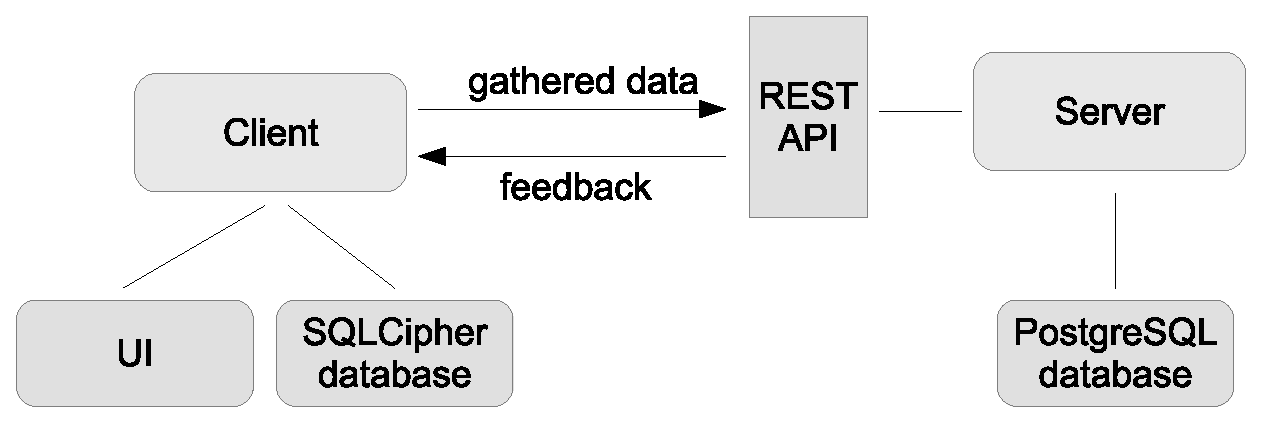
\includegraphics [width=0.9\textwidth]{images/Menthal_architecture}
  \caption{Menthal architecture}
  \label{fig:menthal_architecture}
\end{figure}

The client part consists of an Android application installed on a smartphone.
It keeps track of all the user activity during the day, such as unlocking the phone, number of calls and SMS, running applications, etc.
This data is structured as a key/value pairs, where the key is .. and the value is a particular event (e.g. ..).
The information gathering process is hidden from users, the application runs in the background, automatically sending data to the server once per day.
Menthal has a user interface to provide users with a feedback. 

\mnote{Menthal GUI}
The main screen shows a 'score' - the relative phone usage measurement.
Using this value, one could check how intensively he uses his phone today comparing to previous days statistics.
UI provides also additional functionality.
It shows overall daily/weekly/monthly statistics about the phone usage such as most used application, number of calls or the number of times user unlocked the phone.
After a short questionary it can display personality characteristics diagram, that includes five sides: extraversion, neuroticism, openness, conscientiousness, agreeableness.
Furthermore a user can check the list of contacts with whom he communicates more often over a period of time.
The next screen shows the daily time spenditure with the phone for the last 30 days.
The application is able to keep track of user mood, periodically checking his current state of mind.
Using smartphone's GPS receiver, Menthal can determine and show on map the user location.
Moreover the application gives an opportunity to put a time limit on a particular application, so when the limit is exceeded the phone warns a user about that.

\begin{figure}
\centering
\begin{minipage}{.5\textwidth}
  \centering
  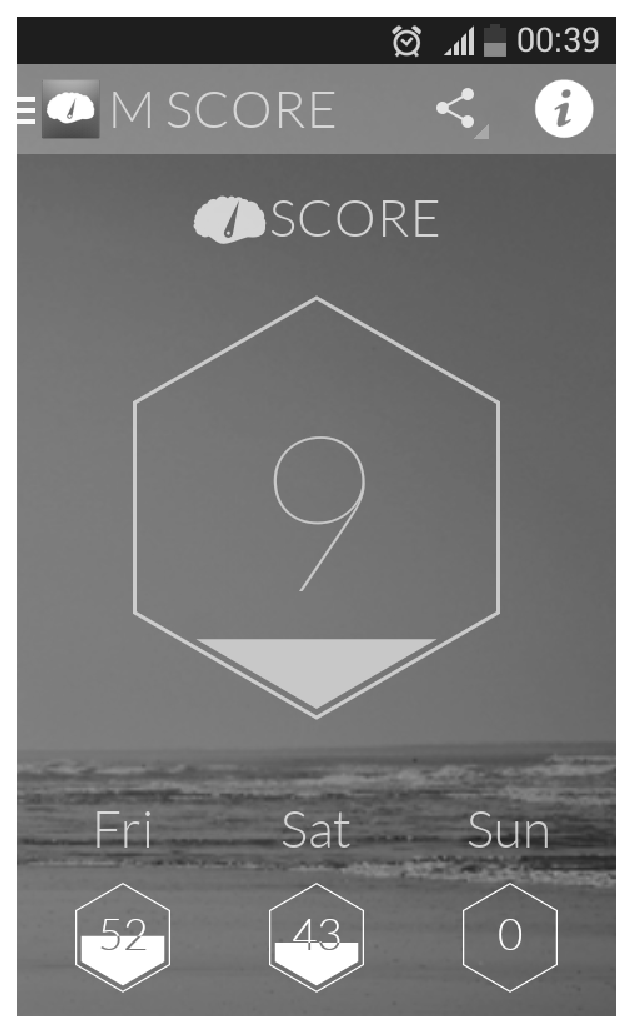
\includegraphics [width=.8\textwidth]{images/Menthal_GUI_mainscreen}
  \caption{Start screen}
  \label{fig:menthal_gui_mainscreen}
\end{minipage}%
\begin{minipage}{.5\textwidth}
  \centering
  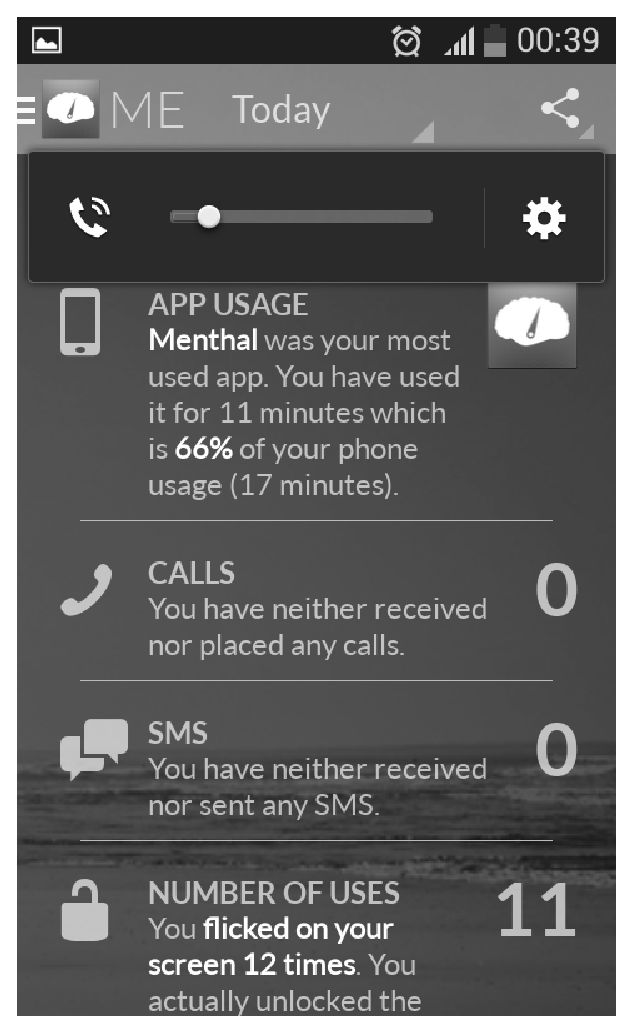
\includegraphics [width=.8\textwidth]{images/Menthal_GUI_me}
  \caption{Personal statistics}
  \label{fig:menthal_gui_me}
\end{minipage}
\end{figure}

\begin{figure}
\centering
\begin{minipage}{.5\textwidth}
  \centering
  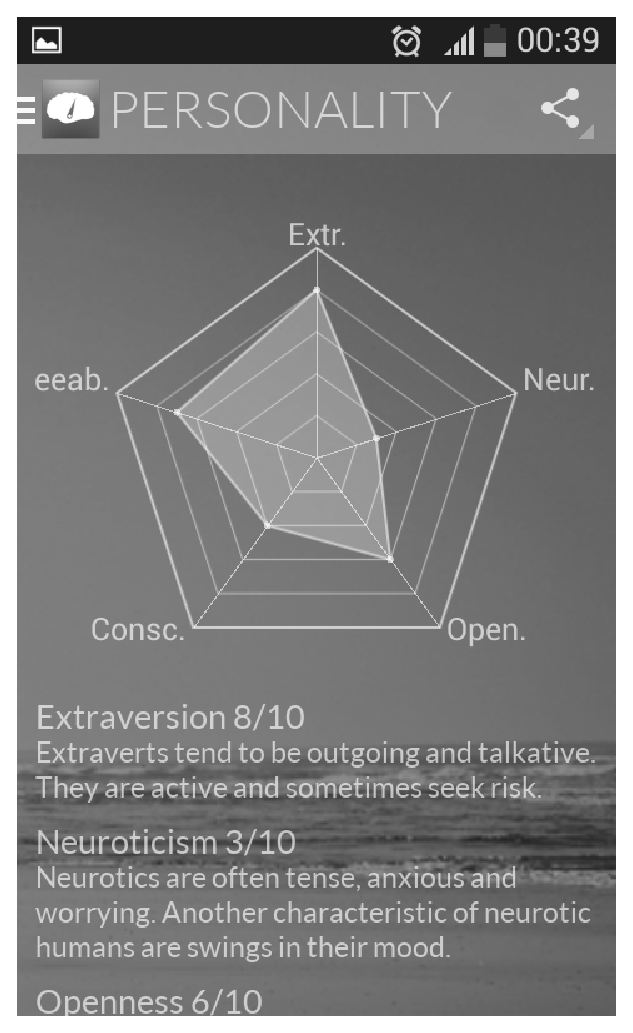
\includegraphics [width=.8\textwidth]{images/Menthal_GUI_personality}
  \caption{Personality characteristics}
  \label{fig:menthal_gui_personality}
\end{minipage}%
\begin{minipage}{.5\textwidth}
  \centering
  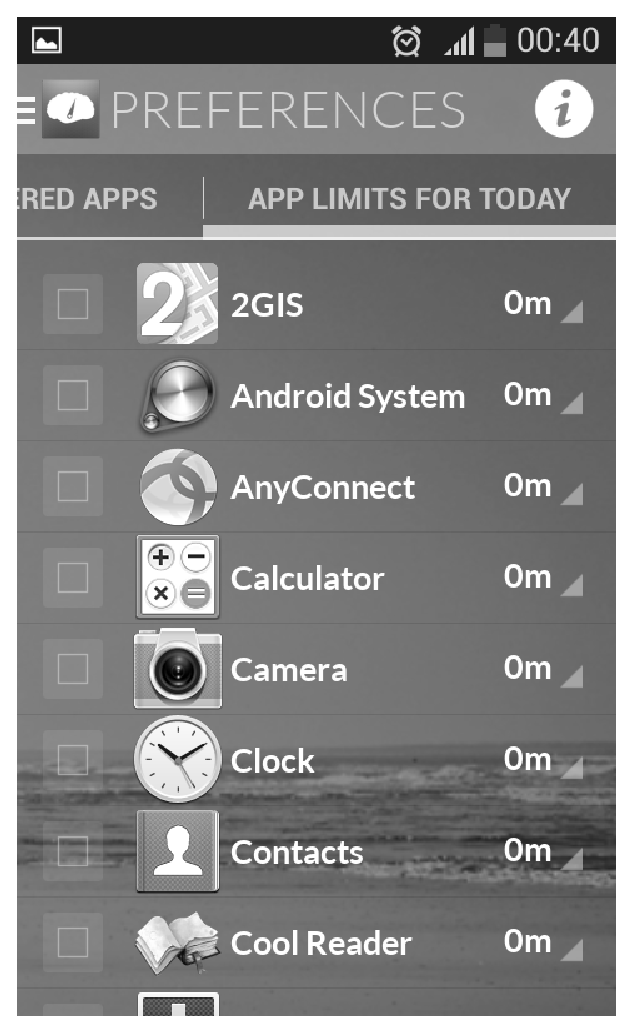
\includegraphics [width=.8\textwidth]{images/Menthal_GUI_preferences}
  \caption{Time limits preferences}
  \label{fig:menthal_gui_preferences}
\end{minipage}
\end{figure}

\mnote{information security}
Menthal uses secure connection, encryption of sensitive data and authentication mechanism to guarantee information security.
Communication between the client and the server goes through HTTPS.
This protocol is designed to provide a secure communication over a computer network. 
OAuth 1.0a protocol guarantees an authorization control.
On the phone the data is stored in SQLCipher database.
This database uses 256 bit AES encryption for storing information in a secure way.
Moreover, Menthal hashes the sensitive data, such as the contact names or the phone numbers via SHA2. 

% paragraph about sending patterns (Wifi, buffer) 
 
The problem of scaling becomes urgent when Menthal is covered in mass media.
The articles in newspapers and interview with a project leader lead to the explosive increase of the number of users.
Menthal obtains around 50 000 unique users, that has a significant influence on the application performance.
It becomes overflowed and is not able to write all incoming data into database, not to mention providing a feedback. 
% run out of id-s on one of the machines?
The architecture of the application is changed to meet the new requirements.

% ������ ���� ����� 
The most suitable architectural solution is taking an advantage of recently developed Lambda Architecture.
It is design specifically for handling large amounts of data.
The detailed description of Lambda Architecture is presented in Chapter 5 of this work.
Currently the process of moving Menthal to this architecture is conducted. 

Menthal recently gained popularity among users.
As it was mentioned almost 50 000 persons have this application installed on their phones.
All of these devices periodically send collected information to the server, that sums up to a vast amount of data.
Totally around 34Gb of information is received per day, that is almost 1Tb per month.
% number of machines
% stop with problem with Postgres

\chapter{Big Data Architecture}
\label{chap:big_data_architecture}

Traditionally, the process of making decisions is expensive and experiences significant error.
Simple reasoning is a straightforward approach, but it can work only till the certain point.
The main problem is that it can be easily ruined by the wrong assumptions.
Hence one would preferably use evidence based approaches that built on the accumulated data.
The most commonly used tools for this purpose are surveys and experiments, carried out on a control group.   
However, they both have significant disadvantages that makes the process of making decisions more complicated. 
On the one hand, surveys and experiments involve human resources, what leads to high expenses.
On the other hand, these approaches are also vulnerable to errors.
A lot of various reasons can cause an error, such as a survey composed in a wrong way, or a not representative control group.
 
Fortunately, this situation has changed dramatically in recent years.
First of all, data has become available for free, as a by-product of other processes (such as log files).
Moreover, constant reduction of data storage costs allows to warehouse enormous amounts of information, without troubling about the size limits.
Owing to the progress in the information technologies area, both transferring and processing of huge data volumes become easy.
All this gives us an alternative solution to the problem of making decisions that avoids the drawbacks of the strategies presented above.
The name of this solution is Big Data.

The main distinguishing feature of Big Data is that data collection is independent of use case.
Information is collected because it is available and cheap, with the hope that later on it can be used to answer a question that has not arisen yet.
For example, Facebook stores all available data about the users, like demographic information, geographic location, connections with other users, visited websites, clicked links, etc.
As a result it has a huge amount of data, which, with the right approach, can give lots of useful information. 
For instance, afterwards it can be used in targeted advertising, or for performing the social network analysis.

\authorsection{Big Data}{SP}
\mnote{Big Data}
There is no consensus about the origins of the term "Big Data", but most of the sources claim that it is first mentioned in the press in 2008.
People start actively using it since 2009 and it spreads quickly owing to its precise and capacious meaning. 
Big Data is characterized by its high (i) variety, (ii) velocity and (iii) volume. [reference]
All these three "v" constitute a criterion that allocates Big Data observation into a distinct sector of computer science, which requires ad hoc decisions and a special approach.

\mnote{Variety}
First, Big Data sources are highly diverse.
They differ in the type of produced data - it can be text, images, sounds, raw feed incoming directly from sensors, etc.
Each of these types, in turn, may have a different format.
For instance, text can be transmitted in various languages, coding, formatting and so forth.
Big Data sources also differ in the speed of data flow and the data purity.  
Some of the sources generate noisy information, while others can produce data, that does not need cleaning.
Moreover, Big Data differ in the way how it is collected, how urgently it should be processed and which storage capabilities are available for its warehousing.

\mnote{Velocity}
The diversity of Big Data sources causes the high velocity of data input flow.
For example, [Menthal]
Since data arrives at a high speed, there is a high chance that the velocity of its transmission and processing should also be high.
For instance, it can help to improve traffic in metropolitan areas, offering various travel alternatives for a vehicle, basing on analysis of incoming data about the situation on the roads.
Rapidity of data processing can be necessary in other cases as well.
Sometimes high processing speed can even be indispensable to life, when using in medicine, for example.
Special systems monitor the state of a patient, immediately alerting caregivers in the case of dangerous anomaly occurrence. 

\mnote{Volume}
In the end, massive sources variety, multiplied by high velocity of data generation, results in its enormous size.
For instance, by the end of 2013, the number of Facebook users reaches 1.23 billion.
Each of them not only has some profile information, but also communicates with other users, shares data, updates the timeline and so forth.
In total 2.5 billion content items are shared every day.
Let us assume that each of these events is stored as a JSON object and needs 2Kb on average.
That means that in the end of the year Google deals with 4.65Tb * 365 = 1.65Pb of information.
And it is only metadata, not including images and video files that require significantly more space. 
As a result, Facebook deals with storing and processing petabytes of data.

Another example is the information received from sensors.
Sensor is a converter that measures and transforms physical quantity into a digital signal.
Sensors find an application in various fields: manufacturing industry, transportation systems, meteorology, medicine, even modern smartphones have lots of sensors.
The key feature of a sensor is that often it does its job constantly, continuously producing the flow of information, what leads to the large volumes of data.
Nest Labs is an American company that manufactures sensor-driven thermostats and smoke detectors.
The population of United States is about 318 million, so if every hundredth resident uses at least one of Nest thermostats in the house, it sums up to 3.2 million devices.
One thermostat has a variety of sensors, like activity, temperature, humidity, illumination, etc.
They generate and transmit around 2Mb of data per day, or, consequently, 2.17Tb per year. 
The ability to process large amounts of information is the main benefit of Big Data analytics, since with its vast volume it is possible to construct better models.

\mnote{Batch Processing}
There are two fundamentally different ways of processing the Big Data, namely Batch and Real Time data processing.
In the first case, data is handled in batches, i.e. process collects the data until the batch size is obtained, and only after this the process can perform the necessary actions on a batch as a whole.
This gives several advantages.
Obviously, it becomes possible to process multiple operations in one request, instead of handling each operation individually.
That makes data treatment more efficient. 
To give a naive example how batching improves the performance, let us describe the problem of I/O operations.
I/O operations involve physical movement of mechanical devices (e.g. seek motion of hard drive).
Thus, the speed of sequential writes to a file is higher than random writes, because in the latter case additional time is spent for seek operations between each write.   
The same principle also works in general case, i.e. combining multiple operations in one batch can significantly enhance performance.
Batch processing can be done in the appropriate time, when the computing resources are less busy.
Furthermore, one can set a priority for each task, beginning with more urgent operations.
There is no need in a close supervision of a run, batch processing is mostly autonomous.
However, there is a significant drawback.
The results are always obtained with an arbitrary time delay.

\mnote{Real Time Processing}
Real time processing handles data at the moment of arrival. 
The advantage of the latter is that the results are ready almost immediately, which can be an essential requirement in such areas as medicine or security threat prediction. 
In spite of the fact that a certain delay is nevertheless exists, its duration is predetermine and is guaranteed to have a specified value.
That differentiates real time processing from batch processing.
This fixed delay length varies depending on the application.
In some cases 10 minutes to perform all the computations is still considered to be a real time processing.
However, in other cases, more than 1 second delay is unacceptable.
Real time processing makes the information always available and up-to-date.
These significant advantages results in rising popularity of real time processing, despite the fact that it requires greater effort to design and maintain.

\authorsection{Architectural Requirements}{SP}
There are some requirements that are common for most of the Big Data architectures.
Availability, reliability, scalability and performance are important attributes of a distributed architecture.
\mnote{Availability}
Availability means that a system operates properly at any given moment.
It can be calculated by the following formula: (total time - down time)/total time.
Consequently, availability depends on the sum of the time the system was down.
That means that even if the system fails every hour, but for negligible time, it is still considered to be highly available.

\mnote{Reliability}
On the contrary, reliability denotes the capability of a system to operate continuously without failing.
Reliability and availability are the opposite concepts.
The highly available system mentioned above is not reliable, because the intervals of working without failing are relatively short.
However, the system that is down for one hour but only once per month can be reffered to sufficiently reliable.  

\mnote{Scalability}
Scalability indicates the property to handle an increasing amount of work.
In informatics it means that the performance of the system can be enhanced using additional hardware resources.
There are two types of scaling, namely vertical and horizontal.
Vertical scaling means that the single node of a system is enriched, e.g. CPU is added to a computer. 
Horizontal scaling denotes the enlargement of a system by adding new nodes.
In the context of Big Data architecture the latter method is of great interest for us.
First, because of the decreasing computer price it becomes possible to build highly performant systems using commodity machines.
Second, in some cases the system should be distributed geographically.
For instance, adding new nodes closer to the customer can reduce the network load.

\mnote{Performance}
Performance is a quantitative characteristic of operation speed.  
This concept includes a variety of aspects, such as response time, processing speed, latency, bandwidth, etc.
With regard to extremely high volume and velocity of Big Data the question of system performance is a big issue.
For fair comparison of multiple systems performance a benchmark is used.
A benchmark is a sequence of tests that helps to estimate the performance of the system.

The world of Big Data introduces its own specific requirements for architecture design.
The file size can be enormous comparing to the standards.
It is not rare to work with a file of several gigabytes.
Storing the data in large files simplifies data processing.
The size of data itself is huge and it is more efficient to work with several large files than with great number of small files.

Another distinctive feature of Big Data architecture is that it is built on commodity machines.
A commodity computer is a moderately priced machine that is widely available for purchase.
The usage of inexpensive hardware helps considerably decrease the cost of the system.
It is especially relevant in the context of Big Data because of its overwhelming scales.
One of the well-known examples is the Google Lego server.
In 1996 two students, Larry Page and Sergey Brin, needed a cheap but capacious server to test the Pagerank algorithm on a huge data. 
They assembled it using 10 drives 4Gb each and a Lego enclosure. 
Nowadays Google uses commodity computers for building their computing clusters.

The direct consequence of the cheap hardware is the high failure rate.
Moreover, the large number of components also increases the probability of failure. 
Thus the system should be highly fault tolerant, with timely error detection and easy automatic recovery.

Big Data technology is an umbrella of various systems. 
Data has to be collected, processed, transmitted, stored, protected from attacks, etc.
The [Figure 3.1] shows the general flow of data within the Big Data concept.
Each of the presented steps involves a batch of technologies.
For example, depending on data type and size, one can choose SQL (MySQL, Oracle, Teradata, etc.) or NoSQL (Cassandra, MongoDB, Apache HBase, etc.) solutions for storing Big Data.
Similarly, depending on the application, Real Time processing (Storm, Spark Streaming, etc.) or Batch processing (Apache Hadoop, etc.) technologies are used. 
Thereby, it is apparent that no one general solution exists for every Big Data problem.

\begin{figure}
  \centering
  \includegraphics [width=0.9\textwidth]{images/big_data_flow}
  \caption{Big Data Flow}
  \label{Fig.3.1:Big Data Flow}
\end{figure}

Well thought-out structure of Big Data architecture is of big importance.
As it follows from the previous paragraph, Big Data architectures have to be targeted to each specific scenario.
For instance, architecture, designed for processing video data from a web camera, differs significantly from one for handling server log files.
Menthal, [Menthal: definition] mentioned above, deals with data, that consists of a bulk of key/value pairs. 
In the following sections we describe the existing Big Data architectures in the context of Menthal needs.

\mnote{Naive Approach}
It is natural to start with a naive approach, using widely available and easy to use technologies.
[Menthal: MySQL + what else?]
However, at a certain point, a naive approach cannot anymore sustain a constantly growing load.
Hence the biggest IT corporations conduct their own research in this area, designing specific architectural solutions for working with Big Data.

\mnote{Google Architecture}
Google is one of the well-known examples of such corporations.
Its activity directly relates to storing and processing of Big Data.
Google Search engine handles more than three billion searches every day.
Social networking service Google+ had 540 million users in 2013.
Gmail, Google's email service, had 425 million users in 2012.
These are just several examples of large-scale Google projects, that processes huge amounts of data.
Therefore, Google introduces a batch of solutions for building scalable systems. 

The overall structure of Google Big Data architecture is presented in [Figure 3.2].
The lowest layer is Linux kernel, that serves as a basis for Google File System.
Google File System is a scalable and highly available file system. 
These properties are achieved by replicating data across several machines.
Next, data can be efficiently processed by MapReduce framework.
This technology includes two steps - map, that performs filtering and sorting and reduce, that aggregates the output of map step to the final result.
Bigtable, a highly scalable database, provides a way to store massive amounts of information.
Finally, client application uses these technologies to perform highly scalable and distributed tasks.  
Let us explain in more detail the primary features and internal structure of these technologies.

\begin{figure}
  \centering
  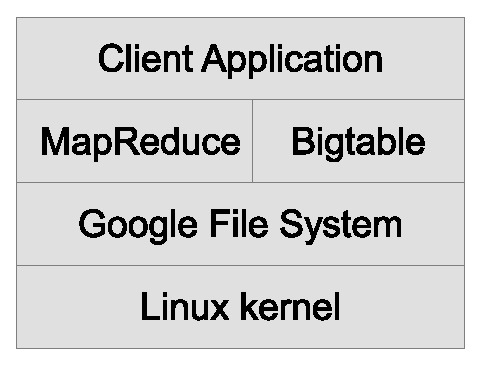
\includegraphics [width=0.9\textwidth]{images/Google_architecture}
  \caption{Big Data Flow}
  \label{Fig.3.1:Big Data Flow}
\end{figure}

\authorsection{Google File System}{SP}
[reference]
\mnote{Google File System}
Google File System (GFS) is a scalable distributed file system, which supports Big Data operations.
The underlying idea is the following: Google Search Engine and some other Google systems process vast amount of data, which is spread all over the world.
Hence the file system should be highly extensible, give an opportunity to use cheap hardware components and, consequently, be fault tolerate. 
Furthermore, it has some specific usage features.
Because of vast scales and cheap hardware, component failure is a commonplace.
The size of files exceeds several-fold the traditional standards, so a multi-gigabyte file is not unusual.
Most of the time the stored data stays unchanged and new data is only appended.
The append operation, in its turn, should provide the concurrent access for multiple clients.
GFS architecture design helps to meet all these requirements.

[Figure 3.3] illustrates the main components of the GFS Architecture.
Each GFS cluster contains one master server and several chunkservers.
The master has a "shadow" node, that provides read-only access when the primary master is down. 
Chunkserver stores chunks as Linux files on local disk.
Every chunk is replicated on several chunkservers for reliability.
One chunk combines multiple files and has a fixed size of 64 megabytes.

% Figure: according to [66]
\begin{figure}
  \centering
  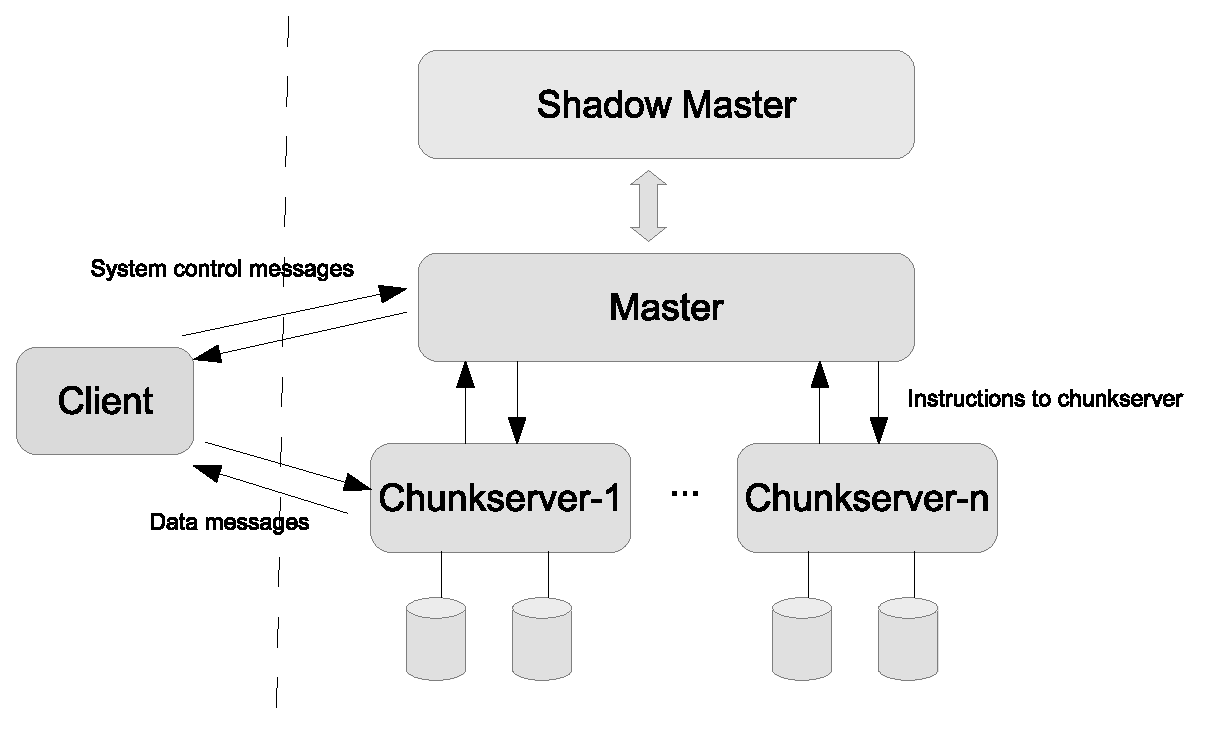
\includegraphics [width=0.9\textwidth]{images/GFS_architecture}
  \caption{Big Data Flow}
  \label{Fig.3.1:Big Data Flow}
\end{figure}

The large size of chunk gives several advantages.
Clients send requests to the master for chunk location less frequently.
A persistent TCP connection to the chunkserver for a longer time period allows to avoid network overhead.
The master node stores less metadata that provide a possibility to keep it in memory.

The master node manages the mapping from files to chunks, location of chunks, access control, garbage collection and some other tasks.
It does not persistently store the information about chunks location. 
On the contrary, it gives instructions to chunkservers and collects their states using periodic HeartBeat messages.
To prevent the master being a bottleneck, only file system control data goes through it.
For example, a client can ask the master node which chunkservers it should contact.
The master node returns the corresponding chunk handle and its replicas' location.
After receiving a reply, the client caches this information and can directly transfer data to the given chunkserver, dispensing master node from overload.
Clients and chunkservers do not cache file data.
Clients mostly work with files that are too large to be cached.
Chunkservers treat chunks as Linux files, therefore in this case caching is done by operating system.

\mnote{Operation Log}
To recover its state, the master uses the operation log.
The operation log consists of the chronometric information about critical metadata changes.
This log is replicated on several machines.
For the purpose of consistency, client receives a respond for operation only when corresponding log record is flushed to a local disk and the disks of all replicas.
To avoid the operation log being too large, the master makes a checkpoint each time when the log size exceeds a certain threshold.
In the case of failure, the master can load the latest checkpoint from local disk and replay it, recovering its state.
For storing checkpoint it uses a compact B-tree like data structure, that allows to map it directly into memory and perform fast lookups.
For performance reasons the new checkpoint is created in separate thread.
The ability of a server to restore its state does not depend on the way it was terminated.
Shutting down a server by killing the process is a normal procedure. 

\mnote{Mutation}
A mutation denotes a change of the contents or metadata of a chunk.
There are two types of mutations, namely writes and record appends.
In the former case data is written with a file offset specified by a client.
In the latter, GFS chooses an offset, and data (record) is appended with an append-at-least-once semantics.
Record append operation is atomic, i.e. it is treated as one continuous sequence of bytes. 
This allows multiple clients to append information concurrently.

\mnote{Lease}
Each mutation is replicated across several chunks.
To keep a mutation order consistent at all the replicas, GFS uses a technique of leases.
The master gives a lease to one of the replicas, that becomes a primary replica.
The primary chooses an order for all the chunk's mutations and each replica then follows this order when applying mutations.

The flow of write control is shown on [Figure 3.4] in more details.

\begin{figure}
  \centering
  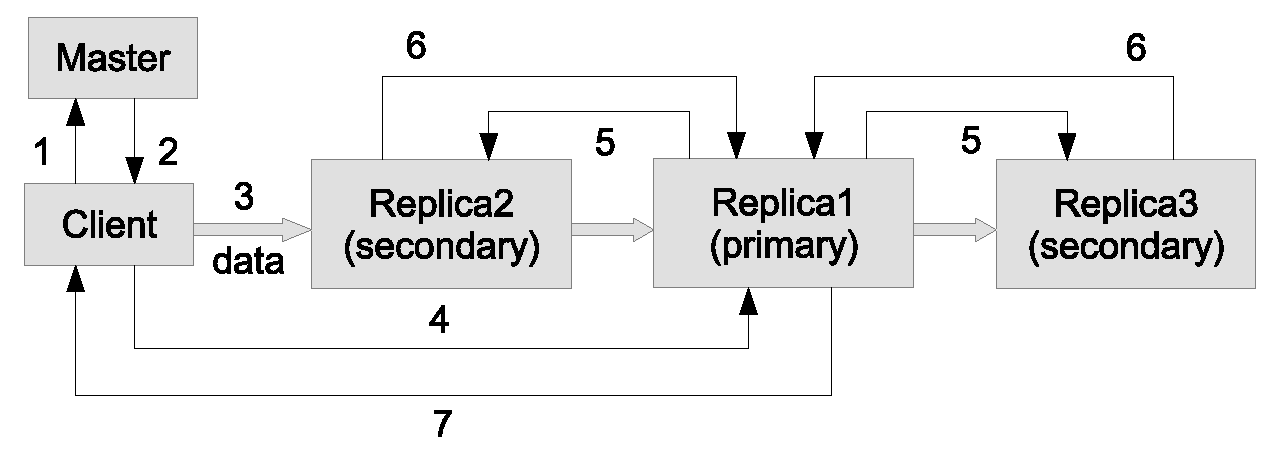
\includegraphics [width=0.9\textwidth]{images/write_control_flow}
  \caption{Big Data Flow}
  \label{Fig.3.1:Big Data Flow}
\end{figure}

1. The client sends a request to the master.

2. The master replies with a chunkserver, that holds the current lease, and the location of the other replicas.
If a primary replica (that has a lease) is not defined, the master chooses one. 
The client caches this information for the next mutations.

3. The client sends the data to all the replicas in arbitrary order.
Chunkservers store this data in an internal buffer cache. 

4. When the client receives acknowledgements from all the replicas, it sends a write request to the primary.
The primary picks serial numbers to all the mutations it has received and performs them in corresponding order.

5. All secondary replicas receive the write request forwarded by the primary.
Each replica applies mutations to its own state in the same order assigned by the primary.

6. The secondaries notify the primary about the completion of the operation.

7. The primary sends a reply to the client.
In the case of error occurrence at any of the replicas, the primary informs the client about them.
The write is considered to be successful, if the primary and an arbitrary number of secondary replicas succeeded.

GFS differs from traditional file systems in the way how it manages files and directories.
There is no possibility to list all the files in a directory in GFS, because it does not support per-directory structure.
It stores a mapping between full pathnames and metadata in a lookup table.
Prefix compression helps to efficiently represent this table in memory. 

The file deletion does not occur at once.
Firstly the master logs the event of deletion.
Than the system renames the file with a hidden name that includes the time of deletion.
The master performs a regular scan of the namespace and removes a hidden file, if it has existed for more than a specified time interval (e.g. 3 days). 

All the described features help the Google File System to successfully cope with a large-scale data processing workload.
GFS meets the storage needs of Google corporation.
Therefore Google uses GFS as the storage platform for many applications, both in research and production areas.
Another Google technologies, like MapReduce or BigTable are based on it.  	 

\authorsection{MapReduce}{SP}
[reference]
MapReduce model finds wide application in a variety of real world tasks.
For example, search engines use web crawling to gather a vast amount of information.
They process this information to create inverted indices, construct web graphs, figure out the most frequent search queries, etc.
Any of these tasks can be divided into two steps, namely Map and Reduce.
Map operation converts input data to a set of intermediate key/value pairs.
Reduce operation, in its turn, combines all the values that share the same key.
The advantage of the MapReduce abstraction is that it hides the implementation details from users.
This allows even not experienced programmers to easily construct parallel and distributed systems.

MapReduce shares the same requirements with other systems that work with large data sets.
It should provide high parallelization, be fault-tolerant and perform load balancing between nodes.
Applying Map and Reduce operations helps to parallelize large calculations.
Moreover, this makes simpler re-execution of a task that serves as a primary mechanism for fault tolerance.

Both Map and Reduce operations work with key/value pairs.
The user of MapReduce library determines the logic of these operations, specific to the given application.
The Map function receives an input key/value pair and produces a set of intermediate pairs.
The MapReduce library groups these intermediate pairs together by the key and passes the result to the Reduce function.
It passes them via iterator that allows to handle a large data set without keeping it in memory.
The Reduce function merges the values with the same key, possibly decreasing a given set of values.
One Reduce function invocation can give only a single output value, or even none.
[Figure 3.5] illustrates a pseudo-code for a simple MapReduce task.

\begin{figure}
  \centering
  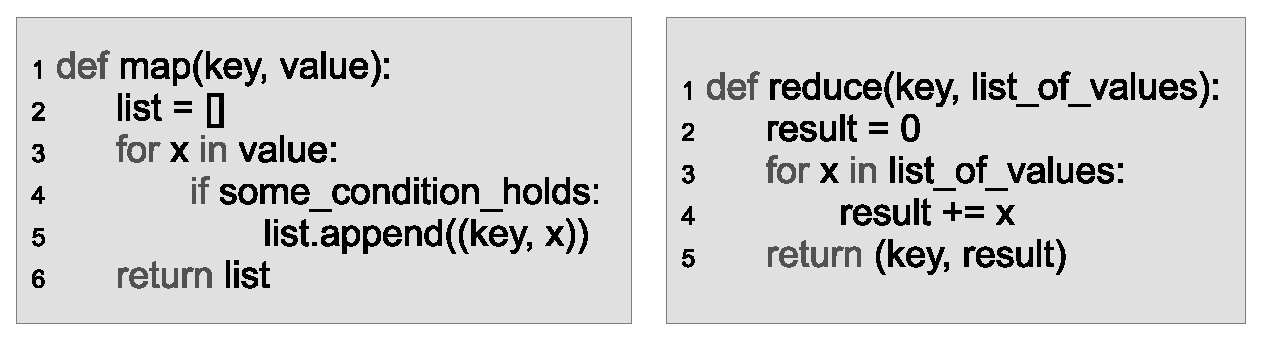
\includegraphics [width=0.9\textwidth]{images/MapReduce_pseudo_code}
  \caption{Big Data Flow}
  \label{Fig.3.1:Big Data Flow}
\end{figure}

We visualize the overall flow of a MapReduce operation in [Figure 3.6].
1. The MapReduce library divides the input files into M splits.
The size of one piece varies from 16Mb to 64Mb depending on the chosen settings.
User code invokes the MapReduce routine on several machines.

2. One of these machines is a master, while others are workers.
The master manages the workers, assigning to idle nodes one of M map tasks or one of R reduce tasks.

3. A worker that handles a map task reads the data from a respective input split.
It passes the parsed key/value pairs to the Map function.
The intermediate output of the Map function is stored in a buffer.

4. The MapReduce library periodically writes the buffered data into selected number of R local intermediate files.
Also it informs the master about the location of these files.

5. The master passes the locations to workers that handle a reduce operation.
A reduce worker reads the intermediate pairs from a specified location using remote procedure calls.
After compliting the reading, the worker groupes together all the pairs that share the same key.

6. These pairs are then passed to the Reduce function, one key and one or several related values at a time.
The output of the Reduce function is written to one of the output files.

7. After finishing all the map and reduce tasks, the MapReduce library returns the control to the user code.
The derived output files can be directly processed or be used as an input to another MapReduce task.

% BigTable

% - Facebook architecture
	
\chapter{Google Architecture}
\label{chap:google_architecture}

Google is one of the well-known examples of corporations that deal with Big Data.
Its activity directly relates to storing and processing of large volumes of data.
Google Search engine handles more than three billion searches every day.
Social networking service Google+ had 540 million users in 2013.
Gmail, Google's email service, had 425 million users in 2012.
These are just several examples of large-scale Google projects, that processes huge amounts of data.
Therefore, Google introduces a batch of solutions for building scalable systems. 

The overall structure of Google Big Data architecture is presented on the
Figure~\ref{fig:google_architecture}.
The lowest layer is Linux kernel, that serves as a basis for Google File System.
Google File System is a scalable and highly available file system. 
These properties are achieved by replicating data across several machines.
Next, data can be efficiently processed by MapReduce framework.
This technology includes two steps - map, that performs filtering and sorting and reduce, that aggregates the output of map step to the final result.
Bigtable, a highly scalable database, provides a way to store massive amounts of information.
Finally, client application uses these technologies to perform highly scalable and distributed tasks.  
Let us explain in more detail the primary features and internal structure of these technologies.

\begin{figure}
  \centering
  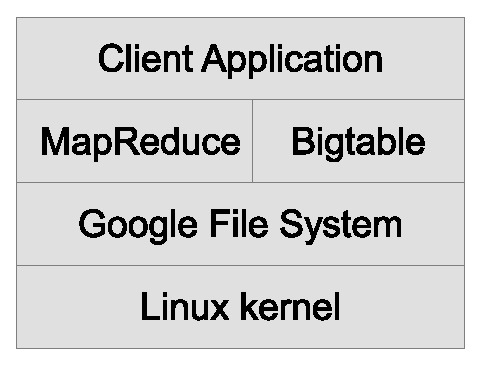
\includegraphics [width=0.9\textwidth]{images/Google_architecture}
  \caption{Google Architecture}
  \label{fig:google_architecture}
\end{figure}

\authorsection{Google File System}{SP}
[reference]
\mnote{Google File System}
Google File System (GFS) is a scalable distributed file system, which supports Big Data operations.
The underlying idea is the following: Google Search Engine and some other Google systems process vast amount of data, which is spread all over the world.
Hence the file system should be highly extensible, give an opportunity to use cheap hardware components and, consequently, be fault tolerate. 
Furthermore, it has some specific usage features.
Because of vast scales and cheap hardware, component failure is a commonplace.
The size of files exceeds several-fold the traditional standards, so a multi-gigabyte file is not unusual.
Most of the time the stored data stays unchanged and new data is only appended.
The append operation, in its turn, should provide the concurrent access for multiple clients.
GFS architecture design helps to meet all these requirements.

The Figure~\ref{fig:GFS_architecture} illustrates the main components of the GFS
Architecture.
Each GFS cluster contains one master server and several chunkservers.
The master has a "shadow" node, that provides read-only access when the primary master is down. 
Chunkserver stores chunks as Linux files on local disk.
Every chunk is replicated on several chunkservers for reliability.
One chunk combines multiple files and has a fixed size of 64 megabytes.

% Figure: according to [66]
\begin{figure}
  \centering
  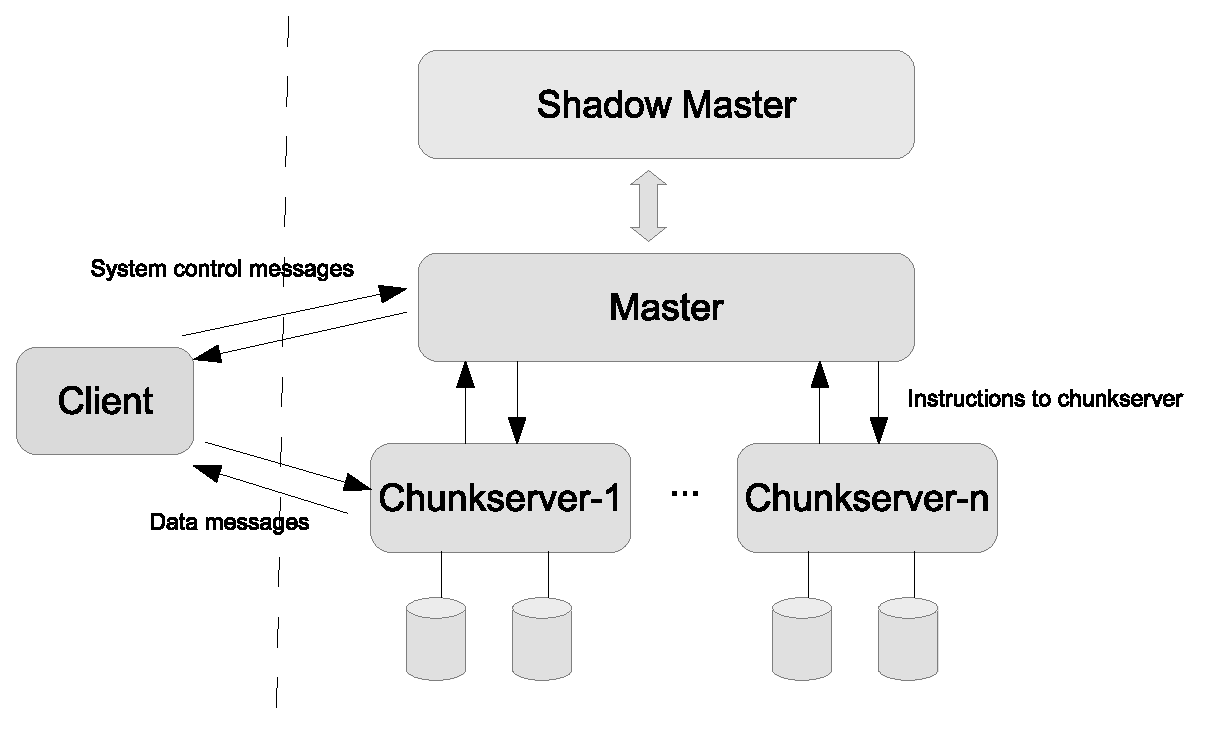
\includegraphics [width=0.9\textwidth]{images/GFS_architecture}
  \caption{GFS Architecture}
  \label{fig:GFS_architecture}
\end{figure}

The large size of chunk gives several advantages.
Clients send requests to the master for chunk location less frequently.
A persistent TCP connection to the chunkserver for a longer time period allows to avoid network overhead.
The master node stores less metadata that provide a possibility to keep it in memory.

The master node manages the mapping from files to chunks, location of chunks, access control, garbage collection and some other tasks.
It does not persistently store the information about chunks location. 
On the contrary, it gives instructions to chunkservers and collects their states using periodic HeartBeat messages.
To prevent the master being a bottleneck, only file system control data goes through it.
For example, a client can ask the master node which chunkservers it should contact.
The master node returns the corresponding chunk handle and its replicas' location.
After receiving a reply, the client caches this information and can directly transfer data to the given chunkserver, dispensing master node from overload.
Clients and chunkservers do not cache file data.
Clients mostly work with files that are too large to be cached.
Chunkservers treat chunks as Linux files, therefore in this case caching is done by operating system.

\mnote{Operation Log}
To recover its state, the master uses the operation log.
The operation log consists of the chronometric information about critical metadata changes.
This log is replicated on several machines.
For the purpose of consistency, client receives a respond for operation only when corresponding log record is flushed to a local disk and the disks of all replicas.
To avoid the operation log being too large, the master makes a checkpoint each time when the log size exceeds a certain threshold.
In the case of failure, the master can load the latest checkpoint from local disk and replay it, recovering its state.
For storing checkpoint it uses a compact B-tree like data structure, that allows to map it directly into memory and perform fast lookups.
For performance reasons the new checkpoint is created in separate thread.
The ability of a server to restore its state does not depend on the way it was terminated.
Shutting down a server by killing the process is a normal procedure. 

\mnote{Mutation}
A mutation denotes a change of the contents or metadata of a chunk.
There are two types of mutations, namely writes and record appends.
In the former case data is written with a file offset specified by a client.
In the latter, GFS chooses an offset, and data (record) is appended with an append-at-least-once semantics.
Record append operation is atomic, i.e. it is treated as one continuous sequence of bytes. 
This allows multiple clients to append information concurrently.

\mnote{Lease}
Each mutation is replicated across several chunks.
To keep a mutation order consistent at all the replicas, GFS uses a technique of leases.
The master gives a lease to one of the replicas, that becomes a primary replica.
The primary chooses an order for all the chunk's mutations and each replica then follows this order when applying mutations.

The flow of write control is shown on the Figure~\ref{fig:write_control_flow} in
more details.

\begin{figure}
  \centering
  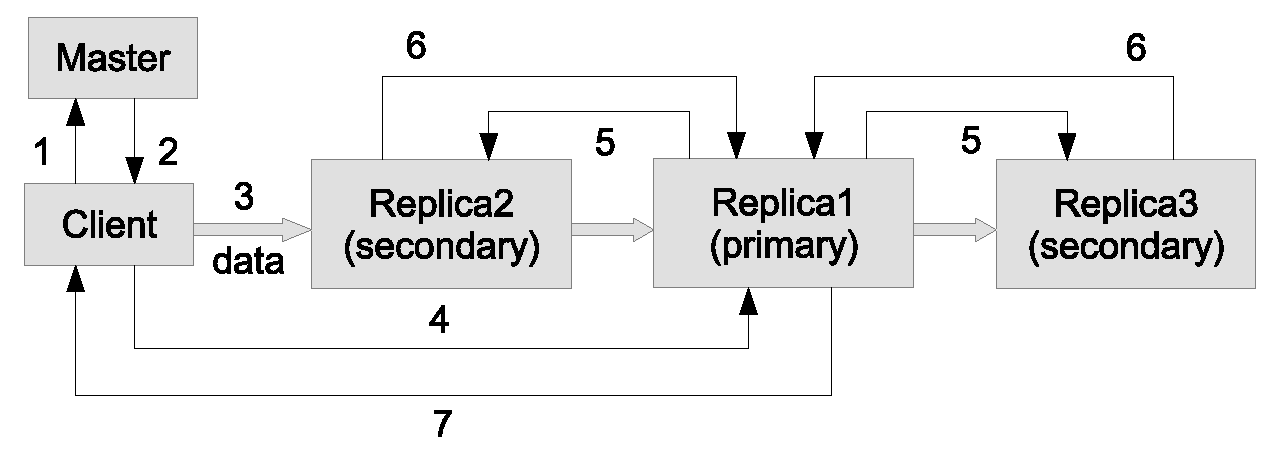
\includegraphics [width=0.9\textwidth]{images/write_control_flow}
  \caption{Write control flow}
  \label{fig:write_control_flow}
\end{figure}

1. The client sends a request to the master.

2. The master replies with a chunkserver, that holds the current lease, and the location of the other replicas.
If a primary replica (that has a lease) is not defined, the master chooses one. 
The client caches this information for the next mutations.

3. The client sends the data to all the replicas in arbitrary order.
Chunkservers store this data in an internal buffer cache. 

4. When the client receives acknowledgements from all the replicas, it sends a write request to the primary.
The primary picks serial numbers to all the mutations it has received and performs them in corresponding order.

5. All secondary replicas receive the write request forwarded by the primary.
Each replica applies mutations to its own state in the same order assigned by the primary.

6. The secondaries notify the primary about the completion of the operation.

7. The primary sends a reply to the client.
In the case of error occurrence at any of the replicas, the primary informs the client about them.
The write is considered to be successful, if the primary and an arbitrary number of secondary replicas succeeded.

GFS differs from traditional file systems in the way how it manages files and directories.
There is no possibility to list all the files in a directory in GFS, because it does not support per-directory structure.
It stores a mapping between full pathnames and metadata in a lookup table.
Prefix compression helps to efficiently represent this table in memory. 

The file deletion does not occur at once.
Firstly the master logs the event of deletion.
Than the system renames the file with a hidden name that includes the time of deletion.
The master performs a regular scan of the namespace and removes a hidden file, if it has existed for more than a specified time interval (e.g. 3 days). 

All the described features help the Google File System to successfully cope with a large-scale data processing workload.
GFS meets the storage needs of Google corporation.
Therefore Google uses GFS as the storage platform for many applications, both in research and production areas.
Another Google technologies, like MapReduce or BigTable are based on it.  	 

\authorsection{MapReduce}{SP}
[reference]
MapReduce model finds wide application in a variety of real world tasks.
For example, search engines use web crawling to gather a vast amount of information.
They process this information to create inverted indices, construct web graphs, figure out the most frequent search queries, etc.
Any of these tasks can be divided into two steps, namely Map and Reduce.
Map operation converts input data to a set of intermediate key/value pairs.
Reduce operation, in its turn, combines all the values that share the same key.
The advantage of the MapReduce abstraction is that it hides the implementation details from users.
This allows even not experienced programmers to easily construct parallel and distributed systems.

MapReduce shares the same requirements with other systems that work with large data sets.
It should provide high parallelization, be fault-tolerant and perform load balancing between nodes.
Applying Map and Reduce operations helps to parallelize large calculations.
Moreover, this makes simpler re-execution of a task that serves as a primary mechanism for fault tolerance.

Both Map and Reduce operations work with key/value pairs.
The user of MapReduce library determines the logic of these operations, specific to the given application.
The Map function receives an input a key/value pair and produces a set of intermediate pairs.
The MapReduce library groups these intermediate pairs together by the key and passes the result to the Reduce function.
It passes them via iterator that allows to handle a large data set without keeping it in memory.
The Reduce function merges the values with the same key, possibly decreasing a given set of values.
One Reduce function invocation most of the time produces a single output value, or even none.
A pseudo-code for a simple MapReduce task is illustrated below.

\begin{lstlisting}
def map(key, value):
	list = []
	for x in value:
		if some_condition_holds:
	 		list.append((key, x))
	return list

def reduce(key, list_of_values):
	result = 0
	for x in list_of_values:
		result += x
	return (key, result)
\end{lstlisting}

\begin{figure}
  \centering
  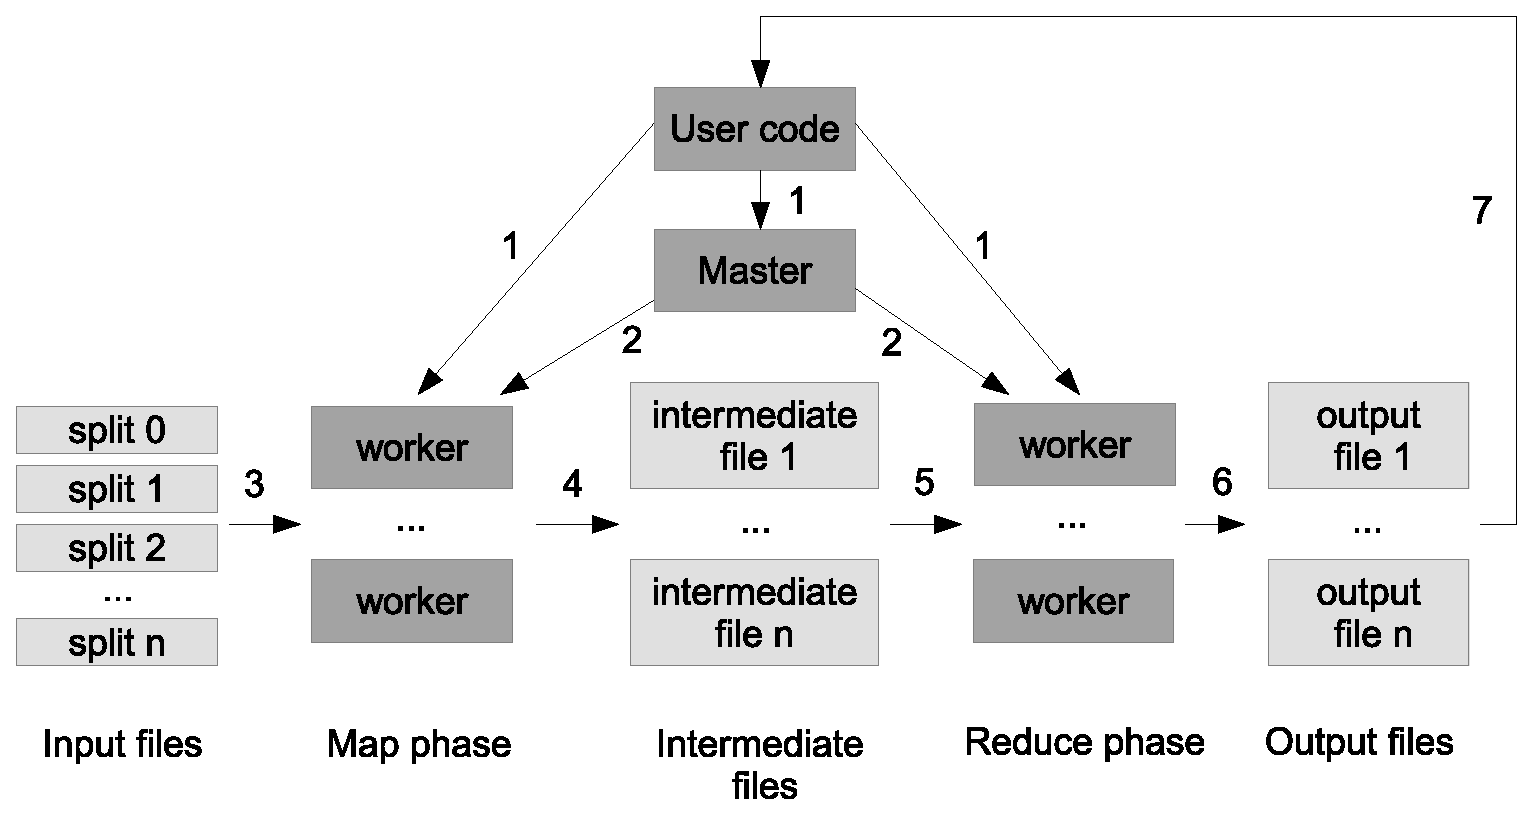
\includegraphics [width=0.9\textwidth]{images/MapReduce_operation_flow}
  \caption{MapReduce operation flow}
  \label{fig:mapreduce_operation_flow}
\end{figure}

We visualize the overall flow of a MapReduce operation in the Figure~\ref{fig:mapreduce_operation_flow}.

1. The MapReduce library divides the input files into M splits.
The size of one piece varies from 16Mb to 64Mb depending on the chosen settings.
User code invokes the MapReduce routine on several machines.

2. One of these machines is a master, while others are workers.
The master manages the workers, assigning to idle nodes one of M map tasks or one of R reduce tasks.

3. A worker that handles a map task reads the data from a respective input split.
It passes the parsed key/value pairs to the Map function.
The intermediate output of the Map function is stored in a buffer.

4. The MapReduce library periodically writes the buffered data into selected number of R local intermediate files.
Also it informs the master about the location of these files.

5. The master passes the locations to workers that handle a reduce operation.
A reduce worker reads the intermediate pairs from a specified location using remote procedure calls.
After compliting the reading, the worker groupes together all the pairs that share the same key.

6. These pairs are then passed to the Reduce function, one key and one or several related values at a time.
The output of the Reduce function is written to one of the output files.

7. After finishing all the map and reduce tasks, the MapReduce library returns the control to the user code.
The derived output files can be directly processed or be used as an input to another MapReduce task.

The MapReduce library has an optional Combine function that can be used for optimisation.
For example, let us consider the task of counting the number of words in English text.
Most probably it contains a lot of articles `a` and `the`.
Each Map task sends thousands of pairs <a, 1> to a single Reduce operation over the network. 
The Combine function can improve this situation by partial merging these pairs before sending them over the network.
Each machine that executes a Map function now also executes a Combine function.
Combine operation often uses the same code as Reduce one.
The difference is that the output of the former is stored in an intermediate file, while the latter writes it into the final output file.

The usage of Google File System (GFS) for storing input data helps to reduce the network bandwidth consumption.
GFS stores input data in blocks, copying each block on different machines (usually it makes 3 copies).
The master in MapReduce library knows which machine contains a replica and tries to assign a corresponding map task to this machine.   
When it is not possible, the master uses the nearest node to that machine.
This technology conserves network bandwidth significantly, especially when dealing with huge MapReduce operations.
 
The master keeps track of worker failures.
For this purpose it stores the state of each task and the identity of the worker that performs the task.
There are three types of states: idle, in-process and completed.
The behavior of the master in the case of failure depends on the type of the task (map or reduce) that failed.
When the map task fails, the master re-executes it on another worker.
Re-execution is required since the output of the map task is stored locally on the failed machine.
On the contrary, there is no need to re-execute the reduce task because global file system stores its output.
Sometimes a failure is caused by a defective record.
In this case the MapReduce library optionally can skip this record to continue the work. 
 
Stragglers is another problem that can obstruct the task completion.
Straggler is a machine that handles the last several map or reduce tasks too slow, keeping the whole system waiting for completion.
The MapReduce master uses a special mechanism to solve this problem.
On termination of an operation it executes the remaining in-process tasks on two different machines.
When either primary or backup worker completes computations, the task is considered to be completed.

Google Search engine widely uses MapReduce functionality for indexing, computing different statistics and analysing data.  
Moreover MapReduce can significantly facilitate the problems of data mining and machine learning.
Its key feature of dividing the computation into Map and Reduce phases helps to easily build distributed systems and makes the computation considerably more efficient.  

\authorsection{BigTable}{SP}
[reference]
Some Google projects deal with so large amounts of data, that common storage systems cannot sustain such a load.
For instance, personalized search, that stores user browser history and handles search queries based on the stored information about user activity.
It is necessary to warehouse each user's data.
Taking into account the huge number of Google Search users, the amount of data to be stored is also tremendous. 

The company introduces its own storage system for these purposes - a Bigtable.
It is a sparse, distributed, persistent multidimensional sorted map. [reference]
Bigtable uses three-dimensional mapping: row key, column key and timestamp are mapped to an array of bytes.
It is created to store petabytes of data in a distributed way.
As Google uses Bigtable in various projects, it puts different requirements on data size and latency of the storage system. 

\mnote{row keys}
The row key is represented by an arbitrary string with a maximum size of 64Kb.
Read and write operations under one row key are atomic.
Bigtable stores row keys in lexicographic order and dynamically partitions each row range.
One partition is called a tablet and serves as a distribution and load balancing unit.
For instance, when storing web pages with an URL as a row key, it is optimal to arrange pages from the same domain in one tablet.
In this case an URL like en.wikipedia.org/index.html is presented as org.wikipedia.en/index.html.

\mnote{column keys}
Bigtable groups column keys into column families, which serves as an access control units.
It means that each column family can have different access permissions (e.g. write access for one application and read only for another one).
It is common to store in one column family data of the same type.
One can store data under a column key only when a column family comprising this column key is created.
Number of distinct column families should be kept small, while each column family can contain unbounded number of columns.
The name of column key is presented as family:qualifier pair, where family should be printable and qualifier can be an arbitrary string.
For example, the column key name can look like language:en, where 'language' is a column family name and 'en' is a language ID. 

\mnote{timestamps}
Timestamps are used to store multiple versions of the same information.
A timestamp can be assigned in different ways.
On the one hand, Bigtable can use the time in microseconds as a timestamp.  
On the other hand, a client application can maintain its own unique timestamps.
Several versions of data are ordered such as the most recent version can be accessed first. 
Garbage collector processes the outdated data automatically using one of the two column family settings to detect the outdated versions.
The first setting allows to keep only the last \textit{n} versions of data, while the second setting allows to keep data that was written in the last \textit{m} days.

\mnote{Sawzall}
Bigtable uses a special language developed by Google to allow user to manipulate stored data.
The language is called Sawzall.
Scripts, written in this language, can execute on Bigtable server's address spaces.
Using Sawzall scripts one can filter, transform and make various summarization on data.

The major components of Bigtable are a master server, a number of tablet servers and a library linked into each client.
It is possible to dynamically add or remove tablet servers according to given workload.
The master assignes tablets to tablet servers, performs load-balancing, garbage collection.
Furthermore, it is responsible for creation of tables and column families.
Each tablet server controls a tablets set.
When a client sends a read or write request to the tablet, this request is processed by the tablet server.
Also the tablet server splits too large tablets.

The internal details of master-slaves interaction are similar to those mentioned above in GFS and MapReduce subchapters.
Analogously, the system does not transfer client data through the master and establishes a direct connection between clients and tablet servers.
It prevents the high load of a single master node.

A Bigtable cluster warehouses one or several tables.
A table contains a number of tablets. 
All the data that belongs to one row range is situated in one tablet.
Primarily one table contains only one tablet.
When the table becomes larger than a specified threshold, it automatically splits into several tablets.

\mnote{METADATA table}
The root tablet uses a special METADATA table to store the location of tablets.
The root tablet is a first tablet in this table.
However, it is never split in contrast to the rest of the tablets to keep the number of hierarchy levels constant.
Figure~\ref{fig:bigtable_tablets_hierarchy} illustrates the tablets hierarchy.
The METADATA table also stores logs of operations on each tablet.
This data can be used for preformance analysis and debugging.  

\begin{figure}
  \centering
  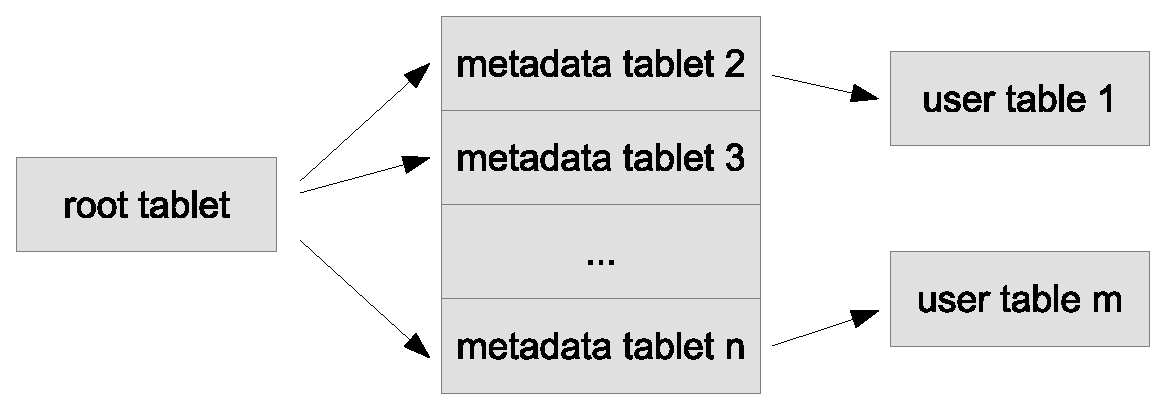
\includegraphics [width=0.9\textwidth]{images/bigtable_tablets_hierarchy}
  \caption{Bigtable tablets hierarchy}
  \label{fig:bigtable_tablets_hierarchy}
\end{figure}

\mnote{SSTable}
Bigtable stores data in special file format called SSTable.
Each SSTable consists of several blocks of a fixed size (64Kb by default). 
To locate blocks it stores their indexes, that are loaded into memory on opening the SSTable.
The blocks indexes considerably decrease the lookup time.
First the binary search is performed on in-memory index to find the needed block.
Than the appropriate block is read from disk.
The whole SSTable can be loaded into memory if necessary to perform lookup and scan operations avoiding touching disk.

A tablet can be recovered using a commit log.
This log contains all the tablet updates.
The most recent updates can be obtained from a memtable - a sorted buffer in memory.
The set of SSTables stores the older updates. 
A tablet server can read the METADATA table to detect the necessary SSTables for recovering.
Than the tablet server applies all the updates in order to restore the crashed tablet. 
  
A tablet server checks the incoming read and write operations.
The operation should be well-formed and the sender should be authorized to perform a mutation.
First the server writes a valid mutation to the commit log.
Then for write operation it inserts its content to memtable.
When the size of the memtable goes beyond the given threshold, the system frozes it.
It creates a new memtable and converts the frozen one into an SSTable. 
Read operation is performed on a merged view of the memtable and corresponding SSTables.

Periodically a merging compaction on SSTables and the memtable are used to create new SSTables out of old ones.
A regular compaction merges the memtable and a few SSTables, keeping the deletion information and deleted data.
A major compaction merges all SSTables into exactly one SSTable, cleaning deletion entries.
Bigtable performes the compaction mechanism regularly to keep the system up-to-date.

The variable number of tablets makes the system flexible and therefore easy to scale.
The implementation features provide good performance and high availability.
Bigtable is successfully used in many Google products, that proves the high quality of this storage system.
\chapter{Real time processing in the Big Data context [VI]}
\label{chap:real_time_processing}

\section{Something about Twitter}

\section{Bloom filter, other algorithms}

\section{Kafka paper}

\section{Speed Layer (for real time processing)}
\chapter{The Lambda Architecture [VI]}
\label{chap:lambda_architecture}

%New terms:
% view
% batch layer
% batch view
% serving layer
% speed layer
% real-time view
% raw data
% immutability

The Lambda architecture is a new solution for generic BigData systems \cite{MarzWarren201401}.
To answer queries it uses both batch and online processing.
It fulfills all requirements that such systems demand, e.g. scalability, extensibility, fault-tolerance, etc.
It provides human fault-tolerance, what is often overlooked in other approaches.
All its components automatically distribute computations across many machines.

%The core purpose of the Lambda architecture is to answer queries, having data, gathered during system's functioning.
%We consider any query as a function of the whole dataset, i.e. taking all available data, system can derive information, that answers specific query.
%The Lambda architecture is also able to answer queries that have not yet arised to the moment of the system's design or deployment.

The Lambda architecture uses both batch and online processing of data to answer queries fast as well as accurate.
It applies batch processing to all data to precompute specific data structures helping to answer queries with low-latency.
It also executes online incremental processing of arriving data, what helps to overcome delay of batch computations.

The Lambda architecture has all properties to be an effective and efficient BigData system.
It is robust and fault-tolerant.
It provides low-latency query answering.
It is scalable, generic and extensible.
It allows to make ad hoc queries, requires minimal maintenance, and is debuggable.

Important aspect of the Lambda architecture, that makes a difference with other approaches, is that human fault-tolerance is inherent.
Human fault-tolerance is a robustness of the system to mistakes in programming code.
This is important issue, because programmers always do mistakes.
As a result, deleting or updating the data in a wrong way is also possible.
The Lambda architecture overcomes this issue not allowing to delete or modify so far gathered data.

The Lambda architecture is a distributed system.
Every its part provides this property inherently.
That lets developer to concentrate on the logik and algorithms, instead of thinking about multithreading issues.

\authorsection{General structure}{VI}

System must provide information having gathered data from users and other sources.
Application of complex algorithms is often necessary.
Amount of data and rate of its arrival are heavy.
Those aspects makes system to preprocess indices and aggregations that provide useful information.
Batch processing is a good solution for that, nevertheless it has drawback - execution time is long.
Incrementall processing resolves this issue.
In combination these two approaches allow to design a system, that answers user queries with low latency as well as accurate.

The purpose of the system is to answer queries having data.
Let's consider an artificial example.
Suppose we have a website where people pose programming questions, and other answer them.
In this case the simplest query to the system is to return list of answers for a particular question post.
Another query is to find all posts containing given keyword.

One query is easy to answer, another requires application of complex algorithms.
It is pretty easy to get list of answers to the question post having its id.
You simply create hash-table that maps questions' ids to lists of answers' ids.
Search by keyword, or even phrase search, is much more complex.
To make it possibe we have to build specific inverted index, and this requires much more time to execute and to programm.
Let's further assume, that our system has to provide keyword search, using precomputed inverted index. 

Amount of data gathered with the time, as well as intense of arrival, can be huge.
Let's consider again our example website.
Assume that on average every second 5 questions and 20 answers appear.
Every post is about 100 words, each of about 8 unicode symbols.
The rate of incoming data is then $25*100*8*2=39$ KB per second.
It is about 3.2 GB per day.
This leads our system to be able to process such amount of data efficiently, as well as to rapidly reflect the state of inverted index with newly arrived posts.

Amount of data and complexity of algorithms demand to make computations, useful for fast answering queries, in advance.
The system precomputes specific data structures, that provide data, prepared as much as possible to directly answer specific queries.
We call these data structures \textit{views}\mnote{view}.
They store indices and aggregations of original data.
In our example we consider inverted index as a view.
In a query time it provides efficient search of all posts with particular keyword.

The basic approach is to precompute views in a batch mode.
The \textit{batch layer} \mnote{batch layer} of the Lambda architecture is responsible for that.
It takes the whole dataset, available so far, and executes batch computations on it.
Views that are the result of batch processing we call \textit{batch views} \mnote{batch view}. 
This operation is efficient, because all data is at once in disposal.
We can execute any algorithm, and produce any kind of index or aggregation.
It is also easy to programm, because there are such greate approaches as MapReduce.
This paradighm is inherently distributed and scalable.
In example with website we would use MapReduce to create inverted index having all posts.
It requires only several lines of code in the simplest case.

After batch layer has precomputed views, it places them into the \textit{serving layer}\mnote{serving layer}.
The serving layer is responsible for storage of batch views.
It also provides interface to get particular data records from them. 

Batch layer starts then computations again, considering now data, that has come during the last batch processing.
This loop goes on infinitely.
Batch processing always starts again from scratch using all available data.
When the batch layer stores computed views into the serving layer, it discards old ones.

Figure~\ref{fig:lambda_architecture} depicts general view of the Lambda architecture. 

\begin{figure}
  \centering
  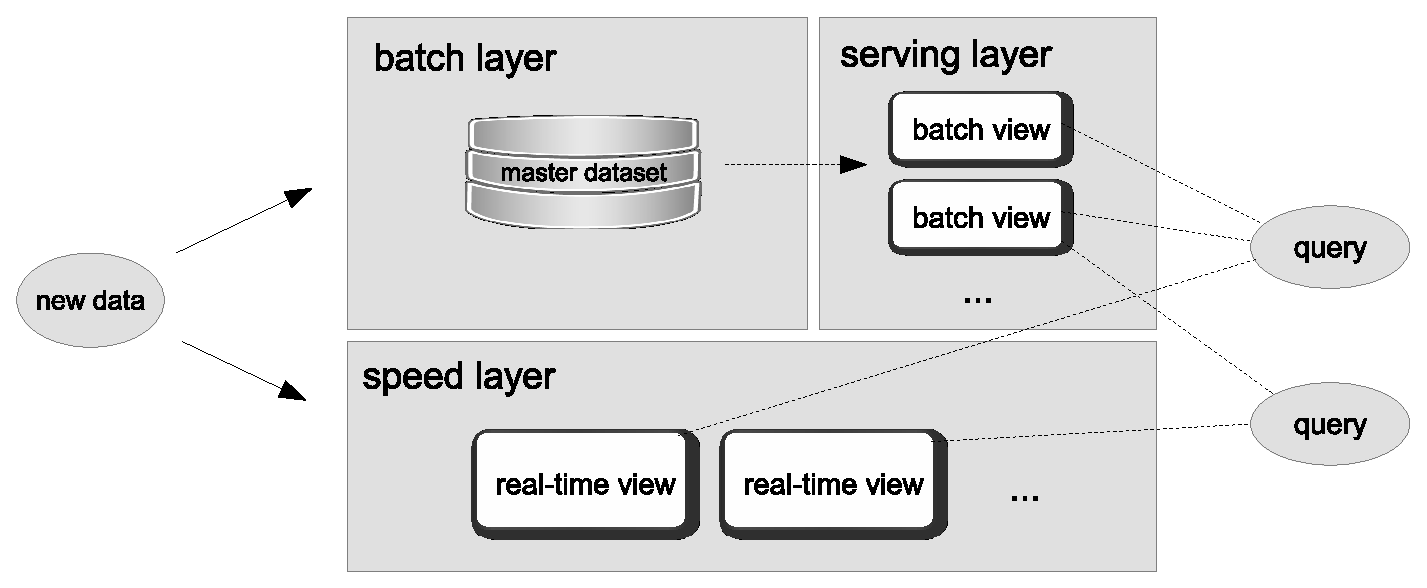
\includegraphics [width=1.0\textwidth]{images/LambdaArchitecture}
  \caption{General structure of the Lambda architecture. Batch and sevring layer are responsible for batch views, speed layer provides real-time views. To answer query system merges data from both types of views.}
  \label{fig:lambda_architecture}
\end{figure}

Batch computations, although easy and efficient, take long time to be done.
This cannot be underestimated, because on the BigData scale computations can last hours even if we setup cluster of thousends of machines.
In website example, assume our system has already been working for a year.
It has then about 800 millions of posts.
If we have a cluster of 100 machines, each has then to perform map-function 8 millions times.
If one execution of map-function takes 1 milisecond, it leads to 2.2 hours of total computations.
And we have not even counted reduce-phase.

As long as batch computations take much time, views are always outdated for several hours.
During this time new data arrives to the system, and it must be also counted in query answers.
This is not possible to solve using only batch processing.
Therefore, another approach is to apply.

To overcome delay of batch computations the Lambda architecture has additional component - the \textit{speed layer}\mnote{speed layer}.
It also computes views, but in incremental fashion.
We call them \textit{real-time views} \mnote{real-time view}.
As new data arrives, the speed layer updates incrementally real-time views.
Hence, they always has information from data, gathered during current batch processing.

Finally, to answer queries system uses both batch and real-time views.
Batch views contain result of the last batch processing.
Real-time views provide infromation from data, gathered after the beginning of the current batch processing.
Merging both types of views, system produces accurate and actual answers to the queries.
\section{Batch layer}

The batch layer is the heart of the Lambda architecture.
It is the place where all ever gathered data resides and being processed.
The batch layer executes two main tasks: storing of data arriving from outer sources, and processing of that data to create batch views, used for the low-latency query answering.
The first issue requires usage of a storage system, that provides fast appending, efficient batch reads, and no random reads/writes of data.
Computation of batch views demands application of distributed efficient batch processing algorithms as for example MapReduce.

\subsection{Data model}

%\mnote{Properties of data}
The batch layer requires usage of a specific data model to make the Lambda architecture scalable, highly efficient and fault-tolerant.
This data model is based upon four main notions.
\textit{Information} - the whole knowledge, that system holds.
\textit{Data} - collecting notion for records, strings, values, etc., kept in the system, so that they can not be derived from any other data.
\textit{Query} - a question that is asked to the system, and demands a piece of information that answers it.
\textit{View} - a data structure, that holds information directly useful for answering query.

\mnote{Raw data}
To answer as much different queries as possible, the batch layer stores only \textit{raw data}.
It is possible to derive from it data, particularly relevant for query, but not vice versa.
This is important, because the system does not know in advance all queries it will have to answer in the feature.
The more basic is the data, the more information can be possibly deduced from it.

In the current context, unstructured data is always better than normalized, because it is rawer.
As an example, let us consider the system, that stores users' search of a geographic location.
Suppose, that system stores all those queries for further analytics.
If it saves them normilized, or in other words parsed and mapped to a known geogrphic location, it can for certain queries save nothing or NULL value, because algorithm cannot execute correct mapping.
In other case, when the system stores raw string, that user typed, it can later on have this data properly parsed, if parsing and mapping algorithms are improved.
This example shows, that unstructured raw data is preferred to store in the batch layer.

\mnote{Data immutability}
The batch layer does not allow modification or deletion of data.
It only allows to append new records.
This propery is called \textit{immutability} of data.
It gives two crucial advantages.

Immutability drammatically simplifies complexity of the storage mechanisms.
This is because maintainance of modifications in the distributed environment is not an easy task.
To successfully update a record, the system must perform it for all replications, provide locks and prohibit simultaneous updates.
It has to maintain versions of the same record for different users.
Absence of all these and many other requirements saves from much of complexity.
The system is easier to understand, repair and improve.
It is much more safe from programming mistakes and consequent errors.

\mnote{Human fault-tolerance}
Another advantage of immutability is that mistakes in algorithms can not corrupt data anymore.
This property is called \textit{human fault-tolerance}, and it is very important, because programmers always do mistakes.
As a result, it is possible, that wrong code can incorrectly update or delete data.
When data is immutable, programmers' mistakes can only append wrong data to the dataset.
This can be later repaired by administrator, but all proper data is always safe.

Immutability leads to high growth of data volume, bevause everything last stored basically forever.
This is, however, not a problem, because, as we discuss later on in this chapter, the batch layer is purely distributed and scalable.
It allows to increase capacity of its data store to any extent, adding new machines at any time.

Immutability requires completely different data model, comparing to relational databases, that manipulate tuples of complex objects altogether.
In contrast, the batch layer stores each attribute of a logical tuple separately.
Each value has the timestamp of addition moment. 
Such technique allows to have the whole history of logical updates of all records.
The actual value is the one with the oldest timestamp.

\mnote{Eternal truthfulness of data}
Immutability gives one more important property of data, stored in the batch layer.
This is \textit{eternal truthfulness of data}.
When new record is added, no matter is it a new piece of data or update of an old data, it represents true information in that particular moment in time.
This never becomes false, because it describes event or state of the world, that is an occured fact.
This property implies, that the batch layer not only stores data, describing the state of the system, but also the history of its state changes.

\mnote{Master dataset}
Having defined the main properties of data, we can introduce the notion of the \textit{master dataset}.
The master dataset is the main storage, where all data, that ever arrived to the system, resides.
The batch layer is responsible for its maintainance.
If there is a fault of the master dataset - all data can be lost.
And data is of the most importance in this context.
Therefore, the master dataset must be carefully designed, set up and protected.
It must be saved from all types of failures, e.g software, hardware or human.
The master dataset is logically a large list of records.
When new piece of data arrives into the system, the batch layer appends it to the master dataset.
The more exact description of how the master dataset can look like will be discussed later on in this chapter.

%\mnote{Fact-based model}

%\mnote{Graph schemas and serialization frameworks}

\subsection{Data storage}

\mnote{Requirements}
\mnote{Usage of HDFS}

\subsection{Computation of batch views}

\mnote{Execution of functions}
\mnote{Application of MapReduce and Hadoop}

Answering particular query is often unreasonably expensive or even infeasible.
This is so, because amount of available data is huge, and because data is raw. 
Moreover, query answer demands usually a piece of information, that is far away from what raw data describes.
It requires often execution of complex algorthims on the whole dataset.
In the BigData context that can mean hours of processing, while low-latency response is typically a condition.

To solve this issue the batch layer precomputes batch views in advance.
Batch views contain derived data, that is a result of execution of specific algorithms and aggregations on the whole dataset.
They help in answering particular queries.
The batch layer creates batch views in advance, so that they are ready for low-latency response in the query time.

The batch layer computes batch views in the infinite loop.
After completion of data processing, it starts from the beginning.
Processing of all the data and creating batch views is a long operation.
It can take hours and even days to be done.
As a result batch views are always out-of-date.

Computation of batch views is inherently distributed operation.
Developer does not have to think about multithreading issues.
He only wrties simple one-threaded code, that is distributed then automatically in the cluster.
MapReduce is a perfect example of a batch processing.
\authorsection{Serving layer}{VI}

Serving layer is a place where the batch layer stores batch views.
When batch layer computes batch views, it loads them into the serving layer.
Then serving layer indexes them for a fast access.
Serving layer is represented by a specific distibuted database. 
It can be swaped by new data, but it does not have ability to make random
writes.
That simplifies things extremely, because opportunity to make random writes
brings most of complexity in databases.
One example of database that can be used for serving layer is ElephantDB.
\section{Speed layer}
\label{sec:speed_layer}

To overcome delay of the batch processing the Lambda architecture has the speed layer.
It applies the real-time incremental processing to arriving data.
The speed layer has higher complexity than the batch layer, because of the incremental nature of applied algorithms.
It provides usually approximated results, because algorithms, used for online processing, are often approximated.

The speed layer computes real-time views, that are similar to batch views in the sense, that they store data useful for fast answering queries.
Real-time views contain data, observed during ongoing batch processing in the batch layer.
The speed layer also prepares indexes on those views, that allow to answer queries ``on the fly''.

\subsection{Computation of real-time views}

To compute real-time views, one could consider the same approach as for batch views, but use only new data for computations.
This would simulate batch processing on the much smaller scale.
Nevertheless, if we want to achieve latency of miliseconds, such approach is not going to work.
Batch processing even on the scale of several gigabytes is not possible to do in miliseconds.

To solve this issue there is a completely different approach.
Real-time views are not considered as a function of a recent data, that has arrived during current batch processing.
Instead, they are the result of the function of a new data, that just came, and of their previous state.
Basically, it is an incremental update with a small piece of data, everytime it arrives.
This normally leads to only approximated answers to the queries, provided by real-time views.
But this is again not a problem, because error does not accumulate for too long.

\subsection{Data storage}

Speed layer must obey low-latency requirement, and must allow application complex incemental algorithms.
Having such demands, storing of real-time views requires several properties to be fulfiled: ability to make random reads and writes, scalability and fault-tolerance.
Ability to make random reads is particularly important to make answering queries fast.
Ability to make random writes is necessary, because of the need to apply incremental algorithms, that always demand this property.
Real-time views must be scalable, because amount of data to process can still be of a huge size.
That means, that distribtuion to many machines must be supported.
Fault-tolerance is as usual must be provided via replications of data in the real-time views.

There are many storage systems, that fulfil these properties.
They are usually called \textit{NoSQL databases}\mnote{NoSQL database}.
They store data using different data models than relational databases.
We have already briefly discussed one of such system, namely ElephantDB, that was useful for storing batch views in the serving layer.
One can choose specific database, that fulfils his or her requirements to data representation.
Sometimes batch and real-time views has the same data format.
But it is not always the case, because it is not always easy to execute the same function in the batch and in the incremental way.
Also, as long as real-time views have to be updated incrementally, they have more complex data structure.
Because of those factors, it often happens, that real-time views represent data differently, than batch views.

\subsection{Issues of incremental computations}

We have already discussed the difference between incremental and recomputation algorithms.
Batch computations imply, that computations of a specific function is executed on the whole dataset.
This is usually easy to program, even though can take much time.
In case of incremental computations, building of real-time view is going continuously.
It is usually more efficient, but can lead to accumulation of error, especially if programming mistake takes place.

The important aspect to discuss it a relation of incremental computations and a so called CAP theorem.
The CAP theorem states, that consistency and availability are not possible simultanously to achieve, when data is partitioned.
The meaning of the CAP theorem is that it is possible to make the system completely available, but it can sometimes return not yet actual data, or it is possible to make it truly consistent, but it can sometimes provide now response for a request, because data is not yet propogated to partitions.

There several ways of how to design the system, so that it provides consistency or availability completely, or has a tradeoff between them.
System is fully consistent, if it updates all replicas of a piece of data at once, and only then allow to access this data.
It is fully available, if it stores an update as a new temporal record, and then tries to merge it with the real data in the system.
This can take time, and reading of that data can return old values.

To achieve a tradeoff there so called \textit{conflict-free replicated datatypes} (CRDTs).
They provide eventual consistency working in a distributed fashion.
For example the G-Counter allows to maintain a counter, that allows only incrementation.
It stores different versions of an integer counters in different replicas, and the merge them to provide correct results.
There is unfortunately no way to aboid this complexity, and to make the system fully consistent and available at once.

\subsection{Expiration period of real-time views}

Real-time views, though more complex than batch views, but have only transient nature.
They are discarded every time, when batch layer completes processing of batch views.
Batch views then contain all information, that real-time views gathered during the last batch processing. 
Such temporal nature of real-time views saves from accumulation of error, and leads to eventual accuracy of query answering.

The simplest solution of discarding old real-time views is to set expiration time or period.
But it suffers from unstability of the duration of batch processing, that can vary every time.
Because of that, more robust, generic solution were proposed.

Let us consider a new information system, that does not have yet any data.
On the first run of batch processing the master dataset is empty.
But it still takes time, let say 10 minutes, because of overhead for creation of empty views, indexes, and so forth.
The speed layer gathers during this first batch processing data, and to its end has already real-time views, containing data, processed during this 10 minutes.

When the second start of batch computations runs, it consider the first 10 minutes of data, that resides now in the master dataset, for processing.
The speed layer continues to update real-time views.
Let's say the second batch processing takes 15 minutes.
To its end batch views have the reflection of the first 10 minutes.
Real-time views reflect all 25 minutes of system's life.
Now the part of them, that was built during th first 10 minutes can be discarded.

When the third batch processing starts, it considers data gathered during 25 minutes.
The online processing in the speed layer has updates now views, that has 15 minutes of processed data, gathered during the second batch processing.
Let's say the batch processing takes 18 minutes now.
When it finishes, batch views reflect the first 25 minutes of data, whereas real-time views reflect 33 minutes of data, starting after 10 minutes of the system's functioning.
Now real-time views must leave only reflection of the last 18 minutes of arriving data.

To make it possible, two sets of real-time views must be maintained.
The speed layer then switch between them after each finish of the batch processing.
Each set of real-time views store them results of processing during two consecutive batch runs.
This can look redundant and expensive, but is actually not, because real-time views store only small data, gathered during short time.

\section{Requirements compliance}

Robust
Fault-tolerant
Responses with low-latency
Scalable
Generic
Extensible
Allows ad hoc queries
Requires minimal maintenance
Debuggable
\section{Distributivity}

I'm not sure about this section
\chapter{Components}
\label{chap:components}
% we have described many technologies in previous cgapters
% for our architecture we have chosen the following technologies
% they will be discussed in greater details

% storage/persistent streeming/real time processing scala(or additional technologies/surrounding)

\section{Storage systems}

\subsection{HDFS [VI]}
\label{subs:HDFS}

The Hadoop Distributed File System (HDFS) is a distributed data storage that provides high throughput data access, fault-tolerance, ability to hold big datasets consisting of large files \cite{HDFSArchitecture1, HDFSArchitecture2}.
The Apache Software Foundation has developed HDFS originally for its web search engine - the Apache Nutch.
Today it is a widely-used distributed file system, that is an infrastructure for such distributed computational frameworks as Hadoop, Storm, etc.
HDFS allows to use cheap commodity hardware, because it does not require much computational or storage power for one particular node.
It is written in Java, hence, any platform with JVM \cite{JVM} can run HDFS's software.
HDFS supports standard hierarchical file organization with directories and files.

%\subsubsection{Use cases and requirements}

HDFS provides high throughput data access, because it is designed for usage in the BigData world.
Applications, that use HDFS, require fast writing and reading of files of gigabytes and terabytes in size.
HDFS is suitable for the batch processing, and it is important to say, that low-latency is not a goal property.
It allows to operate with the large number of files.

Fault-tolerance, detecting of failed machines, and recovering from inconsistent state of the file system are inherent properties of HDFS.
This is a key property, because disk failures and machine failures in general, happen more often, than we could think.
When we consider a cluster of hundreds and even thousands of nodes, this is actually a normal case.
Google has made a deep research on this topic, and has found out that 8\% of hard drives fail in two years \cite{Pinheiro2007}.
This statistic shows that it is reasonably expected that in the large cluster there are always machines that are out of service.

HDFS has a simple file storage model.
It holds every file in a coherent way, so that it can be only written, and not changed any more.
Only one client writes the file to the file system, but many clients can then read it.
This model has a name \textit{write-once-read-many}, and it helps to provide high throughput data access.

HDFS lets an opportunity to move computations into the cluster, instead of moving data from the cluster to where computations are executing.
This is proven to be much more efficient, because moving data creates high network congestion.
When the data is of a very high volume it is important aspect to consider.

HDFS is written in Java, what allows to run it on practically all platforms and any hardware.
The only requirement for a machine to use it in the HDFS-cluster is that it has running JVM.

%\subsubsection{General structure}

HDFS consists of two main elements: NameNode and DataNode.
These are applications that run on JVM.
They both do not require any particular operational system or hardware, and use local file system for storage of HDFS data pieces.

NameNode is a master program of the cluster.
It stores meta information about the file system's namespace, regulates access of the clients to files, maintains consistent state of the file system, initializes operations like create, rename or delete file.
NameNode is of the highest importance, because its failure can be dangerous for the whole system.
It runs usually on a special separated machine.
The fact that there is only one master node greatly simplifies system's structure, its maintenance and analysis of errors.
Data never flows through the NameNode.

DataNode is a program that holds data.
Each machine in the cluster runs usually one DataNode.
DataNode executes read and write requests directly from the clients.
It also performs creation, deletion and replication of blocks, when NameNode gives such instructions.

DataNodes hold files in blocks.
Standard size of a block is 64 Mb.
Normally, each block resides on the different DataNode to provide high reading throughput.
Every file has replication factor, that defines the number of its replicas.
If replication factor is for example 3, than each block of this file has 3 copies on different machines.
This provides fault-tolerance in case of disk or other hardware failures.

Applications access HDFS using Client program, that provides interface to do write and read requests.
When Client writes, it asks NameNode to give a list of DataNodes to write replicas of the first block.
Then it accesses DataNode directly and makes write of the block.
DataNode in its turn sends write request of this block to another DataNode, that is in the list for replications.
And so on, until the block has all its replicas written.
When block is written, Client asks about new list of replicas for the next block.
When Client reads, it asks NameNode for the list of replicas of the first block, sorts it by the distance in the network topology, and then gets it from the nearest replica.
Then the same for the next block and so on.
You can see the overall structure of HDFS and the way of its functioning on the Figure~\ref{fig:HDFS}.

\begin{figure}[h]
  \centering
  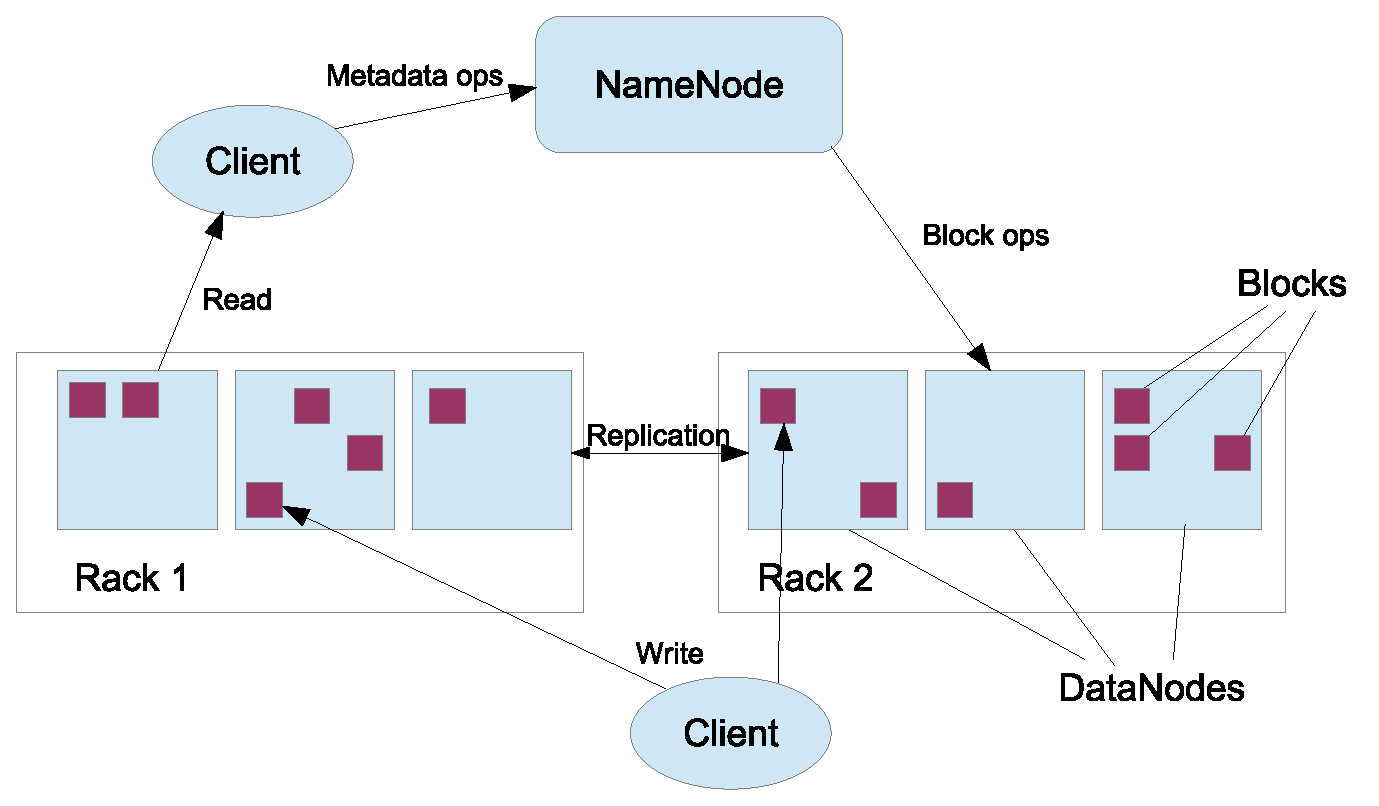
\includegraphics [width=0.8\textwidth]{images/HDFS}
  \caption{Overall structure of HDFS.}
  \label{fig:HDFS}
\end{figure}

%\subsubsection{Replications}

HDFS stores large files reliably, so that failures of particular machines can lead to an unrecoverable loss of a part of a file with a very small probability.
It also provides high throughput, placing blocks of files onto different DataNodes, to give parallel access of many clients to many files in the cluster.
The number of replicas and the block size are configurable parameters for every file.
Replication factor also can be changed for already existing files.

Cluster consists of the number of racks.
Rack is a group of nodes, that reside usually near to each other physically.
This helps to avoid redundant network usage, and to make replication algorithms more efficient.

The current replicas placement policy for the most common replication factor of 3 is as follows.
Put the first replica onto the DataNode in the rack, local for accessing client.
Put the second replica in the same rack, but onto the other DataNode.
Put the third replica onto the DataNode in another rack.
This approach gives both high fault-tolerance and near to optimal access rate.

%\subsubsection{Robustness}

One of the main goals of HDFS is to provide fault-tolerance from hardware failures.
For this sake, each DataNode sends periodically a Heartbeat signal to the NameNode, to notify about its state.
If the DataNode's machine fails, the NameNode does not receive Heartbeat signal, and marks this DataNode as out of service.
The NameNode starts then re-replication of blocks, that resided on the failed machine.
Another condition to make re-replication is increase by the client of the replication factor of a particular file.

When the piece of data arrives to the client, it can be corrupted during transfer in the network or because of a IO failures.
To provide integrity of data, HDFS has a checksum mechanism.
When a block of file is written, its checksum is also written to the file system.
Then, when client reads a block, it also receives checksum and able to match block.

HDFS manages balance in the cluster.
If there are DataNodes that has free space below set threshold, file system moves part of data from that nodes to others, that have more free space.
This is done automatically, and does not allow to accumulate data in the part of the file system, decreasing its access throughput.

There is a staging mechanism in HDFS, that helps to avoid network congestion.
Client, that writes data to the file system, does it in portions.
It accumulates the whole block in the local cash file, and only then makes flush to the DataNode.

\subsection{Redis [VI]}

Redis is an open source key-value in-memory data storage \cite{Seguin2012} \cite{Redis}.
It affords blazingly fast and simple tool for maintaining data inside of a single application or a cluster.
Redis is very easy to deploy, learn and use.
It provides 5 data structures, e.g. string, list, set, ordered set and hash, that are useful for different tasks, and give a powerful tool in combination.

\subsubsection{Basics}

Redis is a key-value store, that allows to hold all data of your application.
Redis lets to create many databases and switch between them.
For one database it maintains one global map of keys to values.
Although Redis is in-memory database system, it swaps data continuously to disk to provide persistance in case of application's failure.
This is also important in a distributed environment to have global data available between applications.

Record in Redis is a key-value pair.
The key is always a string.
It does not contain data, that your application manipulates, but it identifies piece of data, that you want to store.
The value can be of different types, but in any case it is a meaningful peace of data, that you store in the database.

Redis provides many useful and at the same time simple commands to work with data.
The two simplest commands are $SET$ and $GET$, that let to store a key-value pair into database, and to get value by key, respectively.
This is an example of how you can use these commands:
\begin{verbatim}
> SET server:name "SERVER1"
OK
> GET server:name
"SERVER1"
\end{verbatim}
There many commands to work with data structures, that Redis provides.

Redis allows to query only values by keys.
You cannot find a key, this is a crucial difference with classical relational databases.
And if you do not know a key, you can not find a value.
There is a command $keys$, that returns all keys, stored in the database, but it is strongly advised not to use it in production application, because it does a linear scan through all the keys, what can be very slow.
Another point is that operation of receiving a value by a key works in constant time, basically instantly.
This makes Redis blayingly fast and useful, because grow of the database does not affect its performance.

Redis stores the database to disk every minute if at least 1000 keys has been changed.
It makes less swaps, if you change less number of keys.
It does swap completely as a snapshot.
There is an alternative way to set Redis to make appending swaps.

\subsubsection{Data structures}

The basic data structure in Redis is a \textit{String}.
Keys are always strings.
Values can be of any type, but String is the most popular, because it represents atomic piece of data.
As a String you can store not just something simple like name of a user or his password, but also complex objects like JSON object, for example:
\begin{verbatim}
> SET users:user001 '{"firstname": "john", "lastname": "smith"}'
\end{verbatim}
Redis provides standard commands to work with strings, e.g. $STRLEN$, $GETRANGE$, $APPEND$, etc.
If you store numeric value as a string, you can work with it as with integer.
Redis has several useful commands for this case, e.g. $INCR$, $INCRBY$, $DECR$, $DECRBY$, $SETBIT$, $GETBIT$.

The first complex data structure is a \textit{List}.
List is simply an array of values identified by a key.
There are specific commands to work with lists, e.g. $LPUSH$, $RPUSH$, $LRANGE$, $LLEN$, $LPOP$, $RPOP$, etc.
The values of the list can by anything, not only strings.
This gives powerful tool to store complex combined data.

Set

Sorted set

Hash

\subsubsection{Features}

Transactions

Expiration

Publication and Subscriptions

Monitor and Slow Log

Sorting

Scanning

Scripts

\subsubsection{Administration}



\section{Real time processing systems}

\subsection{Storm [SP]}

Batch processing is not applicable for real time computing.
Hadoop, the best known tool for batch processing, is helpless when it is needed to handle streaming data and obtain immediate result.
The main advantage of real time processing, the guaranteed time delay between a request and a result can be broken simply because the waiting time for the next batch is too long.
Therefore new systems, designed for real-time processing, have appeared.
One of such systems is an open source project named \textit{Storm}.

Storm is a \textit{complex event-processing} (CEP) system.
Complex event processing means gathering data from different sources, combining it and making conclusions from it.
For example, such system keeps track of significant changes in traffic reports or stock market feeds and immediately responds to them. 

Storm is implemented in a dialect of the Lisp language named Clojure.
Clojure is a functional language like Lisp, but it also supports multithreaded programming.
Clojure runs on the Java Virtual Machine, however applications within Storm can be written in Java, Scala, JRuby, Perl and PHP.
Moreover, one can use a Structured Query Language adapter for streaming data directly into Storm topoloy.

\mnote{Storm architecture}
The Storm cluster has a master node called \textit{Nimbus} and \textit{worker} nodes.
Nimbus assignes tasks for workers and monitors failures.
There is a deamon called \textit{Supervisor} on every worker node.
The supervisor is responsible for starting and stopping worker processes assigned by Nimbus.
ZooKeeper coordinates the interaction between Nimbus and Supervisors.
It stores the state of all the nodes, making the system stable to failures.
If any of the nodes is killed, ZooKeeper immediately restarts it, enhancing Storm cluster stability.
ZooKeeper is described in more details later in this chapter.

The basic concept of Storm is a \textit{topology}.
It is a graph of computation, that shows how data should be processed and passed between the nodes.
One can implement a topology in any programming language, because topology definition is a Thrift structure.
Thrift is a framework that allows to develop cross-language services.	

The data stream consists of an unbounded set of \textit{tuples}.
A tuple can contain both standard data types (integer, float, byte array) as well as user-defined types.
Every stream has its own ID.
The sources of streams called \textit{spouts}. 

The next important Storm primitive is \textit{bolt}.
Figure~\ref{fig:storm_architecture} shows the interaction between spouts and bolts.
The stream of tuples originates from a spout and goes through a sequence of bolts.
Every bolt performs a transformation on incoming data stream, like aggregating, filtering, or interaction with external parts such as databases.
A bolt can receive information from several spouts and stream it to multiple bolts.

\begin{figure}
  \centering
  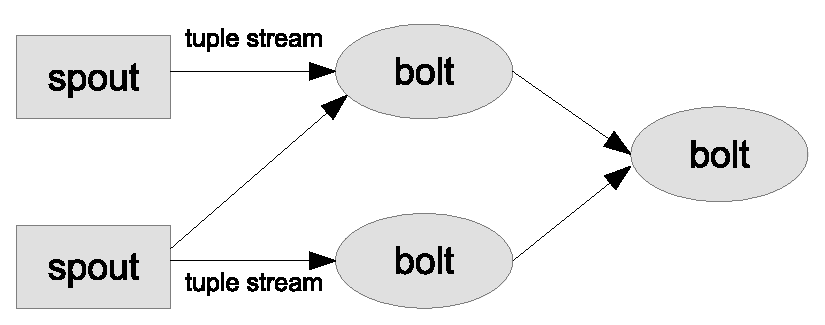
\includegraphics [width=0.5\textwidth]{images/storm_architecture}
  \caption{Storm architecture}
  \label{fig:storm_architecture}
\end{figure}

For example, MapReduce word counting example can be easily implemented with Storm.
Such system counts how many times each word occures in a given input data.
In the case of Storm one needs 
(1) a spout to generate text data, 
(2) one bolt to implement the Map function for word tokenisation and 
(3) one bolt to implement the Reduce function for aggregation the amounts of words occurences. 

Storm allows to group the stream of tuples in different ways.
For instance, shuffle grouping randomly distributes tuples to bolts such as each bolt receives approximately the same number of tuples.
Field grouping partitions tuples according to contained fields.
Also other grouping methods exist, including the custom grouping.

The Listing~\ref{lis:simple_storm_topology} represents a simple topology.

\begin{lstlisting}[caption=Simple Storm topology, label=lis:simple_storm_topology]
java TopologyBuilder builder = new TopologyBuilder();
builder.setSpout("myspout", new TestSpout(), 10);
builder.setBolt("mybolt1", new TestBolt(), 3) .shuffleGrouping("myspout");
builder.setBolt("mybolt2", new TestBolt(), 2) .shuffleGrouping("mybolt1");
\end{lstlisting}

Here topology consists of one spout and two bolts.
The stream of tuples originates from \textit{myspout}, then it is passed to \textit{mybolt1} and finally to \textit{mybolt2}.
In both cases tuples are grupped using the schuffle grouping method.
The integer numbers in \textit{setSpout} and \textit{setBolt} define the amount of parallelism for the node.

The implementation charasteristics of Storm lead to high performance and guaranteed fault tolerance.
It uses ZeroMQ for passing messages between the tasks.
Messages are automatically serialized and deserialized to Storm primitive types.
The usage of this message queue helps to avoid intermediate queueing, thus improving performance.
Furthermore, Storm guarantees the processing of every tuple.
In the case of a fault during message processing, a tuple is replayed from the spout.
There is also a fault detection mechanism on task level, when the failed task is quickly reassigned to restart the processing.
Storm has supervisors to manage the processes, that leads to efficient usage of resources.

Storm cooperates with message queue systems in such a way that every message is fully processed.
It builds a tuple tree, that reflects the motion af all the tuples.
Only when every message in the tuple tree is processed, a tuple is considered to be fully processed.

To give an example, let us take a message queue that supplies a spout with messages.
When the spout takes a message from the queue, the message state changes to 'pending'.
In this state it cannot be sent to other consumers.
Moreover, all the messages in pending state are returned to message queue if their consumer disconnects.
Storm assignes a unique id to the message, if it is not given by the message queue.
Using this id Storm can keep track of this message during processing.
The system receives this message when the \textit{nextTuple} method of the spout is called.
The spout emits the message along with its id to the consuming bolts.
When a tuple is fully processed, the \textit{ack} method of the original spout is called. 
In the case of time-out Storm calls the \textit{fail} method of the same spout.
Only when \textit{ack} or \textit{fail} method is called, the spout sends an ack or fail message to the message queue.
The message queue cancels the pending state of the message, taking it off the queue in the case of success and putting it back otherwise.

Storm can process not only the tuple trees, but also directed acyclic graphs.
It happens when an output tuple is anchored to several input tuples.
\textit{To anchor} means to specify a link in the tuple tree.
Multi-anchored tuples often appear during streaming aggregation or joining.
 
As it was mentioned, Storm tracks every tuple using its unique id.
Additionally, as each tuple exists within a tree, it knows all the tuples ids of this tree.
For example, if a bolt emits a new tuple, this tuple carries the ids of spout tuples received by this bolt along with its own id.
Such storage mechanism is used	because when the tuple is acked or failed, it should inform Storm about its dependencies to restore the state of the tuple tree.  

The acker task is responsible for acking the tuple.
First, Strom stores the mapping between an acker task and a spout tuple id.
As every tuple keeps ids of spout tuples in the tree it exists within, it knows the acker tasks it should communicate with.
A tuple informs an acker task when the tree is fully processed and the tuple is acked.
Second, the acker task should send a complition message to the spout task that emitted this tuple.
For this purpose, on creation of a new tuple a spout task notifies the appropriate acker task that its task id is linked to that spout tuple.

For acker task tracking the huge tuple trees explicitly is not efficient.
Thus Storm uses a special tracking strategy.
An acker task stores a map: on the one side it has a spout tuple id and on the other side a pair of values.
One of the values is a task id the spout tuple originates from, and the other is an 'ack val', the 64 bit number.
The 'ack val' represents the state of the tuple tree without storing it in memory.
This number is a result of XOR operation on all created and acked tuple ids of the tree.
Therefore, when the 'ack val' is equal to zero, it means that the tree is completed.

\subsection{Spark [VI]}

Spark is a framework for distributed data processing \cite{Zaharia2010} \cite{Zaharia2013} \cite{Spark1} \cite{Spark2}.
It provides a tool to work with large datasets and streams of data, and to make complex queries on this data.
Spark has several abstractions for representation of data and streams.
The first one - Resilient Distributed Dataset (RDD) - is an object, distributed in the cluster, that contains data to process.
Another one is a Shared Variable - variable, that can be used among the cluster as a counter or lookup table.
One more abstraction is a Discretized Stream (DStream) - representation of a data stream also in a distributed fashion.

\subsubsection{Data model and batch processing}

To initialize Spark you first create a SparkContext object, that is responsible for a connection of your program to Spark.
It allows to specify properties of your application, and also options of how Spark should run, for example in local mode or on the cluster.
SparkContext gives an access to different parameters and properties of execution environment.

\textit{Resilient Distributed Datasets}\mnote{Resilient Distributed Datasets} (RDDs) is a main abstraction in Spark, that represents dataset in a distributed fashion.
RDD is essentially a readonly collection of elements.
It is fault-tolerant, so that if one partiotion is lost, the whole collection can be recovered.
RDD does not need to exist physically on the cluster nodes.
Instead, it is a lazy object, that can lay in a robust data storage, and be computed on the fly, when computations require particular pieces of data.

There are two methods how to obtain an RDD object: parallelizing exisiting collection in the driver program, and using external dataset.
Existing collection is any collection of data, e.g. array, list, set, etc., that you in fact have in the program.
When you create an RDD object in this way, elements of a collection are copied to a distributed dataset, that you can use than in parallel.
You can specify the number of slices, that is the number of tasks, each machine in the cluster will then execute for this collection.
External dataset is an external file.
It can reside in the local file system, and in the distributed file system like HDFS.
The simple example of what you can do with the external text file, is to count the sum of lines' lengths using functions $map$ and $reduce$ of an RDD object. 
Additionally, you can obtain RDD by transforming another RDD, or by changing persistance of an existing RDD, but this methods are derived in some sense.

RDD supports two types of operations: \textit{transformations} \mnote{transformation} and \textit{actions}\mnote{action}.
Trnsformation creates a new RDD object from existing one.
An example is a $map$ function, that processes each element of an RDD object using specified function, and returns a new RDD object as a result.
Action executes computations on an RDD object, and returns a value.
$Reduce$ is an example of action.
It aggregates all elements giving in the RDD object and return the resulting value.

Transformation in Spark is a lazy operation, in the sense that it is computed only when action operation requires its result to produce output.
This makes execution more efficient when there is a chain of transformations before final action, because your application does not receive then intermediate RDD objects, but only final resulting value, that is usually much smaller.
Nevertheless, there are cases, when you want to compute different actions on the same transformation.
Then it is meaningful to have RDD object of this transformation computed once, and to have a handle to it in your program.
For this case there is a method $persist$, that allows to materialize RDD object.
This is also possible to persist RDD object on disk.

Next we present a simple program, that counts the sum length of all lines in a text file:
\begin{verbatim}
JavaRDD<String> lines = sc.textFile("data.txt");
JavaRDD<Integer> lineLengths = lines.map(s -> s.length());
int totalLength = lineLengths.reduce((a, b) -> a + b);
\end{verbatim}
Example is taken from \cite{Spark1}.
Here we create an RDD object from external file, set $map$ function to count length of the line, and set $reduce$ function to sum up lengths of lines.
Execution starts only when $reduce$ function is called, because, as we discussed, transformations are lazy in Spark.

Normally, when you pass arguments to any function, that executes on the nodes of the cluster, they are simply copied and there is no feedback to the driver program.
Sometimes it is useful to have global variable or lookup table, that all nodes can access.
Spark supports the notion of \textit{shared variable}\mnote{shared variable}.
There are two types of shared variables: \textit{broadcast variables} \mnote{broadcast variable} and \textit{accumulators}\mnote{accumulator}.
Broadcast variable represents readonly value or dataset, that is useful for all nodes as a lookup table or global predefined value.
It is copied to every node using method $broadcast$ of $SparkContext$.
There are efficient algorithms in Spark to make this transfer fast.
Accumulator is distributed counter, that allows all nodes to add up to the global numeric variable.
It can be created using method $accumulator$ of $SparkContext$.
No node can read this value or do anything else than incrementation, what makes its implementation easy and fast.
Only driver program is able to read accumulator's value.

\subsubsection{Streaming processing}

Streaming in Spark is an extension of a Spark engine, described in the previous section.
It can process data stream in a distributed manner.
Spark Streaming receives data from the input stream, divides it into blocks, each represented as an RDD, and passes this sequence of blocks to the Spark engine.
It can work with different sources, e.g. message queue server (Kafka), web service (Twitter API), or regular TCP socket.
Processed data can be there stored to the filesystem or database.
The main abstraction for streaming processing in Spark is a Discretized Stream or DStream.
It is internally a sequence of RDDs.
Several DStreams can be combined into one chain for application more complex algorithms. 

Similarly to Spark engine, you must create $SparkStreamingContext$ object to work with Spark Streaming.
It allows to adjust environment for processing, set properties like local or cluster mode, number of threads used, and many others.
One important propery is the batch interval.
It defines the time of gathering data from the input stream, before creating DStream and sending it to the Spark engine.

\textit{Discretized Stream} \mnote{Discretized Stream (DStream)} or DStream is the main abstraction in Spark Streaming.
DStream can be the input stream, as well as intermediate stream, generated after processing of input stream of data.
It is essentially a chain of RDD objects, and provides a stream of data, that is to process by Spark.
Each RDD represents batch of data in the period of time, that is specified in the $SparkStreamingContext$.
Figure~\ref{fig:SimpleDStream} depicts simple DStream.

\begin{figure}[H]
  \centering
  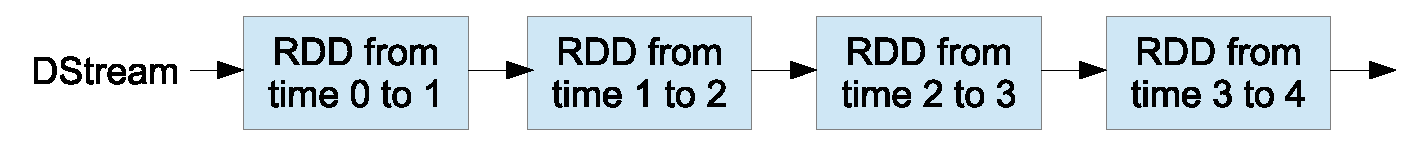
\includegraphics [width=1.0\textwidth]{images/SimpleDStream}
  \caption{Representation of a simple DStream.}
  \label{fig:SimpleDStream}
\end{figure}

Every operation you want to apply to DStream is applyed to every RDD object in the stream.
This implies, that transformation on the DStream produces new DStream.
All these transformation are executed by Spark Engine in a standard batch fashion.
Figure~\ref{fig:DStreamWithTransformation} depicts how it works.

\begin{figure}[H]
  \centering
  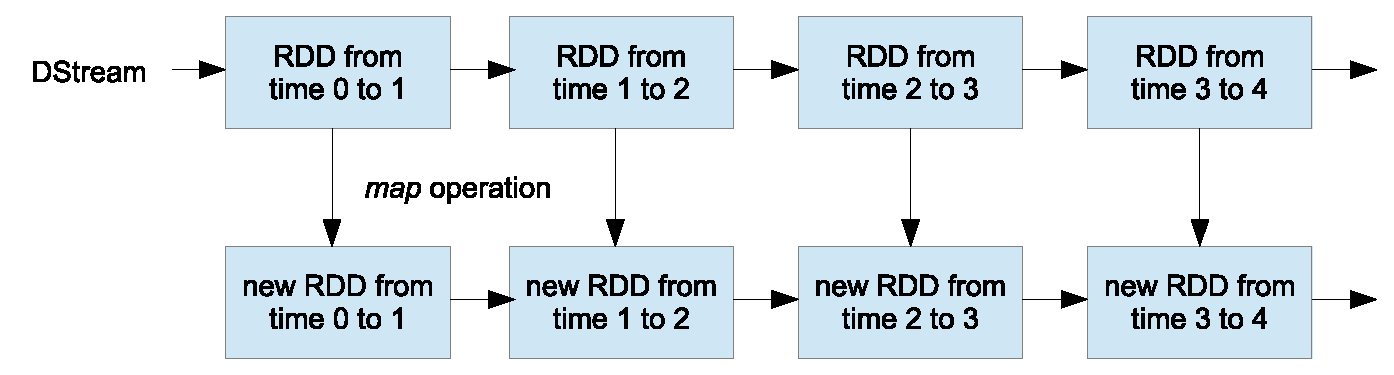
\includegraphics [width=1.0\textwidth]{images/DStreamWithTransformation}
  \caption{Transformation of a DStream to a new DStream.}
  \label{fig:DStreamWithTransformation}
\end{figure}

\textit{Input DStream} is a stream of raw data coming to Spark from the outer source.
Sources can be of two types: basic sources and advanced sources.
Basic sources are sources, that available using standard streaming context API, e.g. files or sockets.
Advanced sources are available using specific libraries, for example Kafka message queue server.
There is a notion of $Receiver$, that is an object that receives data from the stream, put into Spark's memory, so that it is available for input DStream, associated with this Receiver.
Every DStream is responsible only for one input data stream.
You can create many DStreams for different input streams to receive data from different data sources in parallel.
Receiver is executing as a long running task, hence it occupies one core of the processor.
This implies, that there should be more cores then receivers in the system.

Transformations on DStreams (UpdateStateByKey Operation, Transform Operation, Window Operations) ???

Spark streaming has a number of output operations on DStreams, that used to push transformed data to outer systems.
This can be files or databases.
Output operations actually start execution, as $actions$ of Spark engine do.
Examples of output operations are $print$, $saveAsObjectFiles$, $saveAsTextFiles$, $saveAsHadoopFiles$, $foreachRDD$.

DStream allows to persist it in the memory, when multiple computations of the same DStream are required.
Method $persist$ of DStream object does that.
Its execution specifies that every RDD of the DStream will be persisted in the memory, as it is done for RDD in Spark engine.
For data, arriving from network, the persistence level is so, that all data is replicated to two nodes to provide fault-tolerance.

There is a mechanism of checkpointing in Spark streaming.
It allows to make snapshots of intermediate data to HDFS.
It makes computation throughput less, if set not properly.
So it must be carefully tuned.

Fault-tolerance of Spark streaming is based on the fault-tolerance on Spark engine.
RDDs are basic elements of a DStream, what lets Spark streaming to rely on their robustness.
As long as all data locates on HDFS, if data node fails, all lost data can be recovered.
For data coming from network input stream, as we already mentioned, it is always replicated to two nodes.

\section{Auxiliary technologies}
% ������� 3 ����������� overview
\subsection{Avro [SP]}
\label{subs:avro}

Data should be structured when it is transferred over the network.
Data objects are converted into some form, in which they can be stored or transferred and later be reconstructed in a new environment.
This process is called serialization.
The naive serialization approaches are XML or JSON.
Drawback of these formats is that they require too much space for storing, because the data is kept it a text form.
The better solution is to use binary format for serialization and Apache Avro is one of the frameworks that use such approach.

Avro differs from the other serialization frameworks in that it does not require the code generation on receiving \cite{Avro1}.
It even allows to efficiently sort binary-encoded data without deserialization.
Also Avro supports easy schema changes, because it stores both old and new schemas and can associate fields with each other using their names.
This framework provides two types of encoding: binary encoding and using JSON.

Avro uses \textit{schemas} that are defined using JSON.
It needs a schema for serialization and in most cases this schema is transmitted along with the data.
Thus the receiving application does not need to store schemas for deserialization.
However, in some scenarios the transmission of schema is redundant, because both sides have the full schema stored locally.
In this case it is possible to transmit only a binary representation of serialized objects.

The schema can contain both primitive and complex types.
Primitive types include: \textit{null}, \textit{boolean}, \textit{bytes}, \textit{int}, \textit{long}, \textit{string}, \textit{float} and \textit{double}.
Complex types are: \textit{record}, \textit{array}, \textit{enum}, \textit{union}, \textit{map} and \textit{fixed}.
Listing~\ref{lis:example_avro_schema} illustrates the example schema.
One schema files stores only one schema definition.

\begin{lstlisting}[caption=Avro schema (example), label=lis:example_avro_schema]
{
  "name":"AppInstall",
  "namespace": "example.avro",
  "type":"record",
  "fields":[
     { "name":"id", "type":"long" },
     { "name":"userId", "type":"long" },
     { "name":"time", "type":"long" },
     { "name":"appName", "type":"string" },
     { "name":"packageName", "type":"string" }
  ]
}
\end{lstlisting}

Avro uses an \textit{object container format} for storing objects in a file.
A file has a specified schema, that consists of blocks with synchronization markers between them.
Blocks contain data objects and can be compressed.
Synchronization markers allow to split file for processing it with MapReduce.
Moreover, Avro file contains metadata section, where it stores a schema.

A file has the following structure: it has a header and one or several file data blocks.
The header contains information about encoding type and file metadata.
Metadata stores the schema and a type of codec that is used for compressing.
'null' codec type means that the data is uncompressed, 'deflate' codec uses the deflate algorithm.
The file data block stores information about the number of objects it contains, their sizes in bytes after compression, the serialized objects themselves and a synchronization marker.
This additional data helps to detect corrupted blocks.

Avro provides a \textit{Remote Procedure Call} (RPC) interface for implementing data exchange between a server and a client.
RPC protocol is defined using JSON.
Its attributes include a \textit{messages} object, that specifies the messages that are exchanged.  
\textit{Message} is a byte sequence, that is transmitted using a transport mechanism.
Transport system sends requests and receives responses.

Transport can have a stateless or stateful design.
\textit{Stateless} means that a server does not store any information about a client state.
The client transmits all the needed data in every request message.
In \textit{stateful} design the server keeps the persistent client state.
This approach has two problems.
First, the server should have a mechanism to discard client state at some point.
It is not possible to store the states of all the client for unlimited period of time.
Second, the server should be able to restore the client state in the case of the server crash.
This makes the process of server-side implementation complex comparing to sateless design.
However, stateful design results in better performance.
Figure~\ref{fig:stateful_stateless} represents the stateful and stateless schemas.

\begin{figure}
  \centering
  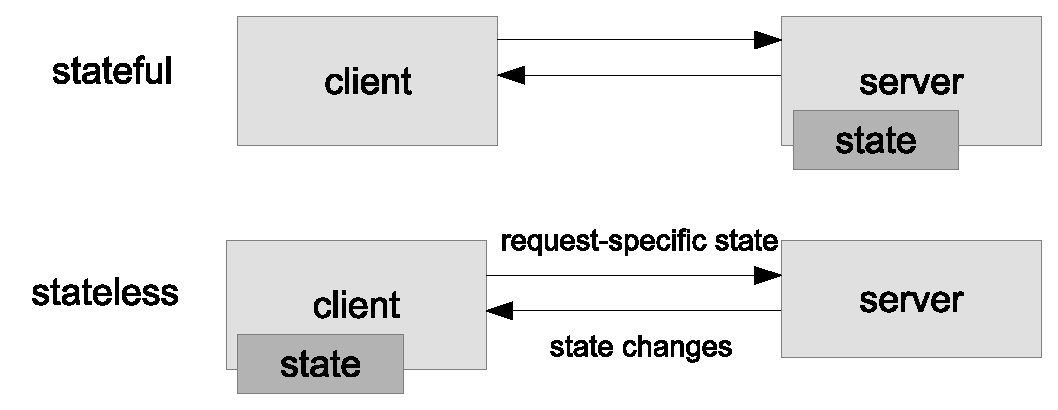
\includegraphics [width=0.7\textwidth]{images/stateful_stateless}
  \caption{Stateless and stateful design}
  \label{fig:stateful_stateless}
\end{figure}

An example of stateless transport method for Avro is HTTP.
In this case all Avro messages share the same URL at an HTTP server.
The 200 (OK) response code should be used by all response messages (normal and error).
Avro sends requests via the POST method.

There is an intermediate layer between messages and transport named \textit{framing}.
The main idea of framing is the partition of each message to a list of buffers.
A buffer contains buffer length followed by buffer data of this length.
Every message consists of one or several buffers.
Framing makes read and write operations more efficient.

Avro uses a handshake procedure before sending any RPC requests and responses.
It is used to make sure that the protocol definition is the same on both the server and the client side.
Only in this case the server and the client can correctly deserialize requests and responses.
To avoid extra network exchanges the server and the client stores recently used protocols in a cache.
Stateless and stateful transport differs in that the former requires a handshake before every request and response.
In contrast, the latter needs only one handshake and for the lifetime of the connection.

The handshake procedure is the following.
The client sends a \textit{HandshakeRequest} in a form \textit{(clientHash=clienthash, clientProtocol=null, serverHash=serverhash)}.
The \textit{clienthash} and the \textit{serverhash} are both the JSON protocol text, hashed with MD5.
The \textit{serverhash} contains data that the client received from the server during the last session.
If it is the first connection to this server the client tries to guess the server's hash.
The server sends in response a \textit{HandshakeResponse}.
If the received \textit{serverhash} is valid and the server knows the corresponding protocol to this client, the response has a form \textit{(match=BOTH, serverProtocol=null, serverHash=null)}.
In this case the connection is confirmed and the server can send a response message.
If the \textit{serverhash} is not valid, but the server knows the client protocol, it answers with \textit{(match=CLIENT, serverProtocol=serverprotocol, serverHash=serverhash)}.
It also allows the server to send the response data to the client.
However, the client must replace its nonvalid \textit{serverhash} data with that received from the server and process the response using the received protocol.
When the server is not aware of the client's protocol it received, it response with \textit{(match=NONE)}. 
Then the client re-sends its request extended by \textit{clientProtocol} value and the server response with \textit{(match=BOTH)}.

To determine the identity of the schemas stored on the client and the server side, Avro uses \textit{Parsing Canonical Form}.
It is a transformation, that removes data, irrelevant for the comparison, and normalizes the JSON text.
This canonical form can be used to create a fingerprint (an integer that serves as a unique id for a schema). 

 



\subsection{Scala}

\subsection{ZooKeeper [SP]}

Large distributed systems require a coordinator for system configuration management.
As it was mentioned in Chapter 4, Google uses a Chubby service for this purpose.
The main Chubby disadvantage is that for lock and unlock operations it is necessary to open and close the object consequently.
This feature influences the performance, increasing the time needed for making a lock.
Therefore Yahoo developes its own service named ZooKeeper that manages systems configuration and allows to efficiently lock the shared resources.

ZooKeeper namespace looks similar to a standard file system.
It consists of interconnected nodes, each of them identified by a path.
The path contains elements separated by a slash ('/').
Like in a file system, every node except the root has a parent node.
The parent node's path is a prefix for the current node path.
The ZooKeeper namespace differs from a standard file system in that its node can be a file and a directory simultaneously.

There are two types of nodes: persistent and ephemeral.
ZooKeeper stores persistent nodes on the disk, while ephemeral nodes belong to a particular session and exist only during this session.
Ephemeral nodes cannot have children nodes, they can only store data.
ZooKeeper client establishes a session with a ZooKeeper server, passing heartbeat messages.
When a client stopes to receive heartbeat messages, it reconnects to a defferent server, reestablishing the session.
If the session is canceled, all its ephemeral nodes are automatically removed.
ZooKeeper tree is presented in Figure~\ref{fig:zookeeper_tree} where the dark nodes are ephemeral.

\begin{figure}
  \centering
  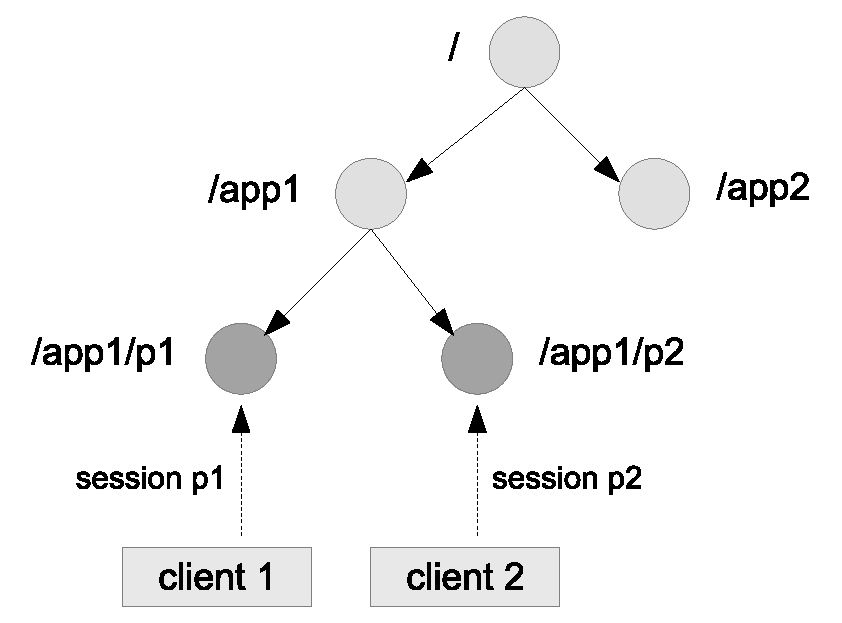
\includegraphics [width=0.5\textwidth]{images/zookeeper_tree}
  \caption{ZooKeeper tree sructure}
  \label{fig:zookeeper_tree}
\end{figure}

ZooKeeper is designed for small data warehousing, such as configuration, status and location information.
One node is usually not bigger than one kilobyte.
Therefore it stores data tree image in memory, keeping in a persistent store only transaction logs and snapshots.
In-memory storage limits the size of the database of ZooKeeper.
However, it gives advantages of low latency and high performance. 

The key feature of ZooKeeper is that it uses First In, First Out (FIFO) method for processing the messages.
It means that all commands are performed in the order they are received.
Thus, ZooKeeper maintains the total ordering.
The order is specified by a unique ZooKeeper Transaction id, that is assigned to each update.
 
ZooKeeper supports idempotent operations.
If a node should be updated, the system makes a note about the update and keeps an old and a new version of this node.
This allows client to receive the same message several times, being aware of when it can be applied.
Therefore all the write operations are performed sequentially in one thread and only on the master node.
On the contrary, read requests do not necessarily need the master node, they can be handled by a node's replica.

The client also supports the total ordering of the messages.
Hence if the client sends a write request and then a read request, the write operation is performed first.
Even if usually read operation does not need a lock, ZooKeeper strictly follows the order.
It allows to implement predictable asynchronous systems that work with ZooKeeper.

A client can watch a node.
If it sets a watch, it gets notified when the node is changed.
When the node sends this notification, it removes the watch.
In the case of connection problems between the client and the ZooKeeper server, the client receives a local notification.

ZooKeeper guarantees reliability using replication.
Its database is replicated to several nodes, one of them is a \textit{Leader} and the others are \textit{Followers}.
\textit{ZooKeeper Atomic Broadcast} (Zab) algorithm is used for managing the communication between the leader and the followers.
It synchronizes the replicas, broadcasts updates and recovers the valid state in the case of nodes crash.

Zab includes four phases: (1) Leader election, (2) Discovery, (3) Synchronization and (4) Broadcast.

1. On the first stage ZooKeeper uses any election algorithm to choose a leader.
After termination every node stores its vote locally in volatile memory.
When a node \textit{n} votes for a node \textit{n'}, \textit{n'} becomes a \textit{prospective leader} for \textit{n}.

2. On the second stage the nodes inform the prospective leader about the most recent transactions they accepted.
Thus the prospective leader knows the latest sequence af accepted transactions and can establish a new epoch.
From thit moment the previous leaders cannot perform any commits.
In the case of connection problems between a follower and a leader, the follower goes back to the stage (1) of this algorithm.

3. The leader is aware of the latests transactions history and during this stage synchronizes this information with its replicas.
This phase is also called voting phase, because it receives the votes from the nodes.
The leader performes a commit only if it receives acknowledgements from two of three followers.
At this moment the leader changes its state from \textit{prospective} to \textit{established}.

4. The nodes persist in this stage until a crash.
Every write request from a ZooKeeper client is broadcasted among the nodes.
New followers can join, receiving the transaction history from the leader.
The leader and its followers use periodic heartbeat messages for early failure detection.
If any of the nodes does nor receive a heartbeat message within a timeout, it shifts its state to \textit{election} and goes back to the first stage.

It can happened that one of the followers still has an outdated information when it receives the read request.
To avoid this problem, it is possible to make a force synchronisation with the master.
It is called the \textit{slow read}.
Evidently, if all the clients use the slow read the system looses the advantage of scaling.
Without force synchronisation ZooKeeper system scales for reads nicely. 
However, in this case the client that reads from a replica can obtain the outdated information.

\subsection{Kafka [SP]}

The straightforward way to store user activity tracking data is to use a logging service.
It collects data, formes batches and stores them in a file system.
However, this approach does not provide a real-time access to stored information.
System that needs to handle real-time data cannot be content with batch-oriented mechanism.
It requires a pipeline that can transfer data between the system components without considerable delays.
Therefore a publish-subscribe mechanism named Kafka was invented by LinkedIn.

Kafka is a message broker that can deliver thousands messages per second. 
It provides high throughput and low latency of data handling.
It is built as a write-ahead log.
Data producers write data into a persistent store and data consumers read these records.
The Kafka structure is illustrated in Figure~\ref{fig:kafka_structure}.

The time of retaining a message is configurable.
The message is kept for a particular period of time, when it is available for consumption.
Then it is removed to free up space.

\begin{figure}[h]
  \centering
  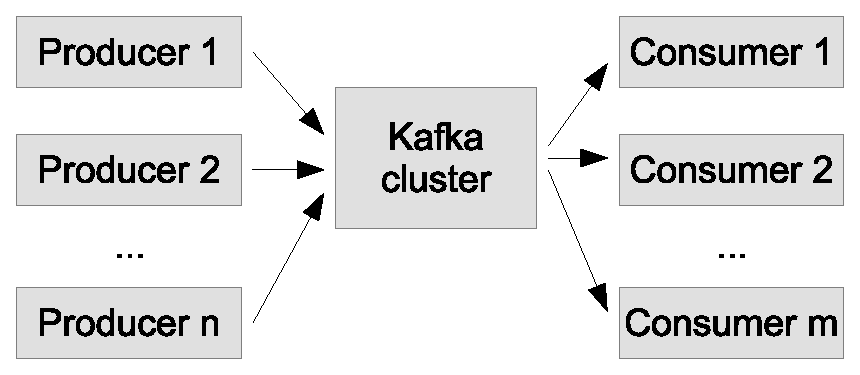
\includegraphics [width=0.5\textwidth]{images/kafka_structure}
  \caption{Kafka structure}
  \label{fig:kafka_structure}
\end{figure} 

\mnote{Kafka topic}
The core abstraction in Kafka is \textit{topic}.
One topic aggregates messages of one type.
For example, the system tracks the user activity, e.g. the number of times he opened a particular application or visited a particular website.
All these records are stored in the topic 'User activity'.
It is recommended to have a small number of topics (no more than a thousand).
However, each topic can contain  billions of messages.

One topic is a log that is spread over a cluster of brokers.
Every Kafka broker consists of zero or more partitions.
Figure~\ref{fig:kafka_topic_structure} illustrates the topic structure.
Kafka continually appends messages to the partitions.
Each partition represents an ordered sequence of messages that are uniquely identified by ids.
This id is called the \textit{offset}.
The sequence of messages is immutable and can only be extended by addition of new messages.
Besides appending, system provides one more operation: messages fetching.
Messages can be obtained from a particular partition, if a beginning message id is specified.
Kafka has an API for these operations, that can be used in different programming languages.

To provide fault tolerance, Kafka replicates each partition across several servers in a Kafka cluster.
One of these servers is a 'leader' and others are 'followers'.
The leader is responsible for handling all read and write requests.
The followers only replicate the leader.
For load balancing each server is simuntaneously a leader and a follower, i.e. for some of its partitions it acts as a leader and for others - as a follower.

The follower acts as a normal consumer, receiving data from the leader and applying it to its log.
Only when all the replicas received the message it is considered to be 'committed' and can be delivered to real consumers.
This guarantees that no message is lost even in the case of the leader failure.
A consumer always receives a message that is committed to the Kafka cluster.
A producer can wait until the message is committed or not, depending on the application logic.

To choose the leader, Kafka maintains a dynamic set of in-sync replicas (ISR).
Only these replicas can participate in the leader elections.
All these nodes must receive a message to consider it to be a committed write.
ZooKeeper stores the ISR set and tracks every change of its membership.
When a Kafka cluster has \textit{n}+1 replicas, it can sustain \textit{n} failures without any problems.

% �������� �������� ��� ��� � ������� ������ ����� ��� ���
%[reference: http://kafka.apache.org/documentation.html]
\begin{figure}[h]
  \centering
  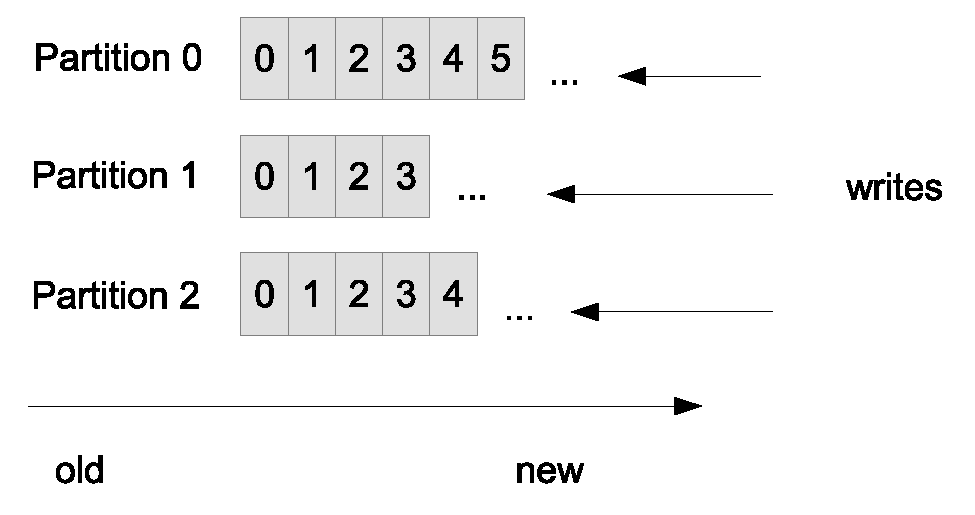
\includegraphics [width=0.5\textwidth]{images/kafka_topic_structure}
  \caption{Kafka topic structure}
  \label{fig:kafka_topic_structure}
\end{figure} 

Kafka uses a publish/subscribe mechanism to establish a communication process between producers and consumers of data.
One subscriber consists of a group of processes that run as a cluster.
Only one machine in this cluster obtains messages from Kafka.
Moreover, it consumes data from a specified partition.
Therefore, the subscriber parallelism depends on the number of partitions of the topic.
Kafka uses ZooKeeper to add or remove nodes from the broker and consumer groups.
It helps to rebalance the load automatically.

The fact that each partition has only one consumer makes it easier to store the metadata about what has been already consumed.
The consumer process just needs to store the last acknowledged message id.
Kafka uses 'at-least-once' semantic for message delivery.
It means that if the cunsumer process crashes, it reprocesses some messages from its partition one more time. 

There are two ways to balance load over Kafka brokers for message producers.
On the one hand, it can be done randomly.
On the other hand, application can supply a key that can be used to hash messages for partitioning.
The latter way guarantees the order of messages between partitions, that is not provided by Kafka.
Also it helps distributed consumers to make in-process aggregation.
In this case a consumer can obtain data from a particular partition, knowing that it contains a part of information it needs.  

For enhancing throughput Kafka introduces three techniques. 
First, it partitions data to production, consumption and brokering parts.
Second, it batches messages to chunks to send them together.
Third, it shrinks the data to decrease the amount of data that should be sent.

\mnote{batching}
The Kafka producer can send messages in synchronous or asynchronous ways.
In asynchronous mode small messages are collected into batches.
This allows to send data in chunks over the network. 
As it is done on application level, it is possible to control the batch size and the maximum time of holding the message.
Kafka allows to group messages from low-volume topics and high-volume topics together, reducing the amount of small requests.
On the filesystem level the mechanism of pagecache is used to buffer writes.
Kafka allows to delay the flush to disk again on the application level.
Similarly, it gives a control over the message boudaries and makes possible to have different policy for different topics.
Batching is also useful on the consumer side.
The client specifies the starting message id and the maximum buffer size it can receive at one time.
Kafka provides a possibility to combine data from several topics in one request.

\mnote{shrinking}
There are two techniques of data shrinking: via serialization and via compression.
Kafka associates schemas with the topics to extract the repeated structure from the messages.
Along with serialization, these schemas can be used to provide the compatibility and integration facilities.
The popular software that is used in combination with Kafka for serialization is Apache Avro.
It is described in details later in this chapter.
Kafka is able to compress several messages into a composite set of messages.
This is done during the batching process of the Kafka producer.
Thus, the messages in the compressed form are transferred to Kafka, where thay are stored and handled also in a compressed form. 

As the data transferred through Kafka is very diverse, a uniform schema is used for every topic.
This schema is kept all the way, from Kafka producer to Kafka consumer.
The schema usage is mandatory and is automatically checked.
As the schema sometimes changes, Kafka stores all its verions.
Each message contains a schema version id with which it was created.
Every schema is thoroughly tested when registered to detect incompatibilities in a timely manner.

\mnote{system monitoring}
A special Kafka topic exists to detect the percentage of data loss.
It audits the number of messages that are sent and received within a given topic over a specified period of time.
For this purpose each producer and consumer periodically notifies the audit topic about the number of processed messages.
The timestamps are extracted from the messages, instead of using the machine time of the message processing.
It is done to deal with delays in message delivering.
Kafka provides a standalone application for monitoring that processes the data from the audit topic.
It computes the ratio of data loss and duplication and is able to produce alert messages.

Kafka can by applied in a number of ways.
First, it can serve as a message broker, allowing to separate data producers from data processing.
Second, it provides facilities for real-time monitoring.
For instance, Kafka can be used to monitor the website users activity or to aggregate some application statistical data.
Third, it can serve as a log aggregation system, that can operate a log messages stream instead of dealing with log files.
This approach decreases latency and makes easier log data collection from several sources.

\mnote{log compaction}
One more Kafka application is a distributed system commit-log, that is used for restoring the failed nodes.
For this purpose Kafka has a specific feature - a \textit{log compaction}.
The main idea of log compaction is that Kafka guarantees that for all the message keys it retains the last known value.
The simpler data retention approaches are time- or size-based.
For example, Kafka removes the log data that is older than a specified period of time.
In this case some values that change rarely can be lost.
On the contrary, log compaction guarantees that at least the last value for each key persists.
This allows to fully restore the state of the broken node.

Another property of log compaction is that it shrinks the log size, removing the old records.
Using the complete log of all changes system can restore its state to any point by re-processing all the changes from the beginning of the log.
However, this approach requires a lot of memory for storing all the changes that leads to poor performance.
Log compaction removes only those records where more recent updates with the same key exist. 
Due to this fact the exterior system does not need to read the whole log and replay all the changes in order to restore its state.
Each topic has its own retention policy, i.e. one cluster can combine time or size retention with log compaction retention.

%[reference: http://kafka.apache.org/documentation.html#majordesignelements]
Figure~\ref{fig:kafka_log_structure} presents the Kafka log structure. 
The head of the log has a sequential numeration (offset) and retains all messages.
The tail of the log has a compacted structure, that contains only selected records.
It is important to mention that the messages in the log tail keep the original offset.
Kafka assignes this offset only once when a message is written for the first time and never changes it.
Moreover, even offsets for removed records are still valid log positions.
In this case Kafka returns the next highest existing value.
For instance, in our case requests with offsets 14, 15, 16 and 17 all return data starting from 17.

\begin{figure}[h]
  \centering
  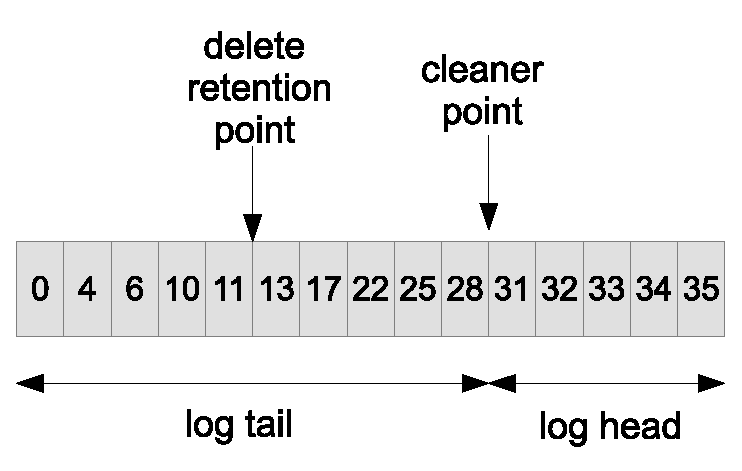
\includegraphics [width=0.5\textwidth]{images/kafka_log_structure}
  \caption{Kafka log structure}
  \label{fig:kafka_log_structure}
\end{figure} 

Compaction also performs message deletions.
If the message is marked to be deleted, all its previous versions (records with the same key) will be removed.
Deletion markers are not retained in the log after 'delete retention point' presented on the picture.

Log compaction is a background process that is run periodically.
Figure~\ref{fig:log_compaction_process} visualises a simple example.
Log compaction process posesses the following properties:
first, it guarantees the messages ordering even after compaction.
Second, the message offset is immutable and serves as a position of the record in the log.
Third, a read operation returns at least the final version for each value associated with a key.

\begin{figure}[h]
  \centering
  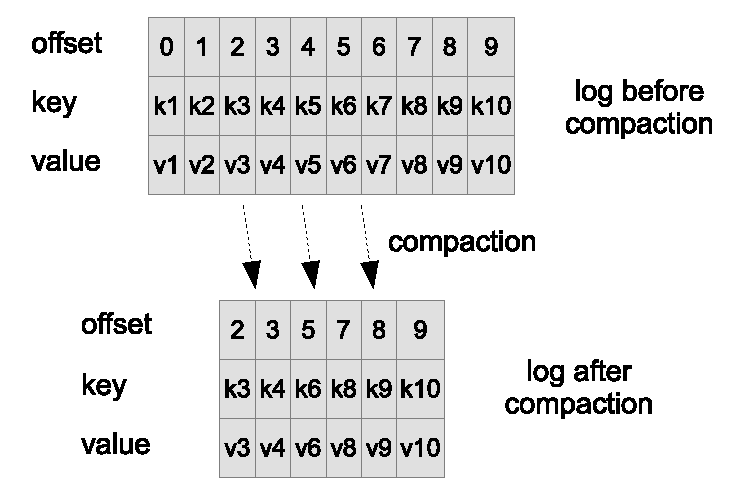
\includegraphics [width=0.6\textwidth]{images/log_compaction_process}
  \caption{Kafka log structure}
  \label{fig:log_compaction_process}
\end{figure} 

The compaction process consists of the following steps:
(1) The log is chosen, that has the biggest number of records from log head to log tail.
(2) For each key in the log head compaction process determines the last offset.
(3) The log is copied from the beginning to the end, removing the keys that occure later in the log. 
   




\section{Alternatives}

\subsection{Cassandra [VI]}
\label{subs:cassandra}

Cassandra is a distributed storage system \cite{Cassandra, Avinash2014, Hewitt2011}.
It is efficient and reliable, what is achieved via multinode topology and replication of data.
It keeps data on many commodity machines without having master node.
This leads to a purely distributed approach, where there is no a single point of a failure.
Cassandra is highly scalable, as long as any number of nodes can be added to the cluster at any time.
It provides CQL language, that allows writing and querying data in an SQL-style manner.

Cassandra's architecture is purely distributed.
It consists of a set of nodes, and all of them are equal in the sense of functionality.
Each node stores the part of data, what allows to extend capacity of the storage, basically, to any size.
Nodes exchange meta-information about the cluster's structure once per second.
Every node maintains a \textit{commit log} of writes.
Then it saves all written data to an in-memory data structure called \textit{memtable}, that functions as a cash.
When memtable is full, node flushes it to an SSTable file, partitioning and replicating data among the cluster.
Cassandra allows to connect to any node in the cluster, that works then as a coordinator.
It routs then requests of the client to nodes that have requested data.

\mnote{Main structures}
There are 5 main structures in Cassandra, that need to be defined.
\textit{Cluster} is a set of nodes that store the data.
\textit{Data center} is a subset of cluster's nodes that are grouped together.
They have a common configuration to achieve optimal replication and segregation properties.
Data still can be copied to several data centers, if replication factor is high.
\textit{Commit log} is a local storage on each node, where data is stored for durability, before being distributed across the cluster.
\textit{Table} is a logical place, where data is stored.
It is, essentially, a set of columns, that can be accessed by rows.
Each row has a primary key and a value, represented by a particular set of columns, that need not be the same for every row in the table.
\textit{SSTable} (sorted string table) is a file, where node periodically writes data, gathered to a memtable.
It is immutable, append-only, and exists for every Cassandra's table.

\mnote{Communication between nodes}
For communication between nodes Cassandra has a protocol called \textit{gossip}.
It allows to discover information about other nodes in the cluster, and to share information about state of the node.
According to gossip protocol every node communicates with three other nodes every second, exchanging meta-information about state, data, and other nodes.
Such network learns fast about its topology and state.

\mnote{Detection of failures and recovery}
Cassandra analyses state of nodes using gossip information to check whether node is up or down.
It tries whenever possible not to send any requests to nodes, that are out of service by any reason.
Particular node tries to understand, which other nodes are down directly, by communicating with them, as well as indirectly, receiving information about them from directly communicated nodes.
Node can fail due to many different reasons, e.g. hardware failures, software crashes, or network outages.
Cassandra does not remove the node from topology as soon as it seems to be down.
Instead, nodes try to re-establish communication with failed node.
It can be smart, because, for example, a network outgage can be recovered fast.
As long as node detected to be failed, other nodes start to replicate data bypassing it.
Administrator has to run a repairing tool, after node is up, to make it again consistent with the cluster.

\mnote{Data distribution}
Data distribution and replication are inherent properties of Cassandra.
Data is stored in tables, that consist of rows.
Row is an atomic peace of data in Cassandra.
It has a primary key, that defines its location in the cluster.
There are four aspects, that determine distribution and replication: virtual nodes, partitioners, replication strategies and snitches.
We discuss them shortly in details.

\mnote{Consistent hashing}
First, let us describe consistent hashing.
It divides possible values of partition keys into ranges.
Partition key is any column name of a row.
This allows to set for each node a subset of partition key values, that will be stored in this node.
Consistent hashing has an advantage, that it minimizes reorganization needs, when nodes are removed or added.
For a particular partition key, consistent hashing produces for each node an interval of hash-values.
Then for a new row, it is stored on the node, so that hash-value of key maps to the interval assigned to this node.

%Virtual nodes

\mnote{Data replication}
When new row is added, Cassandra replicates it across the cluster.
Copies of the row are called replicas.
Each replica is equal to others, and there is no any master or primary replica.
The number of replicas is called a \textit{replication factor}.
It defines on how many nodes replicas of a row will reside.
There are two strategies of a replication mechanism.
The first one is a \lstinline{SimpleStrategy}, that supposes to use only one data center for replication.
Another one is a \lstinline{NetworkTopologyStrategy}, that is used in most cases, and allows to replicate data across the whole cluster.

\mnote{Partitioners}
Now let us describe what is \textit{Partitioner}.
Partitioner defines how data is distributed across the cluster.
It computes a token from a partition key of a row.
This token is then used to choose nodes, where replicas of a row must be saved.
There are three partitioners in Cassandra: \lstinline{Murmur3Partitioner}, \lstinline{RandomPartitioner} and \lstinline{ByteOrderedPartitioner}.
\lstinline{Murmur3Partitioner} distributes data uniformly in the cluster using \lstinline{MurmurHash} hash function.
\lstinline{RandomPartitioner} distributed data uniformly using \lstinline{MD5} hash function.
\lstinline{ByteOrderedPartitioner} distributes data in a lexical order by key bytes.

\mnote{Snitches}
Snitches define mapping of nodes to data centers and racks.
Using snitches Cassandra understands how to route requests.
They provide topology information and allow to execute replications properly.
Snitch monitors historical information about efficiency of reading from different replicas of a row, and uses this information to choose the best one for a request.

When a client connects to Cassandra, it is able to communicate with any node. 
Requests are then redirected by a connected node to the one, that has a particular data to be returned to a client or to be written.
Connected node is called \textit{coordinator}.
Coordinator is, essentially, a proxy between a client and Cassandra store.

\mnote{CQL}
Cassandra has a query language \textit{CQL} (Cassandra query language).
It is an interface to communicate with Cassandra, to read and write data.
It is an SQL-style language, that allows to query data from Cassandra with different conditions.
As SQL it is based on a table representation of data.

\subsection{RabbitMQ [VI]}

RabbitMQ is a queue messaging server \cite{RabbitMQ, AlvaroWilliams2012}.
It provides a robust, efficient and scalable message broker, that serves as an intermediate layer between publishing and subscribed clients.
RabbitMQ has a simple data model, that nevertheless offers a flexibility in the structure of data flows.
It gives an opportunity to adjust a tradeoff between throughput and reliability.
RabbitMQ fully applies Advanced Message Queuing Protocol (AMQP).

General structure of RabbitMQ
Producers
Consumers
Brokers
AMQP connection and channels

\textit{Advanced Message Queuing Protocol} \mnote{Advanced Message Queuing Protocol (AMQP)} or \textit{AMQP} is something \cite{AMQP2011}.

Queues

Exchanges and bindings
Routing key and exchange type
Direct
Fanout
Topic

Virtual hosts and separation

Durability
Delivery mode - persistent
Durable exchange
Durable queue

Delivery verification

\subsection{Thrift [VI]}

Description of Thrift \cite{Slee2007} \cite{Thrift}.


\chapter{The Menthal Speed Layer}
\label{chap:menthal_backend_architecture}

TODO: introduction

\input{content/08-Menthal_backend_architecture(Requirements_analysis)}

\section{Design of the system [VI]}
Architecture - general schema (picture)
9 pages

General architecture as a speed layer.

Figure~\ref{fig:SpeedLayerArchitecture}

\begin{figure}[h]
  \centering
  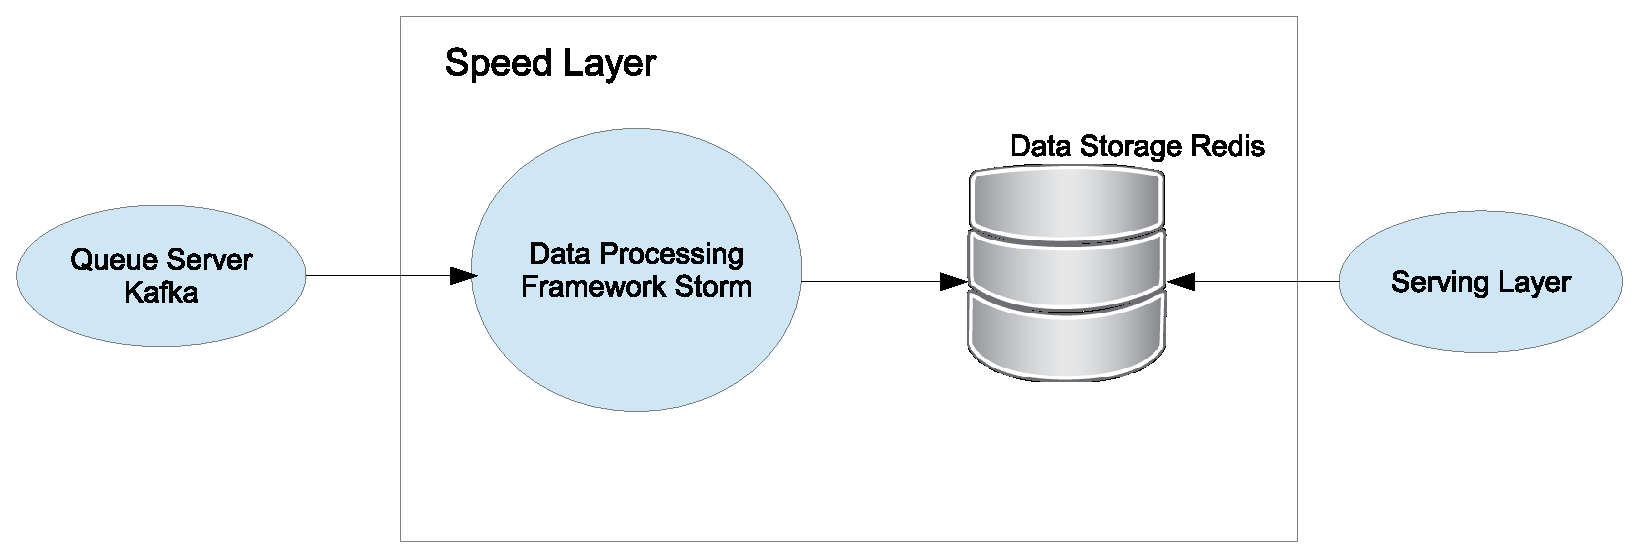
\includegraphics [width=1.0\textwidth]{images/SpeedLayerArchitecture}
  \caption{General structure of the Speed Layer.}
  \label{fig:SpeedLayerArchitecture}
\end{figure}

one paragraph for each part: source, processing, storage

\subsection{Data source}
kafka
topics and spouts for each event type

\subsection{Data processing}
storm
topology
bolts
events
aggragations
anomaly detection
classes

\subsection{Data storage}
redis
keys
access to redis
transactions and pipelining

\section{Use Cases [SP]}
\label{sec:use_cases}

This section presents two examples of using the Speed layer architecture, described above.
The main purpose of the Speed layer is to process the incoming events.
In the context of the Menthal project we need to calculate various aggregations.
In addition, our project allows to perform anomaly detection analysis.
These features are described in more detail below.

\subsection{Aggregations}

In our project we use two types of aggregations: user-based and application-based.
Table~\ref{fig:user_based_aggregations} represents the table of user-based aggregations.
Each of these aggregations is calculated with different granularities: hourly, daily, weekly and monthly.

\begin{table}
  \centering
  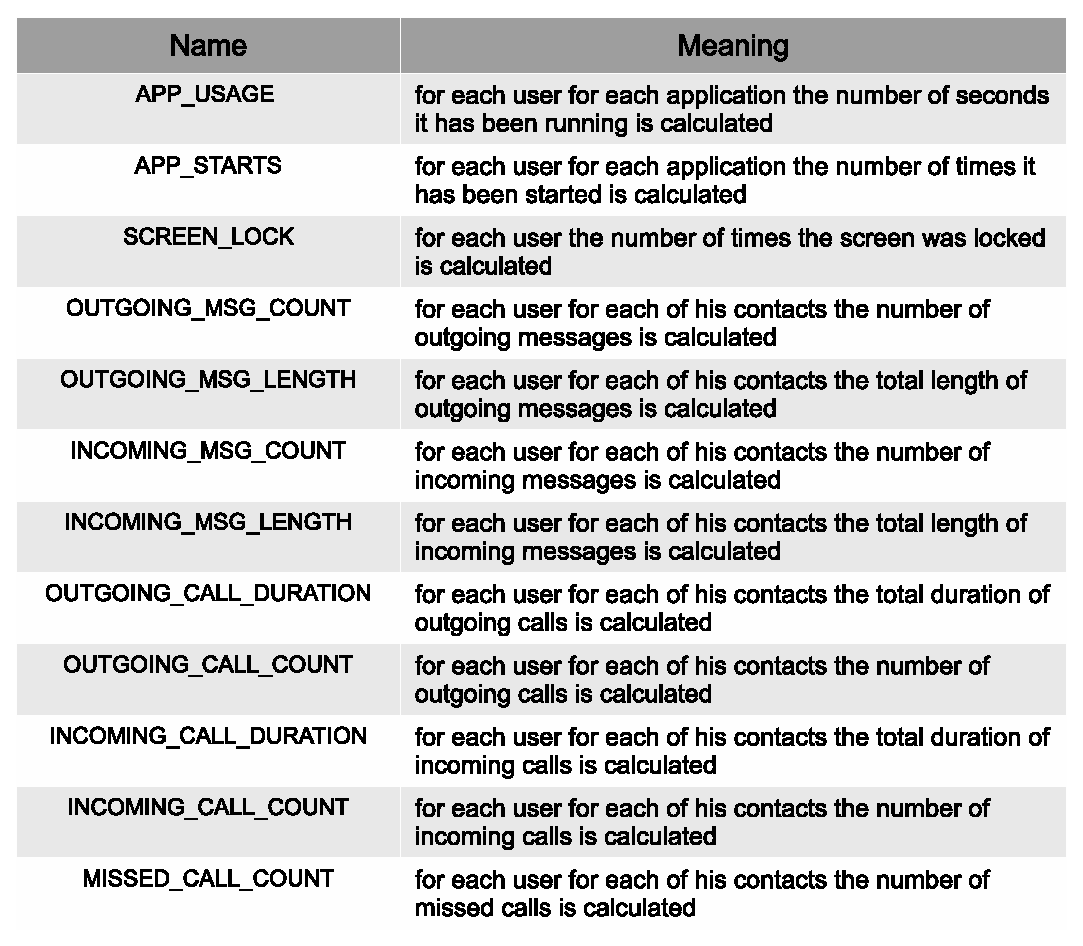
\includegraphics [width=1.0\textwidth]{images/user_based_aggregations}
  \caption{User-based aggregations}
  \label{fig:user_based_aggregations}
\end{table}

The aggregations presented in the table are made for each user separately.
However, all these aggregations except SCREEN\_LOCK are also implemented as a sum and average for all users. 
Another group of aggregations is global summaries for different applications.
We calculate for each application the number of unique users, the number of sessions and total time spent. 

The implementation of aggregations in our case is based on Redis.
There is an interface \textit{EventAggregator} that actually allows to use any other data storages.
However, in our work we concentrate on Redis implementation of this interface.
It perfectly fits our needs for fast access and this storage is easy to use and does not need a lot of programming effort.

\subsection{Anomaly Detection}

People download various applications for their smartphones and do not pay much attention to the questions of security.
There is a risk that applications from unofficial stores contain the malicious software.
Moreover, the software from an official store can turn out to be infected.
The main problem is that usually users do not read what personal information the application requests an access to.
And even if they read it, they do not have a choice to give the permissions or not.
Without giving the required access rights, a user cannot install this application on the smartphone.
   
The malicious software on smartphones behaves in different ways.
It can try to spread and infect all the contacts in a user's contact list.
For instance, a virus can send an sms, that contains its copy.
The virus can download and install another malicious software on the user's smartphone.
To apply some changes that the virus has performed in the system, it can restart the device.
Sometimes the malicious software can even make calls to specific numbers, so the user is charged for them.

\mnote{anomaly type}
As it was mentioned in section \ref{sec:anomaly_detection_algorithms}, there are a lot of ways to detect anomaly in incoming data.
Let us first decide what kind of anomaly we are dealing with.
Usually users do not have a strict pattern of interacting with their smartphones.
The sequence of performed actions changes from time to time.
One day a user can start with a phone call, another day by sending several messages.
This means that our anomaly is not \textit{collective}.
We consider a data instance independently from neighboring instances, therefore the anomaly type is not \textit{contextual}.
Thus we can conclude that we are dealing with the \textit{point} anomaly.

\mnote{anomaly detection approach}
Next step is to decide what approach to use for point anomaly detection.
The percentage of infected smartphones among the Menthal users is low.
It happens because the Android platform has good protection mechanisms and the official application stores are regularly tested for viruses.
Therefore we have a lot of \textit{normal} data and it is hard to get \textit{abnormal} examples (data from infected phones).
In this situation we cannot use supervised learning, so we have chosen an unsupervised approach.

\mnote{One-class SVM}
There are several anomaly detection techniques that implement an unsupervised approach.
We decided to use one-class support vector machines (SVM) technique, because it perfectly fits our demands.
First, it needs only 'normal' data instances for learning.
Also it can work with high-dimension data, i.e. when a feature vector consists of more than two features (we need four in our case).
Moreover, there is an existing java library called libsvm \cite{libsvm} that among other techniques implements one-class SVM.

Follow the assumed malicious software behavior, we try to detect the suspicious behavior of the smartphone.
For this purpose we analyze four events that are received from the clients: \textit{sms\_sent}, \textit{app\_install}, \textit{phone\_shutdown} and \textit{call\_outgoing}.
For simplicity we only count the number of these events.
However there is a possibility to make more thoughtful research, using the values that these events contain.
For example, traffic data, namely the number of transferred bytes, can be used for analysis.
To have a basis for comparing the amount of events, we use a time window.
In other words, for each type of event we calculate the number of times it occurs in a specified time interval (one hour by default).
Roughly speaking, we can take the number of times the event occurs in a normal state, than calculate this number for an unknown state and make a conclusion whether it is normal or abnormal.

To use One-class SVM algorithm we need to create a training data set.
When the training set is ready we run \textit{svm\_train} method to create a model.
Then we use \textit{svm\_save\_model} method to safe the trained model, so it can be used later for anomaly detection.

\mnote{flow of events}
The Speed Layer has the following architecture to allow anomaly detection of incoming data.
Figure~\ref{fig:anomaly_detection_data_flow} illustrates the data flow.

\begin{figure}[h]
  \centering
  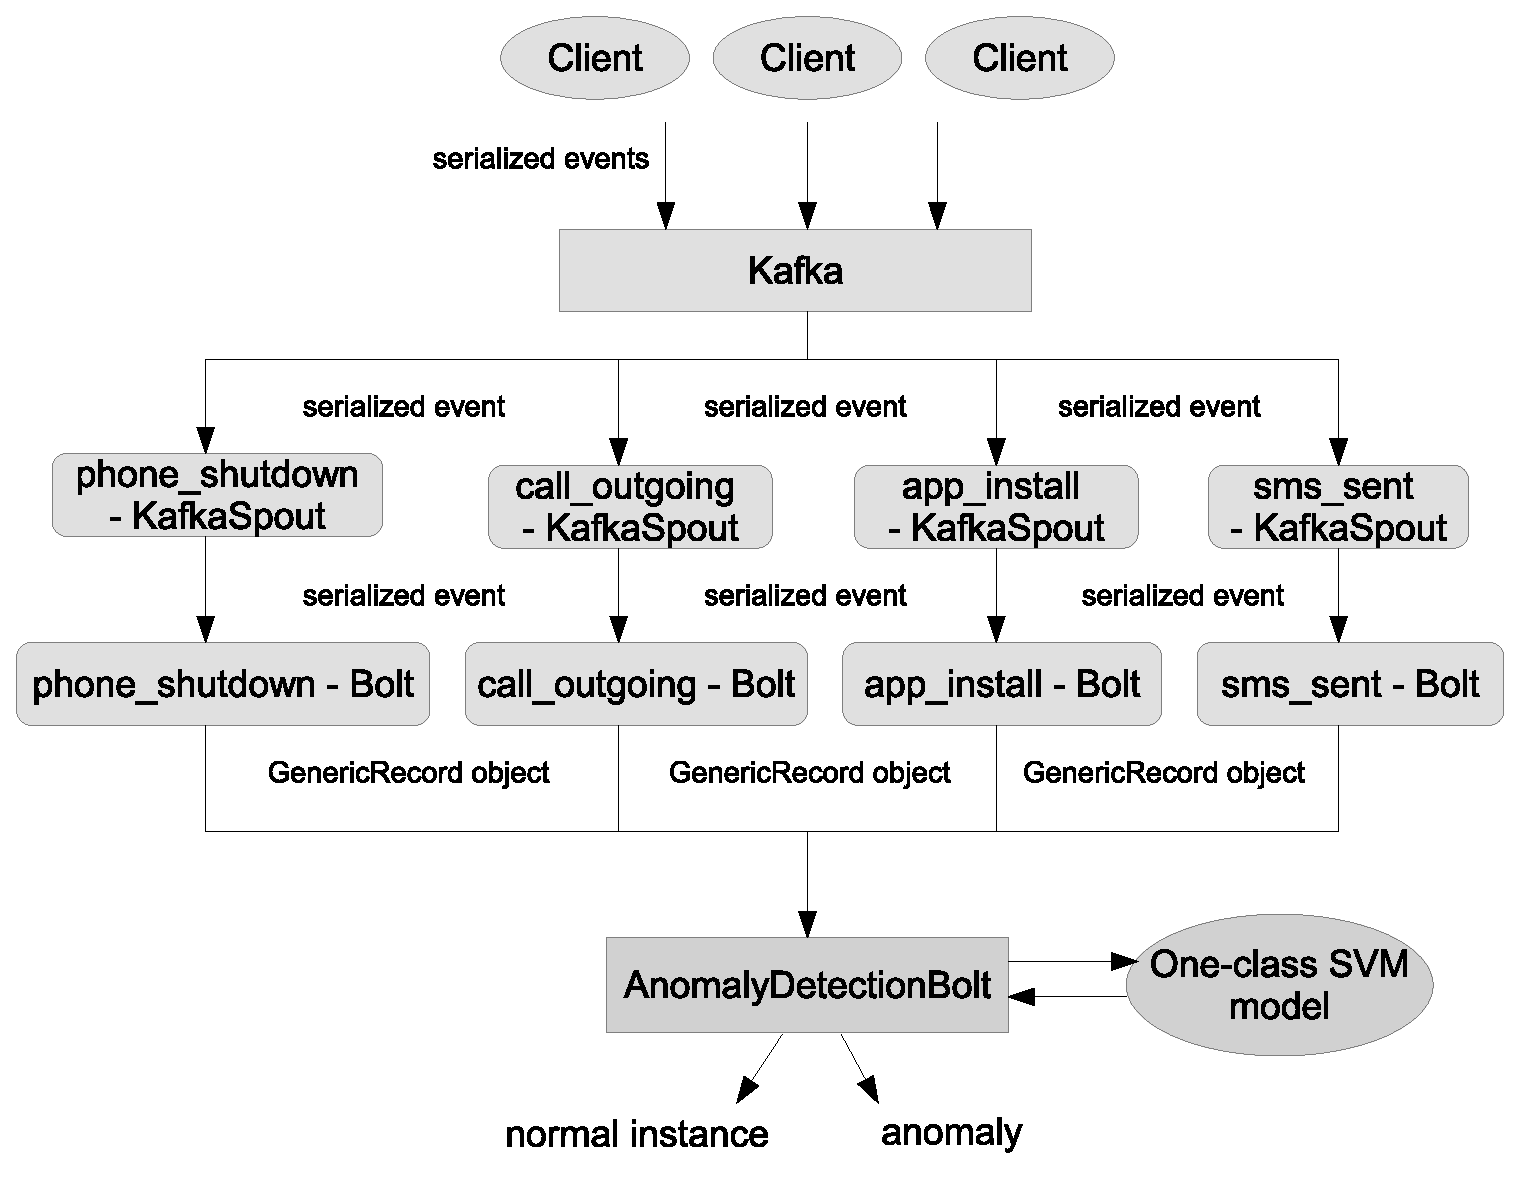
\includegraphics [width=1.0\textwidth]{images/anomaly_detection_data_flow}
  \caption{Anomaly detection: data flow}
  \label{fig:anomaly_detection_data_flow}
\end{figure}

For each Kafka topic a separate KafkaSpout receives messages.
One message contains the description of a particular event that happened on the client side (e.g. sms\_sent).
For each event type a separate bolt receives data from a corresponding KafkaSpout.
Then the bolt deserializes the received message, creating a \textit{GenericRecord} that represents the event.
For the events that are interesting for anomaly detection, there is an additional step.
Bolts, that receive data of type \textit{sms\_sent}, \textit{app\_install}, \textit{phone\_shutdown} and \textit{call\_outgoing}, emit the created GenericRecords to an \textit{AnomalyDetectionBolt}.

\mnote{Anomaly Detection bolt}
The main function of AnomalyDetectionBolt is to form data instances from incoming events.
As our version of Speed layer uses Redis as a data store, AnomalyDetectionBolt also uses it to accumulate events.
When a new event is received, AnomalyDetectionBolt extracts a type of event, a user id, and time when this event occurred.
Using the user id, the bolt requests the value of \textit{lastCheckTime} that is stored in Redis.
The \textit{lastCheckTime} value is compared with the time, extracted from the received event.
If the time delta is bigger than a specified threshold, the new check for anomaly is performed.
The frequency of anomaly checks is regulated by an ANOMALY\_CHECK\_INTERVAL parameter.
This mechanism sets only one-side bound, so the check is performed not more than every half an hour by default.
However, if the bolt rare receives events from a particular user, the check for anomaly is run with the same low frequency. 

AnomalyDetectionBolt uses a sliding window to accumulate events.
The size of the window is regulated by a TTL parameter.
TTL specifies how long the event is stored in Redis.
Each time the new check for anomaly is performed, the bolt first of all deletes all outdated events from the store.
This guarantees that the data instance that participates in anomaly detection contains events that are collected over a specified period.
For example, the size of the sliding window is one hour by default.
If we want to perform an anomaly detection analysis, we take the mentioned earlier four types of events and count how many times each of them has occurred during the last hour.
Using this numbers the bolt forms a data instance.  
Then it checks whether the instance is an anomaly or not using the trained one-class SVM model.

To get correct results it is essential to select the optimal parameters for One-class SVM.
Table~\ref{fig:svm_parameters} represents the parameters, their meaning and values that are optimal for our case.
The process of parameters selection includes a technique called \textit{cross-validation}.
Here the data set is divided into two parts - training set and testing set.
This helps to avoid the problem of model overfitting.  

\begin{table}[h]
  \centering
  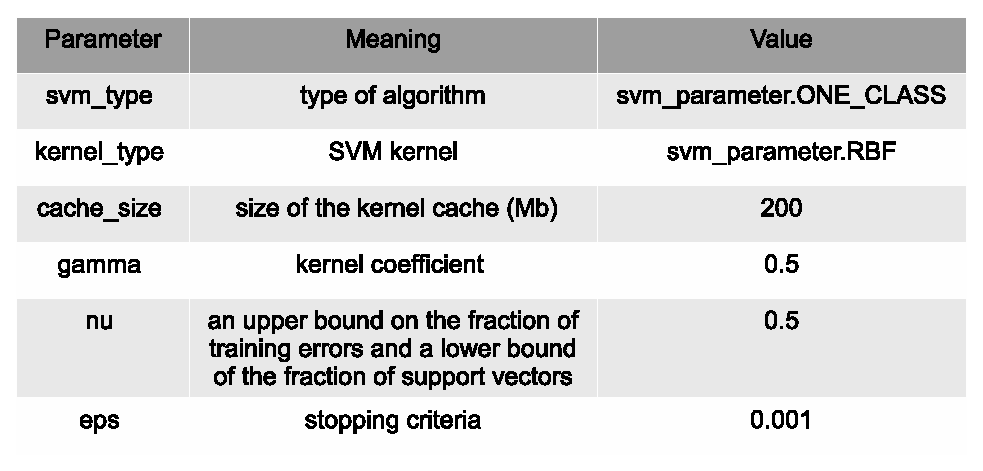
\includegraphics [width=0.9\textwidth]{images/svm_parameters}
  \caption{One-class SVM parameters}
  \label{fig:svm_parameters}
\end{table}







 	

 
 


%\section{Data flow}
%General schema (picture)
%3 pages

%\section{Algorithms}

%\section{Mapping to hardware}
%how many servers, characteristics, data transferring
%1 page

%\section{Aspects of implementation}
%programming languages, etc.

\chapter{Implementation}
\label{chap:implementation}

% rename chapter to Use cases

% first paragraph:
% architecture was described
% now we show how to use it
% two examples
% one subsection about aggregations
% one subsection about anomaly detection

Aggregations

In our project we use two types of aggregations: user-based and application-based.
Figure~\ref{fig:user_based_aggregations} represents the table of user-based aggregations.
Each of these aggregations is calculated with different granularities: hourly, daily, weekly and monthly.

\begin{figure}
  \centering
  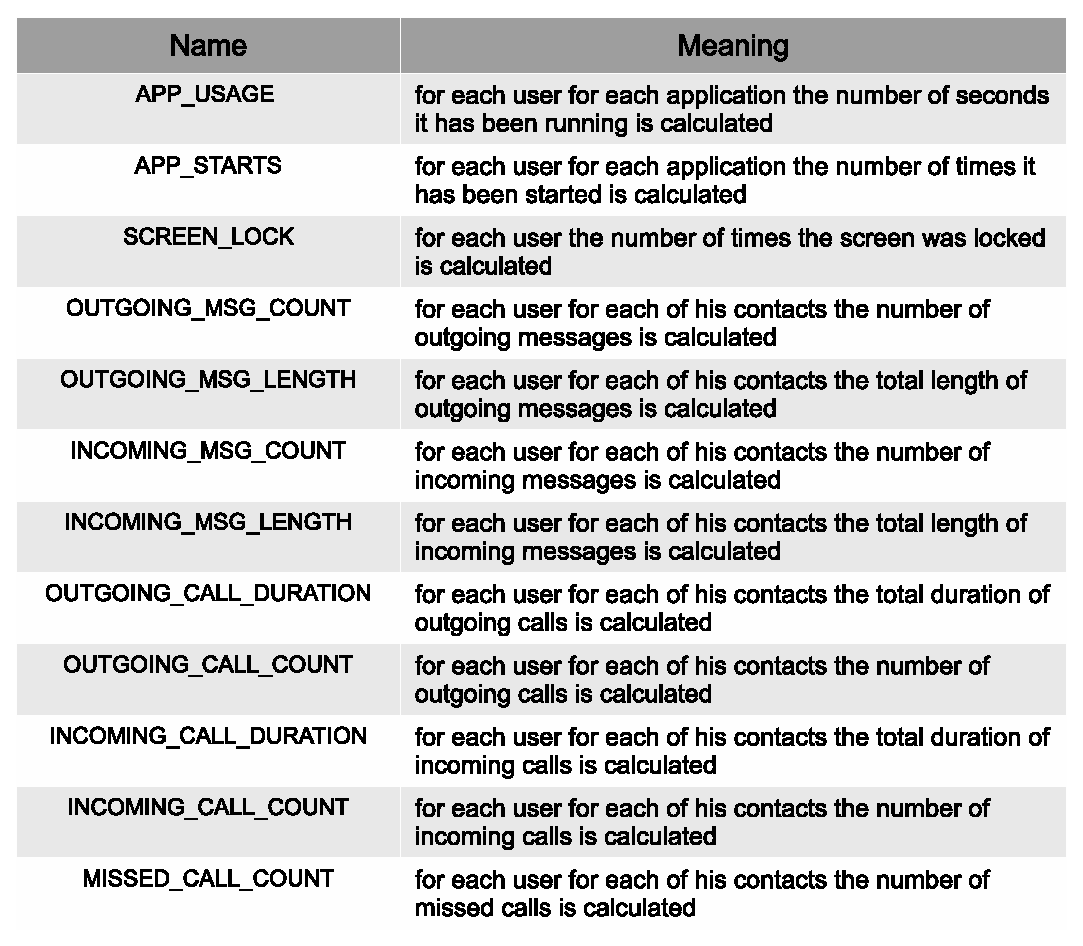
\includegraphics [width=1.0\textwidth]{images/user_based_aggregations}
  \caption{User-based aggregations}
  \label{fig:user_based_aggregations}
\end{figure}

The aggregations presented in the table are made for each user separately.
However, all these aggregations except SCREEN\_LOCK are also implemented as a sum and averadge for all users. 
Another group of aggregations is global summaries for different applications.
We calculate for each application the number of unique users, the number of sessions and total time spent. 

The implementation of aggregations in our case is based on Redis.
There is an interface \textit{EventAggregator} that actually allows to use any other data storages.
However, in our work we concentrate on Redis implementation of this interface.
It perfectly fits our needs for fast access and this storage is easy to use and does not need a lot of programming effort.


Anomaly Detection

People download various applications for their smartphones and do not pay much attention to the questions of security.
There is a risk that applications from unofficial stores contain the malicious software.
Moreover, the software from an official store can turn out to be infected.
The main problem is that usually users do not read what personal information the application requests an acces to.
And even if they read it, they do not have a choice to give the permissions or not.
Whithout giving the requred access rights, a user can not install this application on the smartphone.
   
The malicious software on smartphones behaves in different ways.
It can try to spread and infect all the contacts in a user's contact list.
For instance, a virus can send an sms, that contains its copy.
The virus can download and install another malicious software on the user's smartphone.
To apply some changes that the virus has performed in the system, it can restart the device.
Sometimes the malicious software can even make calls to specific numbers, so the user is charged for them.

\mnote{anomaly type}
As it was mentioned in Chapter , there are a lot of ways to detect anomaly in incoming data.
Let us first decide what kind of anomaly we are dealing with.
Ususally users do not have a strict pattern of interacting with their smartphones.
The sequence of performed actions changes from time to time.
One day a user can start with a phone call, another day by sending several messages.
This means that our anomaly is not \textit{collective}.
We consider a data instance independently from neighboring instances, therefore the anomaly type is not \textit{contextual}.
Thus we can conclude that we are dealing with the \textit{point} anomaly.

\mnote{anomaly detection approach}
Next step is to decide what approach to use for point anomaly detection.
The percentage of infected smartphones among the Menthal users is low.
It happens because the Android platform has good protection mechanisms and the official application stores are regularly tested for viruses.
Therefore we have a lot of \textit{normal} data and it is hard to get \textit{abnormal} examples (data from infected phones).
In this situation we can not use supervised learning, so we have chosen an unsupervised approach.

\mnote{One-class SVM}
There are several anomaly detection techniques that implement an unsupervised approach.
We decided to use one-class support vector machichenes (SVM) technique, because it perfectly fits our demands.
First, it needs only 'normal' data instances for learning.
Also it can work with high-dimension data, i.e. when a feature vector consists of more than two features (we need four in our case).
Moreover, there is an existing java library called libsvm [http://www.csie.ntu.edu.tw/~cjlin/libsvm/] that among other techniques implements one-class SVM.

Follow the assumed malicious software behavior, we try to detect the suspicious behavior of the smartphone.
For this purpose we analyze four events that are received from the clients: \textit{sms\_sent}, \textit{app\_install}, \textit{phone\_shutdown} and \textit{call\_outgoing}.
For simplicity we only count the number of these events.
However there is a possibility to make more thoroughtful research, using the values that these events contain.
For example, traffic data, namely the number of transferres bytes, can be used for analysis.
To have a basis for comparing the amount of events, we use a time window.
In other words, for each type of event we calculate the number of times it occures in a specified time interval (one hour by default).
Roughly speaking, we can take the number of times the event occures in a normal state, than calculate this number for an unknown state and make a conclusion whether it is normal or abnormal.

To use One-class SVM algorithm we need to create a training data set.
% TODO: write about training data

When the training set is ready we run \textit{svm\_train} method to create a model.
Then we use \textit{svm\_save\_model} method to safe the trained model, so it can be used later for anomaly detection.

\mnote{flow of events}
The Speed Layer has the following architecture to allow anomaly detection of incoming data.
Figure~\ref{fig:anomaly_detection_data_flow} illustrates the data flow.

\begin{figure}[h]
  \centering
  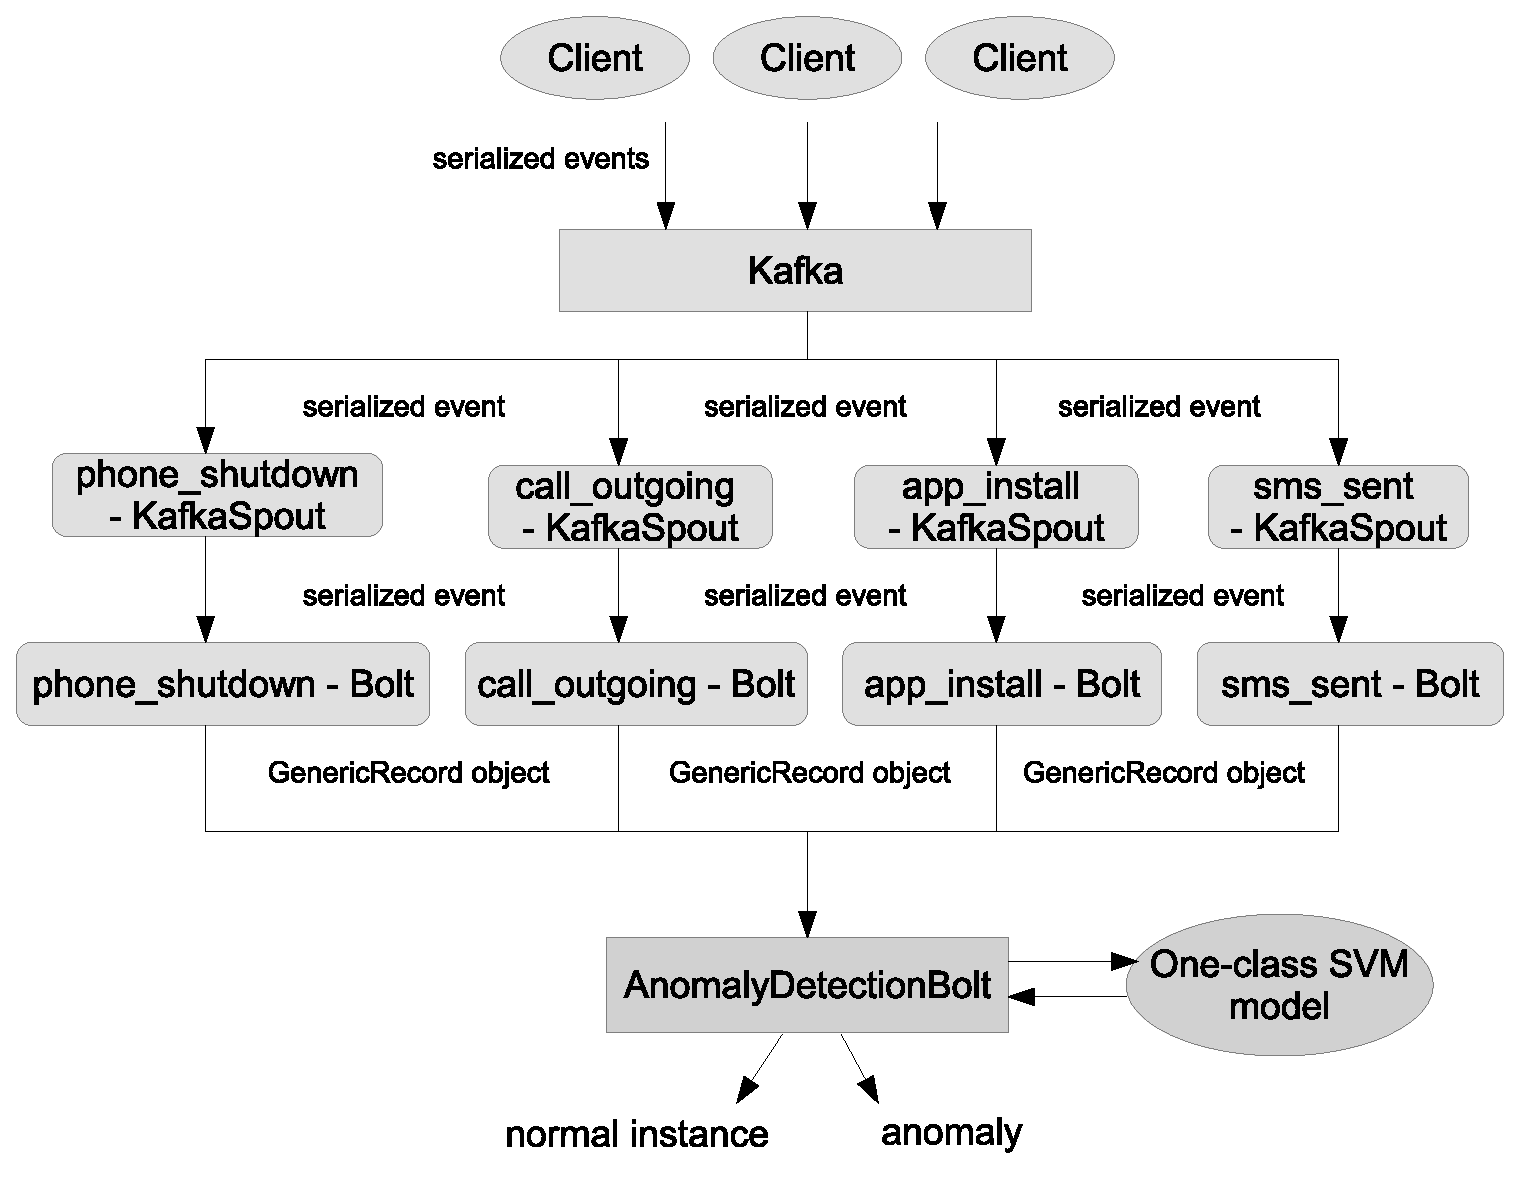
\includegraphics [width=1.0\textwidth]{images/anomaly_detection_data_flow}
  \caption{Anomaly detection: data flow}
  \label{fig:anomaly_detection_data_flow}
\end{figure}

For each Kafka topic a separate KafkaSpout receives messages.
One message contains the description of a particular event that happened on the client side (e.g. sms\_sent).
For each event type a separate bolt receives data from a corresponding KafkaSpout.
Then the bolt deserializes the received message, creating a \textit{GenericRecord} that represents the event.
For the events that are interesting for anomaly detection, there is an additional step.
Bolts, that receive data of type \textit{sms\_sent}, \textit{app\_install}, \textit{phone\_shutdown} and \textit{call\_outgoing}, emit the created GenericRecords to an \textit{AnomalyDetectionBolt}.

\mnote{Anomaly Detection bolt}
The main function of AnomalyDetectionBolt is to form data instances from incoming events.
As our version of Speed layer uses Redis as a data store, AnomalyDetectionBolt also uses it to accumulate events.
When a new event is received, AnomalyDetectionBolt extracts a type of event, a user id, and time when this event occured.
Using the user id, the bolt requests the value of \textit{lastCheckTime} that is stored in Redis.
The \textit{lastCheckTime} value is compared with the time, extracted from the received event.
If the time delta is bigger than a specified threshold, the new check for anomaly is performed.
The frequency of anomaly checks is regulated by an ANOMALY\_CHECK\_INTERVAL parameter.
This mechanism sets only one-side bound, so the check is performed not more than every half an hour by default.
However, if the bolt rare receives events from a particular user, the check for anomaly is run with the same low frequency. 

AnomalyDetectionBolt uses a sliding window to accumulate events.
The size of the window is regulated by a TTL parameter.
TTL specifies how long the event is stored in Redis.
Each time the new check for anomaly is performed, the bolt first of all deletes all outdated events from the store.
This guarantees that the data instance that participate in anomaly detection contains events that are collected over a specified period.
For example, the size of the sliding window is one hour by default.
If we want to perform an anomaly detection analysis, we take the mentioned earlier four types of events and count how many times each of them has occured during the last hour.
Using this numbers the bolt forms a data instance.  
Then it checks whether the instance is an anomaly or not using the trained one-class SVM model.

To get correct results it is essential to select the optimal parameters for One-class SVM.
Figure~\ref{fig:svm_parameters} represents the parameters, their meaning and values that are optimal for our case.
The process of parameters selection includes a technique called \textit{cross-validation}.
Here the data set is divided into two parts - training set and testing set.
This helps to avoid the problem of model overfitting.  

\begin{figure}[h]
  \centering
  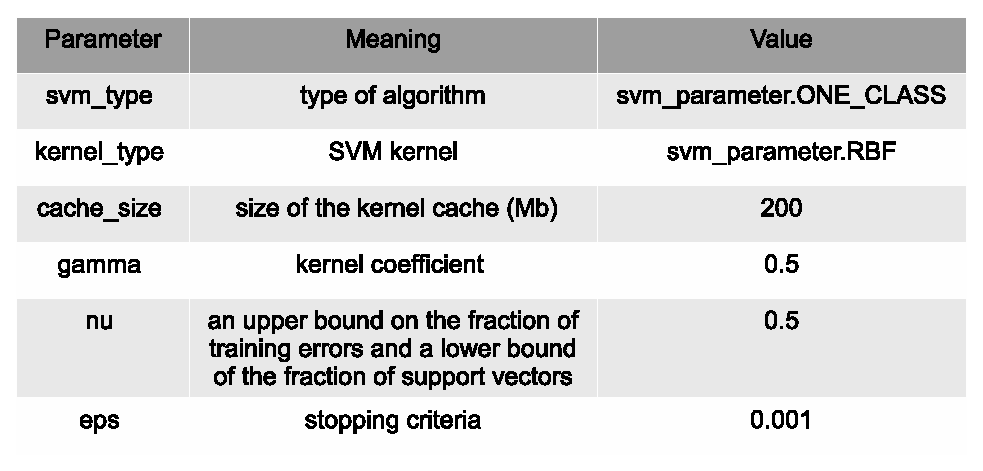
\includegraphics [width=0.9\textwidth]{images/svm_parameters}
  \caption{One-class SVM parameters}
  \label{fig:svm_parameters}
\end{figure}







 	

 
 

\input{content/10-Experiments}
\chapter{Summary [VI]}
\label{chap:summary}

The maintainance and processing of the large amounts of data has become a serious issue in the present time.
We have now the immense volume of data from many different sources.
And we can store it for a very low price.
However, it has brought us to the need to invent new methods and approaches of data storage, manipulation and processing.
We need to store it so, that it is robust and can be efficiently accessed.
We must be able to process it in a linearly scalable way.
As a result, the whole new field of computer science and information technology arised - namely Big Data.

In this thesis we have considered the new generic approach for the big data systems - the Lambda architecture.
We started with the description of the Menthal project, that encountered a problem to store and process large amounts of data.
Then we described the classical approaches to do that.
We showed examples of how Google and Facebook solve several big data issues.
Then we examined why and how those standard methods do not fulfill all the requirements of the generic big data system.
We investigated the Lambda architecture, that combines two approaches of data processing - batch and incremental.
We have designed and developed the Speed layer of the Lambda architecture, that completes the whole system in the Menthal project.
We conducted several experiments to measure and compare efficiency of two data processing frameworks - Spark and Storm.

The result of our work is the system, namely the Speed layer of the Lambda architecture, and also practical measurement of this implementation.
To make this system more robust, efficient and flexible additional investigation is required.
Research on different storage systems must be made.
More different setups of the cluster can be tested to achieve good performance.


%% Bibliographie
\backmatter
%\nocite{*}
\bibliography{bibliography/literature}

\appendix
\listoffigures
\listoftables
\lstlistoflistings

\end{document}
